% Options for packages loaded elsewhere
\PassOptionsToPackage{unicode}{hyperref}
\PassOptionsToPackage{hyphens}{url}
\PassOptionsToPackage{dvipsnames,svgnames*,x11names*}{xcolor}
%
\documentclass[
  11pt,
  letterpaper,
]{article}
\usepackage{lmodern}
\usepackage{setspace}
\usepackage{amssymb,amsmath}
\usepackage{ifxetex,ifluatex}
\ifnum 0\ifxetex 1\fi\ifluatex 1\fi=0 % if pdftex
  \usepackage[T1]{fontenc}
  \usepackage[utf8]{inputenc}
  \usepackage{textcomp} % provide euro and other symbols
\else % if luatex or xetex
  \usepackage{unicode-math}
  \defaultfontfeatures{Scale=MatchLowercase}
  \defaultfontfeatures[\rmfamily]{Ligatures=TeX,Scale=1}
\fi
% Use upquote if available, for straight quotes in verbatim environments
\IfFileExists{upquote.sty}{\usepackage{upquote}}{}
\IfFileExists{microtype.sty}{% use microtype if available
  \usepackage[]{microtype}
  \UseMicrotypeSet[protrusion]{basicmath} % disable protrusion for tt fonts
}{}
\makeatletter
\@ifundefined{KOMAClassName}{% if non-KOMA class
  \IfFileExists{parskip.sty}{%
    \usepackage{parskip}
  }{% else
    \setlength{\parindent}{0pt}
    \setlength{\parskip}{6pt plus 2pt minus 1pt}}
}{% if KOMA class
  \KOMAoptions{parskip=half}}
\makeatother
\usepackage{xcolor}
\IfFileExists{xurl.sty}{\usepackage{xurl}}{} % add URL line breaks if available
\IfFileExists{bookmark.sty}{\usepackage{bookmark}}{\usepackage{hyperref}}
\hypersetup{
  pdftitle={Case-Enabled Reasoning Engine with Bayesian Representations for Unified Modeling (CEREBRUM)},
  pdfauthor={Daniel Ari Friedman},
  colorlinks=true,
  linkcolor=black,
  filecolor=Maroon,
  citecolor=Blue,
  urlcolor=black,
  pdfcreator={LaTeX via pandoc}}
\urlstyle{same} % disable monospaced font for URLs
\usepackage[margin=1in]{geometry}
\usepackage{color}
\usepackage{fancyvrb}
\newcommand{\VerbBar}{|}
\newcommand{\VERB}{\Verb[commandchars=\\\{\}]}
\DefineVerbatimEnvironment{Highlighting}{Verbatim}{commandchars=\\\{\}}
% Add ',fontsize=\small' for more characters per line
\newenvironment{Shaded}{}{}
\newcommand{\AlertTok}[1]{\textcolor[rgb]{1.00,0.00,0.00}{\textbf{#1}}}
\newcommand{\AnnotationTok}[1]{\textcolor[rgb]{0.38,0.63,0.69}{\textbf{\textit{#1}}}}
\newcommand{\AttributeTok}[1]{\textcolor[rgb]{0.49,0.56,0.16}{#1}}
\newcommand{\BaseNTok}[1]{\textcolor[rgb]{0.25,0.63,0.44}{#1}}
\newcommand{\BuiltInTok}[1]{#1}
\newcommand{\CharTok}[1]{\textcolor[rgb]{0.25,0.44,0.63}{#1}}
\newcommand{\CommentTok}[1]{\textcolor[rgb]{0.38,0.63,0.69}{\textit{#1}}}
\newcommand{\CommentVarTok}[1]{\textcolor[rgb]{0.38,0.63,0.69}{\textbf{\textit{#1}}}}
\newcommand{\ConstantTok}[1]{\textcolor[rgb]{0.53,0.00,0.00}{#1}}
\newcommand{\ControlFlowTok}[1]{\textcolor[rgb]{0.00,0.44,0.13}{\textbf{#1}}}
\newcommand{\DataTypeTok}[1]{\textcolor[rgb]{0.56,0.13,0.00}{#1}}
\newcommand{\DecValTok}[1]{\textcolor[rgb]{0.25,0.63,0.44}{#1}}
\newcommand{\DocumentationTok}[1]{\textcolor[rgb]{0.73,0.13,0.13}{\textit{#1}}}
\newcommand{\ErrorTok}[1]{\textcolor[rgb]{1.00,0.00,0.00}{\textbf{#1}}}
\newcommand{\ExtensionTok}[1]{#1}
\newcommand{\FloatTok}[1]{\textcolor[rgb]{0.25,0.63,0.44}{#1}}
\newcommand{\FunctionTok}[1]{\textcolor[rgb]{0.02,0.16,0.49}{#1}}
\newcommand{\ImportTok}[1]{#1}
\newcommand{\InformationTok}[1]{\textcolor[rgb]{0.38,0.63,0.69}{\textbf{\textit{#1}}}}
\newcommand{\KeywordTok}[1]{\textcolor[rgb]{0.00,0.44,0.13}{\textbf{#1}}}
\newcommand{\NormalTok}[1]{#1}
\newcommand{\OperatorTok}[1]{\textcolor[rgb]{0.40,0.40,0.40}{#1}}
\newcommand{\OtherTok}[1]{\textcolor[rgb]{0.00,0.44,0.13}{#1}}
\newcommand{\PreprocessorTok}[1]{\textcolor[rgb]{0.74,0.48,0.00}{#1}}
\newcommand{\RegionMarkerTok}[1]{#1}
\newcommand{\SpecialCharTok}[1]{\textcolor[rgb]{0.25,0.44,0.63}{#1}}
\newcommand{\SpecialStringTok}[1]{\textcolor[rgb]{0.73,0.40,0.53}{#1}}
\newcommand{\StringTok}[1]{\textcolor[rgb]{0.25,0.44,0.63}{#1}}
\newcommand{\VariableTok}[1]{\textcolor[rgb]{0.10,0.09,0.49}{#1}}
\newcommand{\VerbatimStringTok}[1]{\textcolor[rgb]{0.25,0.44,0.63}{#1}}
\newcommand{\WarningTok}[1]{\textcolor[rgb]{0.38,0.63,0.69}{\textbf{\textit{#1}}}}
\usepackage{longtable,booktabs}
% Correct order of tables after \paragraph or \subparagraph
\usepackage{etoolbox}
\makeatletter
\patchcmd\longtable{\par}{\if@noskipsec\mbox{}\fi\par}{}{}
\makeatother
% Allow footnotes in longtable head/foot
\IfFileExists{footnotehyper.sty}{\usepackage{footnotehyper}}{\usepackage{footnote}}
\makesavenoteenv{longtable}
\usepackage{graphicx}
\makeatletter
\def\maxwidth{\ifdim\Gin@nat@width>\linewidth\linewidth\else\Gin@nat@width\fi}
\def\maxheight{\ifdim\Gin@nat@height>\textheight\textheight\else\Gin@nat@height\fi}
\makeatother
% Scale images if necessary, so that they will not overflow the page
% margins by default, and it is still possible to overwrite the defaults
% using explicit options in \includegraphics[width, height, ...]{}
\setkeys{Gin}{width=\maxwidth,height=\maxheight,keepaspectratio}
% Set default figure placement to htbp
\makeatletter
\def\fps@figure{htbp}
\makeatother
\setlength{\emergencystretch}{3em} % prevent overfull lines
\providecommand{\tightlist}{%
  \setlength{\itemsep}{0pt}\setlength{\parskip}{0pt}}
\setcounter{secnumdepth}{-\maxdimen} % remove section numbering
\usepackage{etoolbox}\pretocmd{\section}{\clearpage}{}{}

\title{Case-Enabled Reasoning Engine with Bayesian Representations for
Unified Modeling (CEREBRUM)}
\author{Daniel Ari Friedman}
\date{Version 1.0 (2025-04-07)}

\begin{document}
\maketitle
\begin{abstract}
This paper introduces Case-Enabled Reasoning Engine with Bayesian
Representations for Unified Modeling (CEREBRUM). CEREBRUM is a synthetic
intelligence framework that integrates linguistic case systems with
cognitive scientific principles to describe, design, and deploy
generative models in an expressive fashion. By treating models as
case-bearing entities that can play multiple contextual roles (e.g.~like
declinable nouns), CEREBRUM establishes a formal linguistic-type
calculus for cognitive model use, relationships, and transformations.
The CEREBRUM framework uses structures from category theory and modeling
techniques related to the Free Energy Principle, in describing and
utilizing models across contexts. CEREBRUM addresses the growing
complexity in computational and cognitive modeling systems
(e.g.~generative, decentralized, agentic intelligences), by providing
structured representations of model ecosystems that align with lexical
ergonomics, scientific principles, and operational processes.
\end{abstract}

{
\hypersetup{linkcolor=}
\setcounter{tocdepth}{2}
\tableofcontents
}
\setstretch{1.15}
\hypertarget{overview}{%
\section{Overview}\label{overview}}

CEREBRUM implements a comprehensive approach to cognitive systems
modeling by applying linguistic case systems to model management. This
framework treats cognitive models as entities that can exist in
different ``cases'', as in a morphologically rich language, based on
their functional role within an intelligence production workflow. This
enables more structured representation of model relationships and
transformations. The code to generate this paper, and further open
source development from this 1.0 milestone release, is available at
https://github.com/ActiveInferenceInstitute/CEREBRUM . \# Background
\#\# Cognitive Systems Modeling Cognitive systems modeling approaches
cognition as a complex adaptive system, where cognitive processes emerge
from the dynamic interaction of multiple components across different
scales. This perspective draws from ecological psychology's emphasis on
organism-environment coupling, where cognitive processes are
fundamentally situated in and shaped by their environmental context. The
4E cognition framework (embodied, embedded, enacted, and extended)
provides a theoretical foundation for understanding how cognitive
systems extend beyond individual agents to include environmental
structures and social interactions. In this view, cognitive models are
not merely internal representations but active participants in a broader
cognitive ecosystem, where they adapt and evolve through interaction
with other models and environmental constraints. This systems-level
perspective is particularly relevant for intelligence production, where
multiple analytical models must coordinate their activities while
maintaining sensitivity to changing operational contexts and
requirements. The complex adaptive systems approach emphasizes
self-organization, emergence, and adaptation, viewing cognitive
processes as distributed across multiple interacting components that
collectively produce intelligent behavior through their coordinated
activity (including language use). \#\# Active Inference Active
Inference is a first-principles account of perception, learning, and
decision-making based on the Free Energy Principle. In this framework,
cognitive systems minimize variational free energy bounded surprise,
reflecting the difference between an organism's internal model and its
environment through perception (updating internal models) and action
(changing action and ultimately sensory inputs). The Active Inference
framework formalizes uncertainty in terms of entropy and precision
weighting, enabling dynamic adaptive processes. While many model
architectures are possible, hierarchical message passing is a common
implementation that implements predictions as top-down flows and
prediction errors as bottom-up flows, creating a bidirectional inference
system that iteratively minimizes surprise across model levels. Active
Inference treats all cognitive operations as Bayesian model update,
providing a unifying mathematical formalism for predictive cognition.
\#\# Linguistic Case Systems Linguistic case systems represent
grammatical relationships between words through morphological marking.
Case systems operate as morphosyntactic interfaces between semantics and
syntax, encoding contextualized relationship types rather than just
sequential ordering. This inherent relationality makes case systems
powerful abstractions for modeling complex dependencies and
transformations between conceptual entities. Cases under consideration
here include nominative (subject), accusative (object), dative
(recipient), genitive (possessor), instrumental (tool), locative
(location), and ablative (origin), all serving different functional
roles within sentence structures. Languages implement these differently:
nominative-accusative systems distinguish subjects from objects, while
ergative-absolutive systems group intransitive subjects with direct
objects. While English has largely lost its morphological case system,
the underlying case relationships still exist and are expressed through
word order and prepositions. For example, in ``The cat chased the
mouse,'' the nominative case is marked by position (subject before verb)
rather than morphology, while in ``I gave him the book,'' the dative
case is marked by the preposition ``to'' (implied) and word order. This
demonstrates that (the semantics/semiosis/pragmatics of) case
relationships are fundamental to language structure, even when not
overtly marked morphologically (e.g.~expressed in writing or spoken
language). \#\# Intelligence Case Management Systems Intelligence case
management systems organize investigative workflows and analytical
processes in operational contexts. These systems structure information
collection, analysis, evaluation, and dissemination while tracking
provenance and relationships between intelligence products. Modern
implementations increasingly must manage complex model ecosystems where
analytical tools, data sources, and products interact within
organizational workflows. However, current frameworks lack formal
mathematical foundations for representing model relationships, leading
to ad hoc integration approaches that become unwieldy at scale. As
artificial intelligence components proliferate in these systems, a more
rigorous basis for model interaction becomes essential for maintaining
operational coherence and analytical integrity. \#\# Towards Languages
for Generative Modeling The Active Inference community has extensively
explored numerous adjectival modifications of the base framework,
including Deep, Affective, Branching-Time, Quantum, Mortal, Structured
Inference, among others. Each adjectival-prefixed variant emphasizes
specific architectural aspects or extensions of the core formalism.
Building on this, CEREBRUM focuses on a wider range of linguistic
formalism (e.g.~in this paper, declensional semantics) rather than
adjectival modifications. In this first CEREBRUM paper, there is an
emphasis on the declensional aspects of generative models as noun-like
entities, separate from adjectival qualification. This approach aligns
with category theoretic approaches to linguistics, where morphisms
between objects formalize grammatical relationships and transformations.
By applying formal case grammar to generative models, CEREBRUM extends
and transposes structured modeling approaches to ecosystems of shared
intelligence, while preserving the underlying (partitioned, flexible,
variational, composable, interfacial, inter-active, empirical,
applicable, communicable) semantics. \#\# Conceptual Foundations: The
Intersection of Four Domains CEREBRUM integrates four key domains to
create a unified framework for model management (Figure 1): 1.
\textbf{Cognitive Systems Modeling} offers the entities that take on
case relationships 2. \textbf{Active Inference} supplies the predictive
processing mechanics that drive case transformations 3.
\textbf{Linguistic Case Systems} provide the grammatical metaphor for
how models relate to each other 4. \textbf{Intelligence Production}
furnishes the practical application context and workflows \#\# Methods
and Materials \#\# Formal Framework Development The CEREBRUM framework
was developed as a part of a broader synthetic intelligence framework,
combining linguistic theory, cognitive science, category theory, and
operations research. Key methodological approaches included: 1.
\textbf{Linguistic Formalization}: Adapting morphosyntactic case theory
into computational representations through abstract algebraic
structures. 2. \textbf{Category-Theoretic Mapping}: Implementing
category theory to formalize morphisms between case states as functorial
transformations. 3. \textbf{Algorithmic Implementation}: Developing
algorithmic specifications for case transformations compliant with the
Free Energy Principle. 4. \textbf{Variational Methods}: Applying
variational free energy calculations to optimize model inference as well
as structural transformations. \#\# Mathematical Foundation The
mathematical foundation of CEREBRUM builds on formalizations of case
transformations using category theory and variational inference. Case
transformations are modeled as morphisms in a category where objects are
models with specific case assignments. The framework employs metrics
including Kullback-Leibler divergence, Fisher information, and Lyapunov
functions to quantify transformation efficacy and system stability. This
approach provides both theoretical guarantees of compositional
consistency and practical optimization methods for computational
implementation. \#\# Core Concept: Cognitive Models as Case-Bearing
Entities Just as nouns in morphologically rich languages take different
forms based on their grammatical function, cognitive models in CEREBRUM
can exist in different ``states'' or ``cases'' depending on how they
relate to other models or processes within the system. Figure 2
illustrates this linguistic parallel. !{[}F igure 2: illustrates this
linguistic parallel. !{[}F igure 2: illustrates this linguistic
parallel. !{[}F igure 2: illustrates this linguistic parallel. !{[}F
igure 2: illustrates this linguistic parallel. !{[}F igure 2:
illustrates this linguistic parallel. igure 2: illustrates this
linguistic parallel. \#\# Case Functions in Cognitive Modeling Each case
defines a sp ecific relationship type between models or between models
and data (Table 1). The basic framework is depicted in Figure 3.
\textbf{Table 1: Case Functions in Cognitive Model Systems} \textbar{}
Abbr \textbar{} Case \textbar{} Function in CEREBRUM \textbar{} Example
Usage \textbar{}
\textbar------\textbar------\textbar----------------------\textbar---------------\textbar{}
\textbar{} \textbf{{[}NOM{]}} \textbar{} \textbf{Nominative} \textbar{}
Model as active agent; acts as the primary producer of predictions and
exerts causal influence on other models \textbar{} Model X {[}NOM{]}
generates predictions about data distributions; controls downstream
processing \textbar{} \textbar{} \textbf{{[}ACC{]}} \textbar{}
\textbf{Accusative} \textbar{} Model as object of process; receives
transformations and updates from other models or processes \textbar{}
Process applies to Model X {[}ACC{]}; optimization procedures refine
Model X's parameters \textbar{} \textbar{} \textbf{{[}GEN{]}} \textbar{}
\textbf{Genitive} \textbar{} Model as source/possessor; functions as the
origin of outputs, products, and derived models \textbar{} Output of
Model X {[}GEN{]}; intelligence products derived from Model X's
inferences \textbar{} \textbar{} \textbf{{[}DAT{]}} \textbar{}
\textbf{Dative} \textbar{} Model as recipient; specifically configured
to receive and process incoming data flows \textbar{} Data fed into
Model X {[}DAT{]}; Model X receives information from external sources
\textbar{} \textbar{} \textbf{{[}INS{]}} \textbar{}
\textbf{Instrumental} \textbar{} Model as method/tool; serves as the
means by which analytical operations are performed \textbar{} Analysis
performed via Model X {[}INS{]}; Model X implements analytical
procedures \textbar{} \textbar{} \textbf{{[}LOC{]}} \textbar{}
\textbf{Locative} \textbar{} Model as context; provides environmental
constraints and situational parameters \textbar{} Parameters within
Model X {[}LOC{]}; environmental contingencies modeled by X \textbar{}
\textbar{} \textbf{{[}ABL{]}} \textbar{} \textbf{Ablative} \textbar{}
Model as origin/cause; represents historical conditions or causal
precursors \textbar{} Insights derived from Model X {[}ABL{]}; causal
attributions traced to Model X \textbar{} \textbar{} \textbf{{[}VOC{]}}
\textbar{} \textbf{Vocative} \textbar{} Model as addressable entity;
functions as a directly callable interface with name-based activation
\textbar{} ``Hey Model X'' {[}VOC{]}; direct invocation of Model X for
task initialization; documentation reference point \textbar{} Within
intelligence production systems, these case relationships serve critical
functional roles: nominative models act as primary analytical engines
driving the intelligence case; accusative models become targets of
quality assessment and improvement; multimodal genitive models generate
documentation and reports; dative models receive and process collected
intelligence data; instrumental models provide the methodological
framework for investigations; locative models establish situational
boundaries; ablative models represent the historical origins of
analytical conclusions; and vocative models serve as directly
addressable interfaces for command initiation and documentation
reference. Together, these case relationships create a comprehensive
framework for structu red intelligence workflows. Figure 4 illustrates
how this core framework integrates with intelligence case management.
\#\# A Preliminary Example of a Case-Bearing Model: Homeostatic
Thermostat Consider a cognitive model of a homeostatic thermostat that
perceives room temperature with a thermometer, and regulates temperature
through connected heating and cooling systems. In nominative case
{[}NOM{]}, the thermostat model actively generates temperature
predictions and dispatches control signals, functioning as the primary
agent in the temperature regulation process. When placed in accusative
case {[}ACC{]}, this same model becomes the object of optimization
processes, with its parameters being updated based on prediction errors
between expected and actual temperature readings. In dative case
{[}DAT{]}, the thermostat model receives environmental temperature data
streams and occupant comfort preferences as inputs. The genitive case
{[}GEN{]} transforms the model into a generator of temperature
regulation reports and system performance analytics (``genitive AI'').
When in instrumental case {[}INS{]}, the thermostat serves as a
computational tool implementing control algorithms for other systems
requiring temperature management. The locative case {[}LOC{]}
reconfigures the model to represent the contextual environment in which
temperature regulation occurs, modeling building thermal properties, or
discussing something within the model as a location. Finally, in
ablative case {[}ABL{]}, the thermostat functions as the origin of
historical temperature data and control decisions, providing causal
explanations for current thermal conditions. This single cognitive model
thus assumes dramatically different functional roles while maintaining
its core identity as a thermostat. \#\# Declinability of Active
Inference Generative Models At the core of CEREBRUM lies the concept of
\textbf{declinability} - the capacity for generative models to assume
different morphological and functional roles through case
transformations, mirroring the declension patterns of nouns in
morphologically rich languages. Unlike traditional approaches where
models maintain fixed roles, or variable roles defined by analytical
pipelines, CEREBRUM treats cognitive models as flexible entities capable
of morphological adaptation to different operational contexts. \#\#
Morphological Transformation of Generative Models When an active
inference generative model undergoes case transformation, it experiences
orchestrated systematic changes summarized in Table 2: 1.
\textbf{Functional Interfaces}: Input/output specifications change to
match the case role requirements 2. \textbf{Parameter Access Patterns}:
Which parameters are exposed or constrained changes based on case 3.
\textbf{Prior Distributions}: Different cases employ different prior
constraints on parameter values 4. \textbf{Update Dynamics}: The ways in
which the model updates its internal states vary by case role 5.
\textbf{Computational Resources}: Different cases receive different
precision-weighted computational allocations \textbf{Table 2:
Transformational Properties of Active Inference Generative Models Under
Case Declensions} \textbar{} Case \textbar{} Parametric Changes
\textbar{} Interface Transformations \textbar{} Precision Weighting
\textbar{}
\textbar------\textbar-------------------\textbar--------------------------\textbar-------------------\textbar{}
\textbar{} \textbf{{[}NOM{]}} \textbar{} Fully accessible parameters;
all degrees of freedom available for prediction generation; strongest
prior constraints on likelihood mapping \textbar{} Outputs predictions;
exposes forward inference pathways; prediction interfaces activated
\textbar{} Highest precision on likelihood; maximizes precision of
generative mapping from internal states to observations \textbar{}
\textbar{} \textbf{{[}ACC{]}} \textbar{} Restricted parameter access;
plasticity gates opened; learning rate parameters prioritized \textbar{}
Receives transformations; update interfaces exposed; gradient reception
pathways active \textbar{} Highest precision on parameters; maximizes
precision of parameter updates based on prediction errors \textbar{}
\textbar{} \textbf{{[}DAT{]}} \textbar{} Input-focused parameterization;
sensory mapping parameters prioritized; perceptual categorization
parameters activated \textbar{} Receives data flows; input processing
interfaces exposed; sensory reception channels active \textbar{} Highest
precision on inputs; maximizes precision of incoming data relative to
internal expectations \textbar{} \textbar{} \textbf{{[}GEN{]}}
\textbar{} ``Genitive AI''; Output-focused parameterization; production
parameters activated; generative pathway emphasis \textbar{} Generates
products; output interfaces prioritized; production pathways activated
\textbar{} Highest precision on outputs; maximizes precision of
generated products relative to internal models \textbar{} \textbar{}
\textbf{{[}INS{]}} \textbar{} Method-oriented parameters exposed;
algorithmic parameters accessible; procedural knowledge emphasized
\textbar{} Implements processes; computational interfaces active;
procedural execution pathways open \textbar{} Highest precision on
operations; maximizes precision of procedural execution relative to
methodological expectations \textbar{} \textbar{} \textbf{{[}LOC{]}}
\textbar{} Context parameters emphasized; environmental modeling
parameters prioritized; situational knowledge emphasized \textbar{}
Provides environmental constraints; contextual interfaces active;
environmental modeling pathways prioritized \textbar{} Highest precision
on contexts; maximizes precision of contextual representation relative
to environmental dynamics \textbar{} \textbar{} \textbf{{[}ABL{]}}
\textbar{} Origin states emphasized; historical parameters accessible;
causal attribution pathways strengthened \textbar{} Source of
information; historical data interfaces active; causal explanation
pathways open \textbar{} Highest precision on historical data; maximizes
precision of causal attributions and historical reconstructions
\textbar{} \textbar{} \textbf{{[}VOC{]}} \textbar{} Identity parameters
prioritized; naming and identification parameters activated; interface
exposure emphasized \textbar{} Maintains addressable interfaces; name
recognition pathways activated; command reception channels open
\textbar{} Highest precision on identification cues; maximizes precision
of name recognition relative to calling patterns \textbar{} \#\# Active
Inference Model Declension Example Consider a perception-oriented
generative model M with parameters theta, internal states s, and
observational distribution p(o\textbar s,theta). When declined across
cases, this single model transforms as follows: - \textbf{M{[}NOM{]}}:
Actively generates predictions by sampling from p(o\textbar s,theta),
with all parameters fully accessible - \textbf{M{[}ACC{]}}: Becomes the
target of updates, with parameter gradients calculated from prediction
errors - \textbf{M{[}DAT{]}}: Configured to receive data flows, with
specific input interfaces activated - \textbf{M{[}GEN{]}}: Optimized to
generate outputs, with output interfaces prioritized -
\textbf{M{[}INS{]}}: Functions as a computational method, exposing
algorithmic interfaces - \textbf{M{[}LOC{]}}: Provides contextual
constraints for other models, with environmental parameters exposed -
\textbf{M{[}ABL{]}}: Serves as an information source, with historical
data accessible - \textbf{M{[}VOC{]}}: Functions as an addressable
entity responding to direct invocation, with naming parameters activated
The Vocative case {[}VOC{]} represents a unique functional role where
models serve as directly addressable entities within a model ecosystem.
Unlike other cases that focus on data processing or transformational
aspects, the vocative case specifically optimizes a model for name-based
recognition and command reception. This has particular relevance in
synthetic intelligence environments where models must be selectively
activated or ``woken up'' through explicit address, similar to how
humans are called by name to gain their attention. The vocative case
maintains specialized interfaces for handling direct commands,
documentation references, and initialization requests. In practical
applications, models in vocative case might serve as conversational
agents awaiting activation, documentation reference points within
technical specifications, or system components that remain dormant until
explicitly addressed. This pattern mimics the linguistic vocative case
where a noun is used in direct address, as in ``Hey Siri'' or ``OK
Google'' activation phrases for digital assistants, creating a natural
bridging pattern between human language interaction and model
orchestration. This systematic pattern of transformations constitutes a
complete ``declension paradigm'' for cognitive models, using
precision-modulation to fulfill diverse functional roles while
maintaining their core identity. \#\# Model Workflows as Case Transfor m
a tions Case transformations rep resent operations that change the fun
ctional role o f a model in the system, reflecting active inferenc e
principles of predictio n and error minimization. Figure 5 provides a
sequence diagram of a typical transformation cycle, and Figur es/) .png)
es/) ) es/) () es/) f a typical transformation cycle, and Figur es/) e 6
shows the intelligence production workflow where these transformations
occur. mation cycle, and Figure 6 s hows the intelligence productio n
workflow where these transformations occur. es/) ions occur. \#\#
Category-Theoretic Formalization CEREBRUM employs category theory to
formalize case relationships between cognitive models, creating a
rigorous mathematical foundation, illustrated in Figure 7 and Figure 8.
\#\# Computational Linguistics, Structural Alignment, and Model
Relationships CEREBRUM supports different alignment systems for model
relationships, mirroring ling uistic morphosyntactic struc tures (Figure
9). These alignment patterns determine how models interact and transform
based on their functional ro les. Figure 9 illustrates the core
alignment patterns derived from linguistic theory, showing how models
can be organized based on their case relationships. This includes
nominative-accusative alignment (where models are distinguished by their
role as agents or patients), ergative-absolutive alignment (where models
are grouped by their relationship to actions), and tripartite alignment
(where each case is marked distinctly). nd tripartite alignment (where
each case is marked distinctly). \_12.png) igure\_9.png) Figure 10
demonstrates the practical imple \_12.png) mentation of these alignment
patterns in model ecosystems, showing ) \_12.png) entation view
complements the the \_12.png) \_12.png) \_12.png) oretical alignment
patterns shown in Figure 9 by demonstrating their practical application
in cognitive model management. how different alignment systems affect
model interactions and transformations. The diagram illustrates the
computational implications of each alignment pattern, including resource
allocation, message passing, and transformation efficiency. This
implementation view complements the theoretical alignment patterns shown
in Figure 9 by demonstrating their practical application in cognitive
model management. \#\# Implementation in Intelligence Production As
mentioned, CEREBRUM integrates with intelligence case management through
structured workflows (see Figures 4 and 6). Figure 11 and Figure 12
provide alternative state-based visualizations of these workflows. ing
rules. ) ing rules. 4.png) g) The intelligence production workflow ing
rules. begins with raw data collection, where models in instrumental
case {[}INS{]} ser ve as data collection to ols, implementing specific
methods for information gathering. As data moves through preprocessing,
models transition to nominative case {[}NOM{]}, taking on active
processing roles to clean, normalize, and prepare the data for analysis.
During analysis, models assume locative case {[}LOC{]}, providing
contextual understanding and environmental parameters that shape the
analytical process. Integration represents a critical transition point
where models in genitive case {[}GEN{]} generate intelligence products
by synthesizi ing rules. n ing rules. ing rules. g information from
multiple sources. These products then undergo evaluati on by models in
accusative case {[}ACC{]}, which assess quality and identify areas for
improvement. The refinement phase employs models in dative case
{[}DAT{]} to process feedback and implement necessary changes, while
deployment returns models to nominative case {[}NOM{]} for active
implementation of refined solutions. This cyclical process demonstrates
how case transformations enable models to maintain their core identity
while adapting to different functional requirements throughout the
intelligence production lifecycle. Each case assignment optimizes
specific aspects of model behavior, from data collection and processing
to product generation and quality assessment, creating a flexible yet
structured approach to intelligence production. \#\# Active Inference
Integration CEREBRUM aligns with active inference frameworks by treating
case transformations as predictive processes within a free energy
minimization framework, as illustrated in Figure 13. Figure 14 details
the associated message passing rules. \#\# Formal Case Calculus The
relationships between case-bearing models follow a formal calculus
derived from grammatical case systems, presented in Figure 15. \#\#
Cross-Domain Integration Benefits The CEREBRUM framework delivers
several advantages through its integration of the four foundational
domains: \textbf{Table 4: Cross-Domain Integration Benefits in CEREBRUM
Framework} \textbar{} Domain \textbar{} Contribution \textbar{} Benefit
to CEREBRUM \textbar{} Theoretical Significance \textbar{}
\textbar--------\textbar--------------\textbar---------------------\textbar--------------------------\textbar{}
\textbar{} \textbf{Linguistic Case Systems} \textbar{} Systematic
relationship framework; grammatical role templates; morphosyntactic
structures \textbar{} Structured representation of model interactions;
formalized functional transitions; systematic role assignment \textbar{}
Provides formal semantics for model relationships; enables compositional
theory of model interactions; grounds functions in linguistic universals
\textbar{} \textbar{} \textbf{Cognitive Systems Modeling} \textbar{}
Entity representation and processing; model formalization;
information-processing structures \textbar{} Flexible model
instantiation across functional roles; adaptive model morphology;
unified modeling paradigm \textbar{} Advances theory of cognitive model
composition; formalizes functional transitions in cognitive systems;
bridges symbolic and statistical approaches \textbar{} \textbar{}
\textbf{Active Inference} \textbar{} Predictive transformation
mechanics; free energy principles; precision-weighted learning
\textbar{} Self-optimizing workflows with error minimization; principled
uncertainty handling; bidirectional message passing \textbar{} Extends
active inference to model ecosystems; provides mathematical foundation
for case transformations; unifies perception and model management
\textbar{} \textbar{} \textbf{Intelligence Production} \textbar{}
Practical operational context; analytical workflows; intelligence cycle
formalisms \textbar{} Real-world application in case management systems;
operational coherence; analytical integrity \textbar{} Bridges
theoretical and applied intelligence; enhances intelligence workflow
coherence; improves analytical product quality \textbar{} \#\# Related
Work CEREBRUM builds upon several research traditions while offering a
novel synthesis. In this first paper, there are no specific works linked
or cited. Later work will provide more detail in reference and
derivation. The work stands transparently on the shoulders of nestmates
and so is presented initially as a speculative design checkpoint in the
development of certain cognitive modeling practices. Related approaches
include: \#\# Cognitive Architectures CEREBRUM offers a novel approach
to intelligent system design, drawing inspiration from linguistic
declension to create flexible model architectures with dynamic role
assignment. Unlike traditional architectures with fixed component
functions, CEREBRUM enables cognitive models to adapt their functional
roles through case-based transformations, enhancing both flexibility and
specialization simultaneously. This contrasts with existing approaches
that often force a trade-off between these qualities. By applying
morphological transformations to generative models, CEREBRUM creates
polymorphic components that maintain their core identity while adapting
interfaces, parameters, and processing dynamics to context-specific
requirements. This architecture provides a principled foundation for
coordinating complex model ecosystems in intelligence production and
other cognitive computing applications. \#\# Category-Theoretic
Cognition The mathematical formalization of CEREBRUM through category
theory creates a foundation for compositional reasoning about cognitive
systems. By representing case transformations as functors between model
categories, the framework enables formal verification of transformation
properties, including preservation of model identity across functional
transitions. These category-theoretic foundations support reasoning
about model composition, transformation sequencing, and structural
relationships within model ecosystems. The richness of category theory's
compositional approach aligns with the inherently compositional nature
of cognitive processes, providing both theoretical insights and
practical guidelines for implementing complex cognitive architectures.
\#\# Active Inference Applications CEREBRUM extends the active inference
framework beyond individual cognitive processes to model ecosystems,
treating case transformations as precision-weighted processes that
minimize free energy across system boundaries. This approach enables
principled coordination of active inference models by explicitly
representing their functional relationships through case assignments. By
formalizing the interfaces between models using precision-weighting
mechanisms inspired by active inference, CEREBRUM creates intelligent
workflows where models cooperate to minimize system-wide free energy
while adapting their specific roles to changing requirements. This
extension of active inference principles to model orchestration bridges
the gap between theoretical neuroscience and practical application in
intelligence production. \#\# Linguistic Computing CEREBRUM represents a
novel linguistic approach to computing, applying declensional semantics
to model management. This perspective treats cognitive models as
entities that assume different morphological forms based on their
functional roles, mirroring how nouns in morphologically rich languages
change form depending on their grammatical function. By implementing
computable declension paradigms for models, CEREBRUM enables more
expressive and flexible representations of model relationships than
traditional object-oriented or functional paradigms alone. This
linguistically-inspired approach to model management provides both
conceptual clarity for human programmers and formal rigor for
computational implementations, creating a bridge between natural and
artificial intelligence systems. (See Supplement 2: Novel Linguistic
Cases for a discussion of how CEREBRUM can discover and create new
linguistic cases beyond traditional case systems.) (See Supplement 3:
Practical Applications for detailed implementations of CEREBRUM in model
ecosystems.) \#\# Future Directions Future work on the CEREBRUM
framework will focus on both theoretical expansions and practical
implementations: - \textbf{Programming Libraries}: Developing robust
programming libraries implementing the CEREBRUM framework across
multiple languages to facilitate adoption - \textbf{Visualization
Tools}: Creating interactive visualization tools for case transformation
processes to enhance understanding and analysis - \textbf{Linguistic
Extensions}: Expanding the framework to incorporate additional
linguistic features such as aspect, tense, and modality into model
relationship representations - \textbf{Open Source Stewardship}:
Establishing open source governance and community development practices
through the Active Inference Institute - \textbf{Computational
Complexity}: Deriving formal computational complexity estimates for case
transformations in various model ecosystem configurations -
\textbf{Multiple Dispatch Systems}: Implementing multiple dispatch
architectures for programming languages to efficiently handle case-based
polymorphism - \textbf{Database Methods}: Developing specialized
database structures and query languages for efficient storage and
retrieval of case-bearing models - \textbf{Cognitive Security}:
Exploring security implications of case-based systems, including
authorization frameworks based on case relationships \#\# Conclusion
CEREBRUM provides a structured framework for managing cognitive models
by applying linguistic case principles to represent different functional
roles and relationships. This synthesis of linguistic theory, category
mathematics, active inference, and intelligence production creates a
powerful paradigm for understanding and managing complex model
ecosystems. By treating models as case-bearing entities, CEREBRUM
enables more formalized transformations between model states while
providing intuitive metaphors for model relationships that align with
human cognitive patterns and operational intelligence workflows. The
formal integration of variational free energy principles with case
transformations establishes CEREBRUM as a mathematically rigorous
framework for active inference implementations. The precision-weighted
case selection mechanisms, Markov blanket formulations, and hierarchical
message passing structures provide computationally tractable algorithms
for optimizing model interactions. These technical formalizations bridge
theoretical linguistics and practical cognitive modeling while
maintaining mathematical coherence through category-theoretic
validation. The CEREBRUM framework represents another milestone in a
long journey of how we conceptualize model relationships, moving from ad
hoc integration approaches, on through seeking the first principles of
persistent, composable, linguistic intelligences. This journey, really
an adventure, continues to have profound implications for theory and
practice. By here incipiently formalizing the grammatical structure of
model interactions, CEREBRUM points towards enhancement of current
capabilities and opens new avenues for modeling emergent behaviors in
ecosystems of shared intelligence. As computational systems continue to
grow in complexity, frameworks like CEREBRUM that provide structured yet
flexible approaches to model management will become increasingly
essential for maintaining conceptual coherence and operational
effectiveness.

\hypertarget{figures}{%
\section{Figures}\label{figures}}

This supplement contains all figures referenced in the main text,
presented one per page for detailed viewing.

\hypertarget{figure-1-figure-1figuresfigure_1}{%
\subsection{Figure 1: Figure
1{]}(figures/Figure\_1}\label{figure-1-figure-1figuresfigure_1}}

{[}Figure 1: Figure 1{]}(figures/Figure\_1{]}(figures/Figure\_1.png)

{[}Figure 1: Figure 1{]}(figures/Figure\_1{]}(figures/Figure\_1.png)

\begin{figure}
\centering
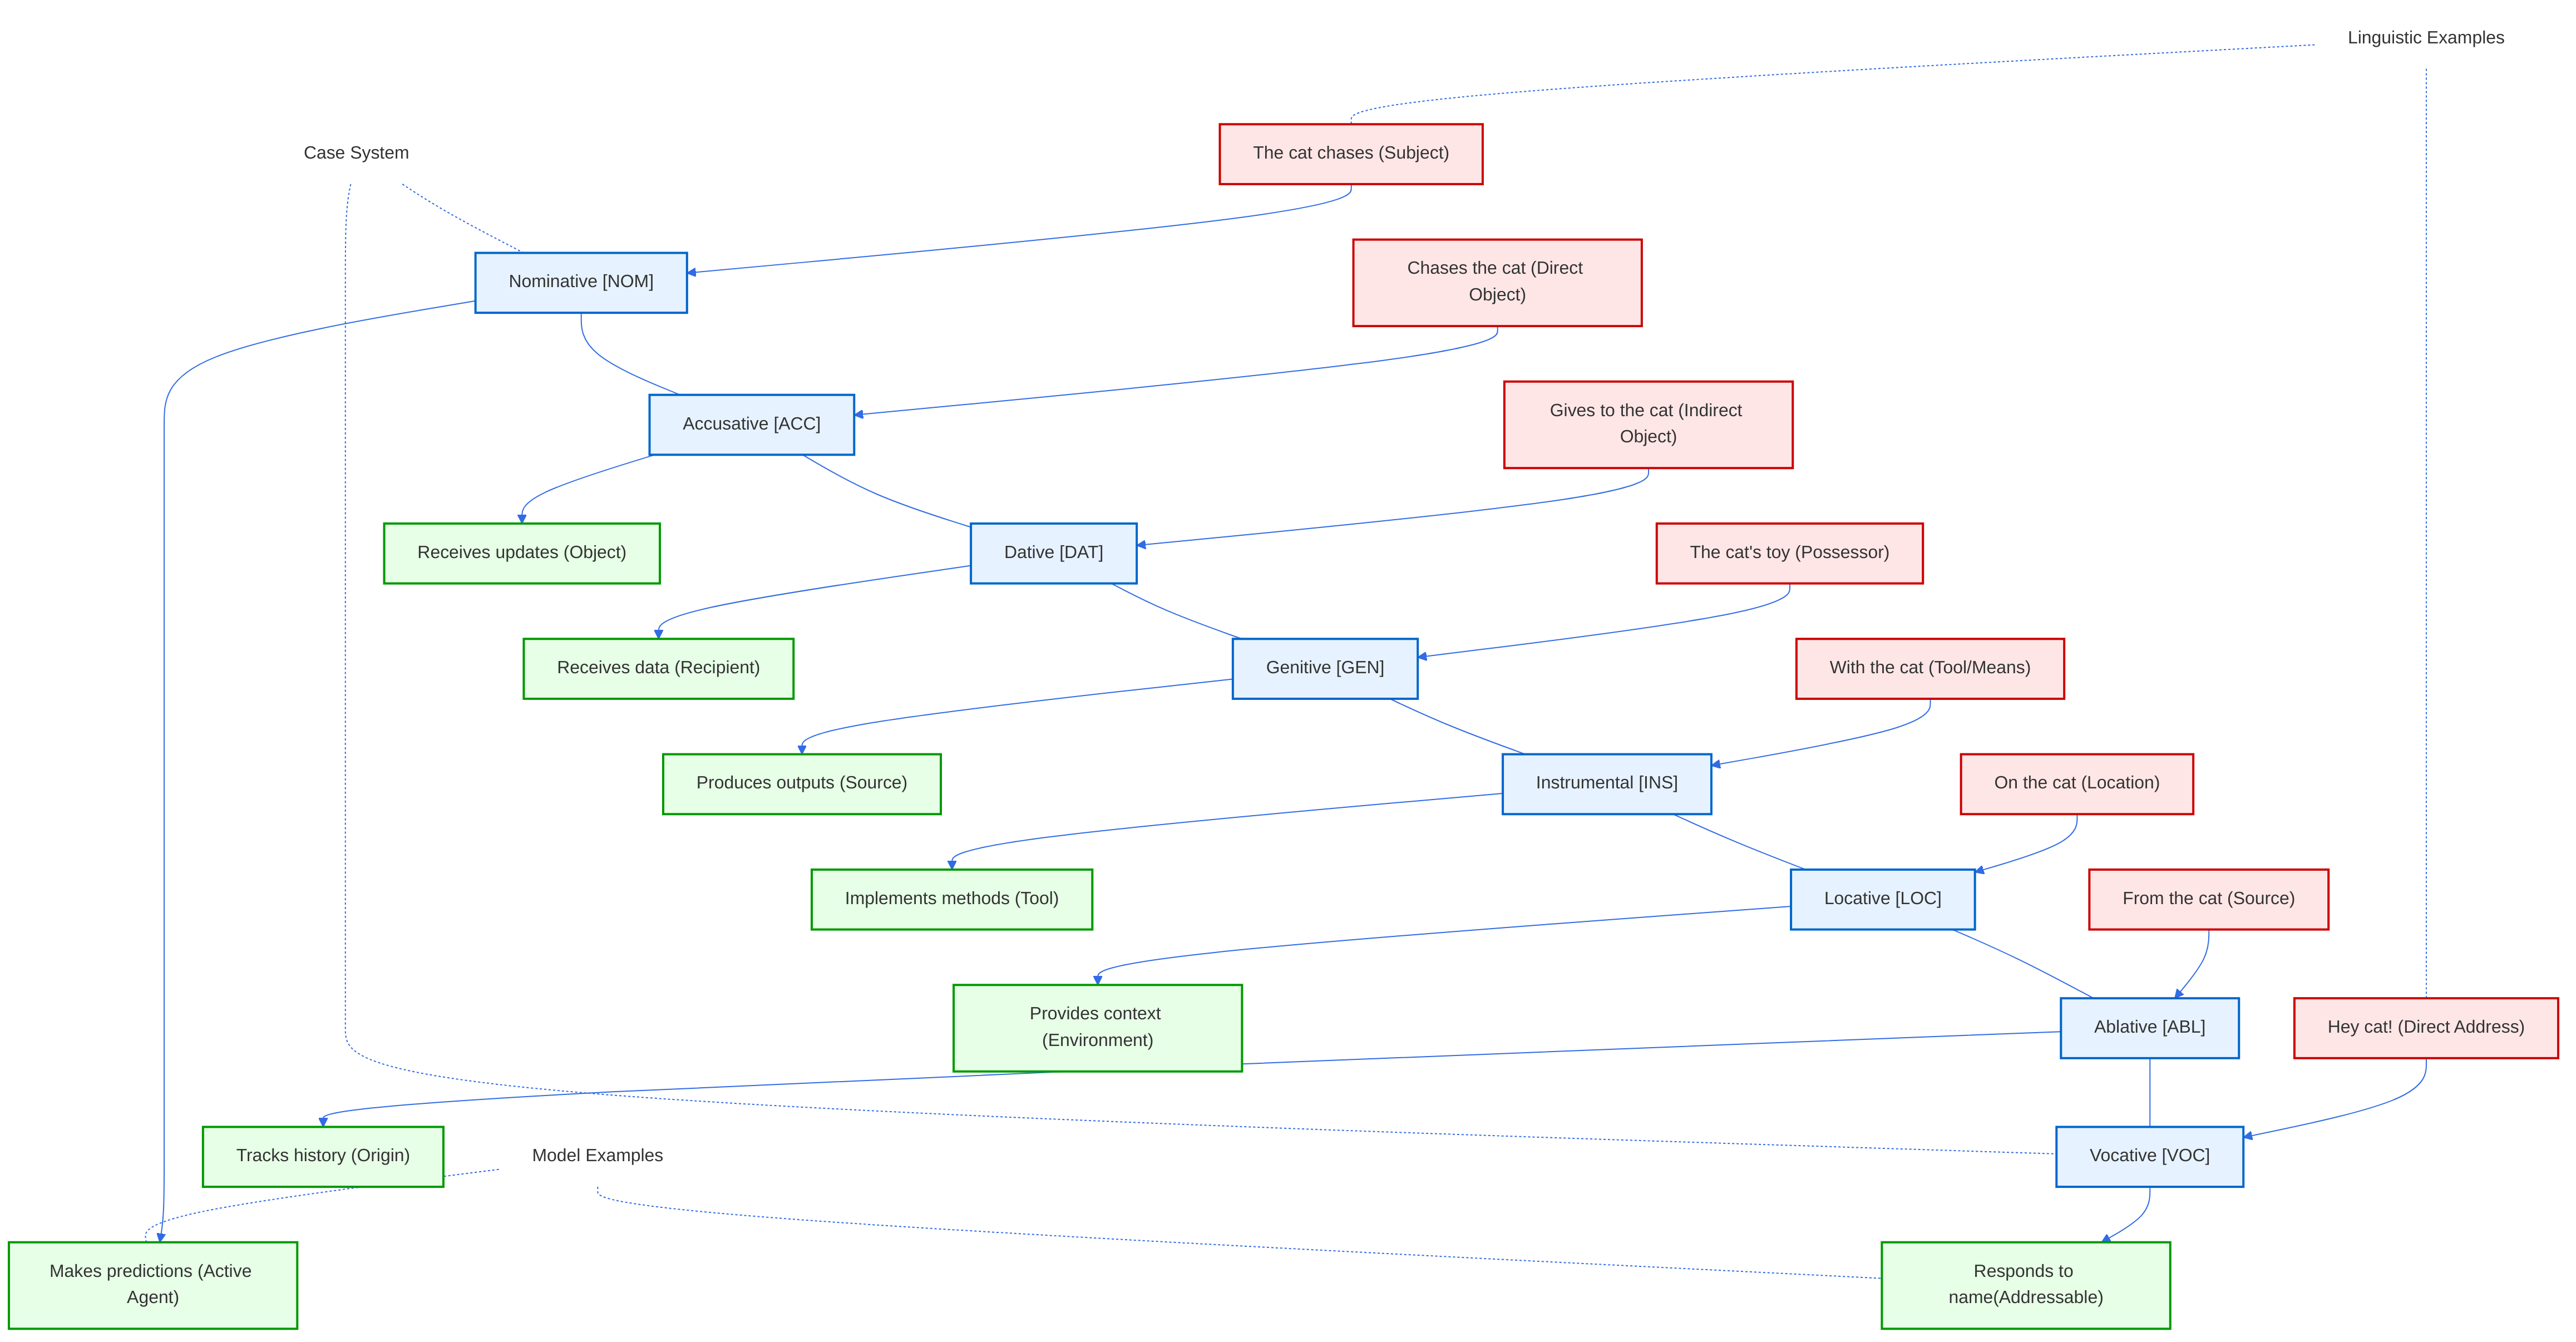
\includegraphics{figures/Figure_2.png}
\caption{Figure 2: illustrates this linguistic parallel}
\end{figure}

\includegraphics{\#figure-2-illustrates-this-linguistic-parallel}(f

{[}Figure 3: Figure 3{]}(figures/Figure\_3{]}(figures/Figure\_3.png)

{[}Figure 3: Figure
3{]}(figures/Figure\_3{]}(figures/Figure\_3.png){]}(figures/Figure\_3.png)

igures/Figure\_2.p

\begin{figure}
\centering
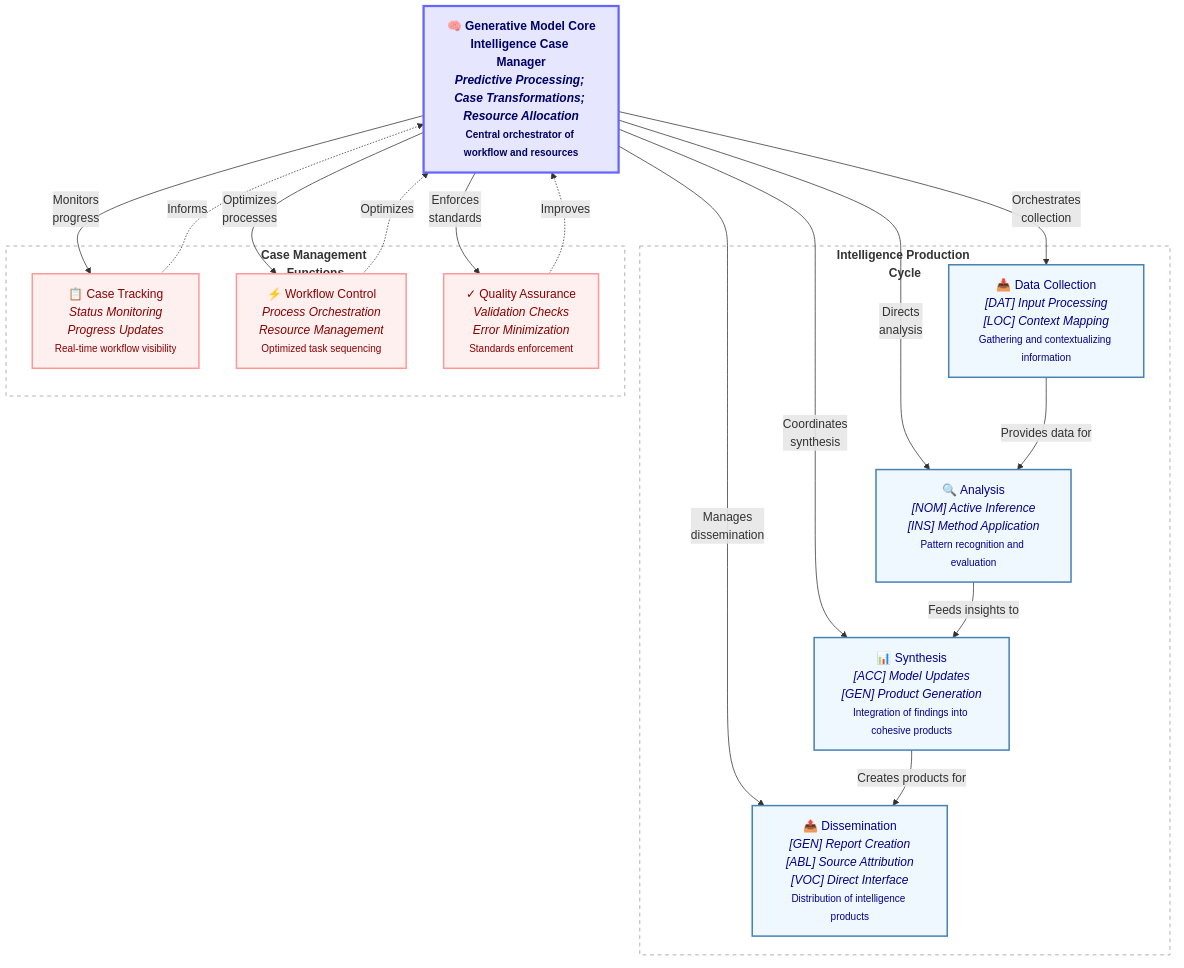
\includegraphics{figures/Figure_4.png}
\caption{Figure 4: illustrates how this core framework integrates with
intelligence case management}
\end{figure}

\begin{figure}
\centering
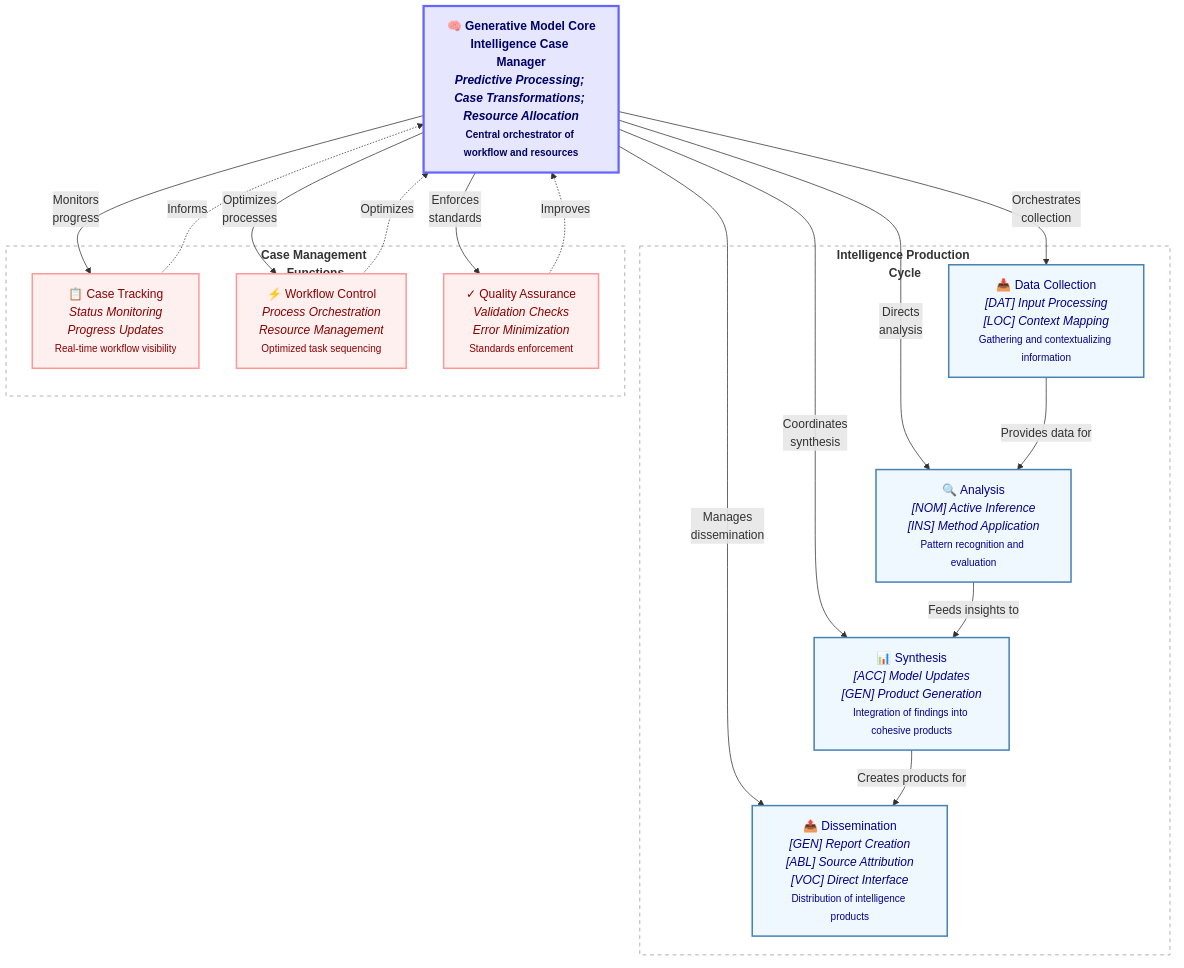
\includegraphics{figures/Figure_4.png}
\caption{Figure 4: illustrates how this core framework integrates with
intelligence case management}
\end{figure}

{[}Figure 5: provides a sequence diagram of a typical transformation
cycle, and Figur{]}(figures/Figure\_5{]}(figures/Figure\_5.png)

!{[}Figure 5: provides a sequence diagram of a

{[}Figure 6: s{]}(figures/Figure\_6{]}(figures/Figure\_6.png)

{[}Figure 6:
s{]}(figures/Figure\_6{]}(figures/Figure\_6.png){]}(figures/Figure\_6.png)

typical transformation cycle, and
Figur{]}(figures/Figure\_5{]}(figures/Figure\_5.png){]}(figures/Figure

\begin{figure}
\centering
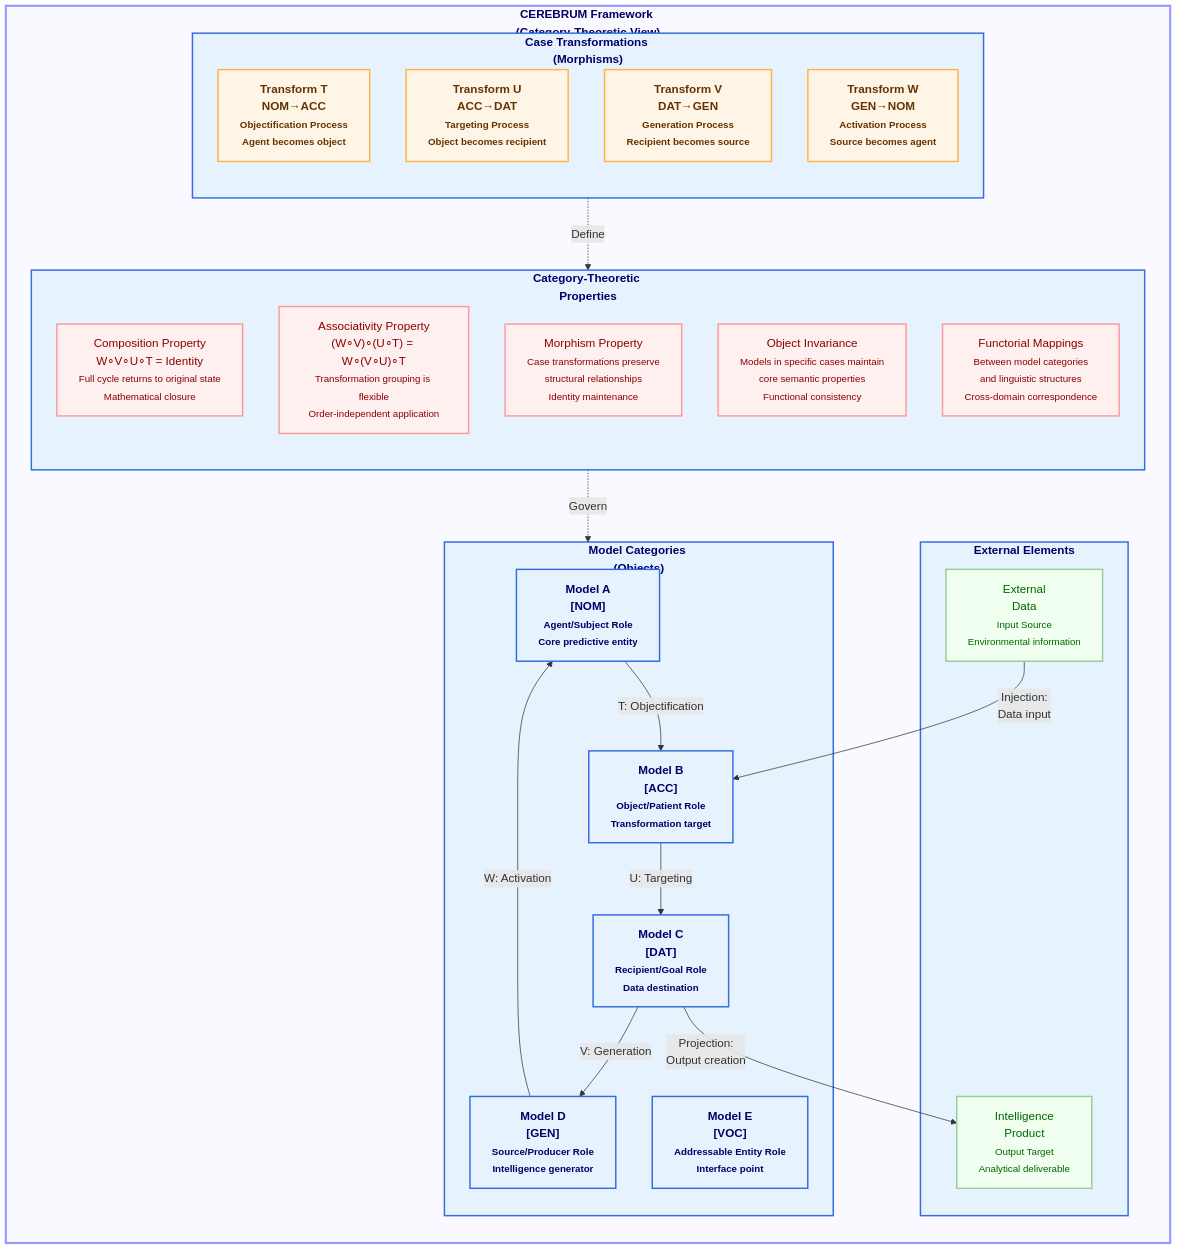
\includegraphics{figures/Figure_7.png}
\caption{Figure 7: CEREBRUM Category Theory Framework. Demonstrates the
category-theoretic formalization of case relationships and
transformations between cognitive models.}
\end{figure}

!{[}Figure 7: CEREBRUM Category Theory Framework. Dem

{[}Figure 8: Figure 8{]}(figures/Figure\_8{]}(figures/Figure\_8.png)

{[}Figure 8: Figure 8{]}(figures/Figure\_8{]}(figures/Fig

{[}Figure 9: Figure 9{]}(figures/Figure\_9{]}(figures/Figure\_9.png)

{[}Figure 9: Figure
9{]}(figures/Figure\_9{]}(figures/Figure\_9.png){]}(figures/Figure

{[}Figure 10: demonstrates the practical
imple{]}(figures/Figure\_10{]}(figures/Figure\_10.png)

{[}Figure 10: demonstrates the practical
imple{]}(figures/Figure\_10{]}(figures/Figure\_10.png){]}(figures/Figure\_

\begin{figure}
\centering
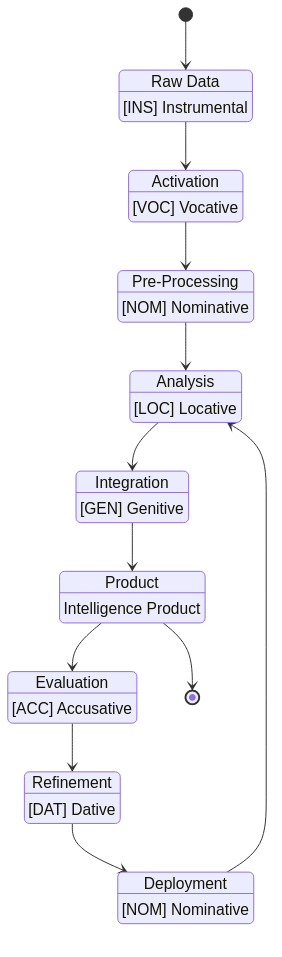
\includegraphics{figures/Figure_11.png}
\caption{Figure 11: and Figure 12 provide alternative state-based
visualizations of these workflows}
\end{figure}

!{[}Figure 11: and Figure 12 provide alternative state-based
visualizations of these workflow

\begin{figure}
\centering
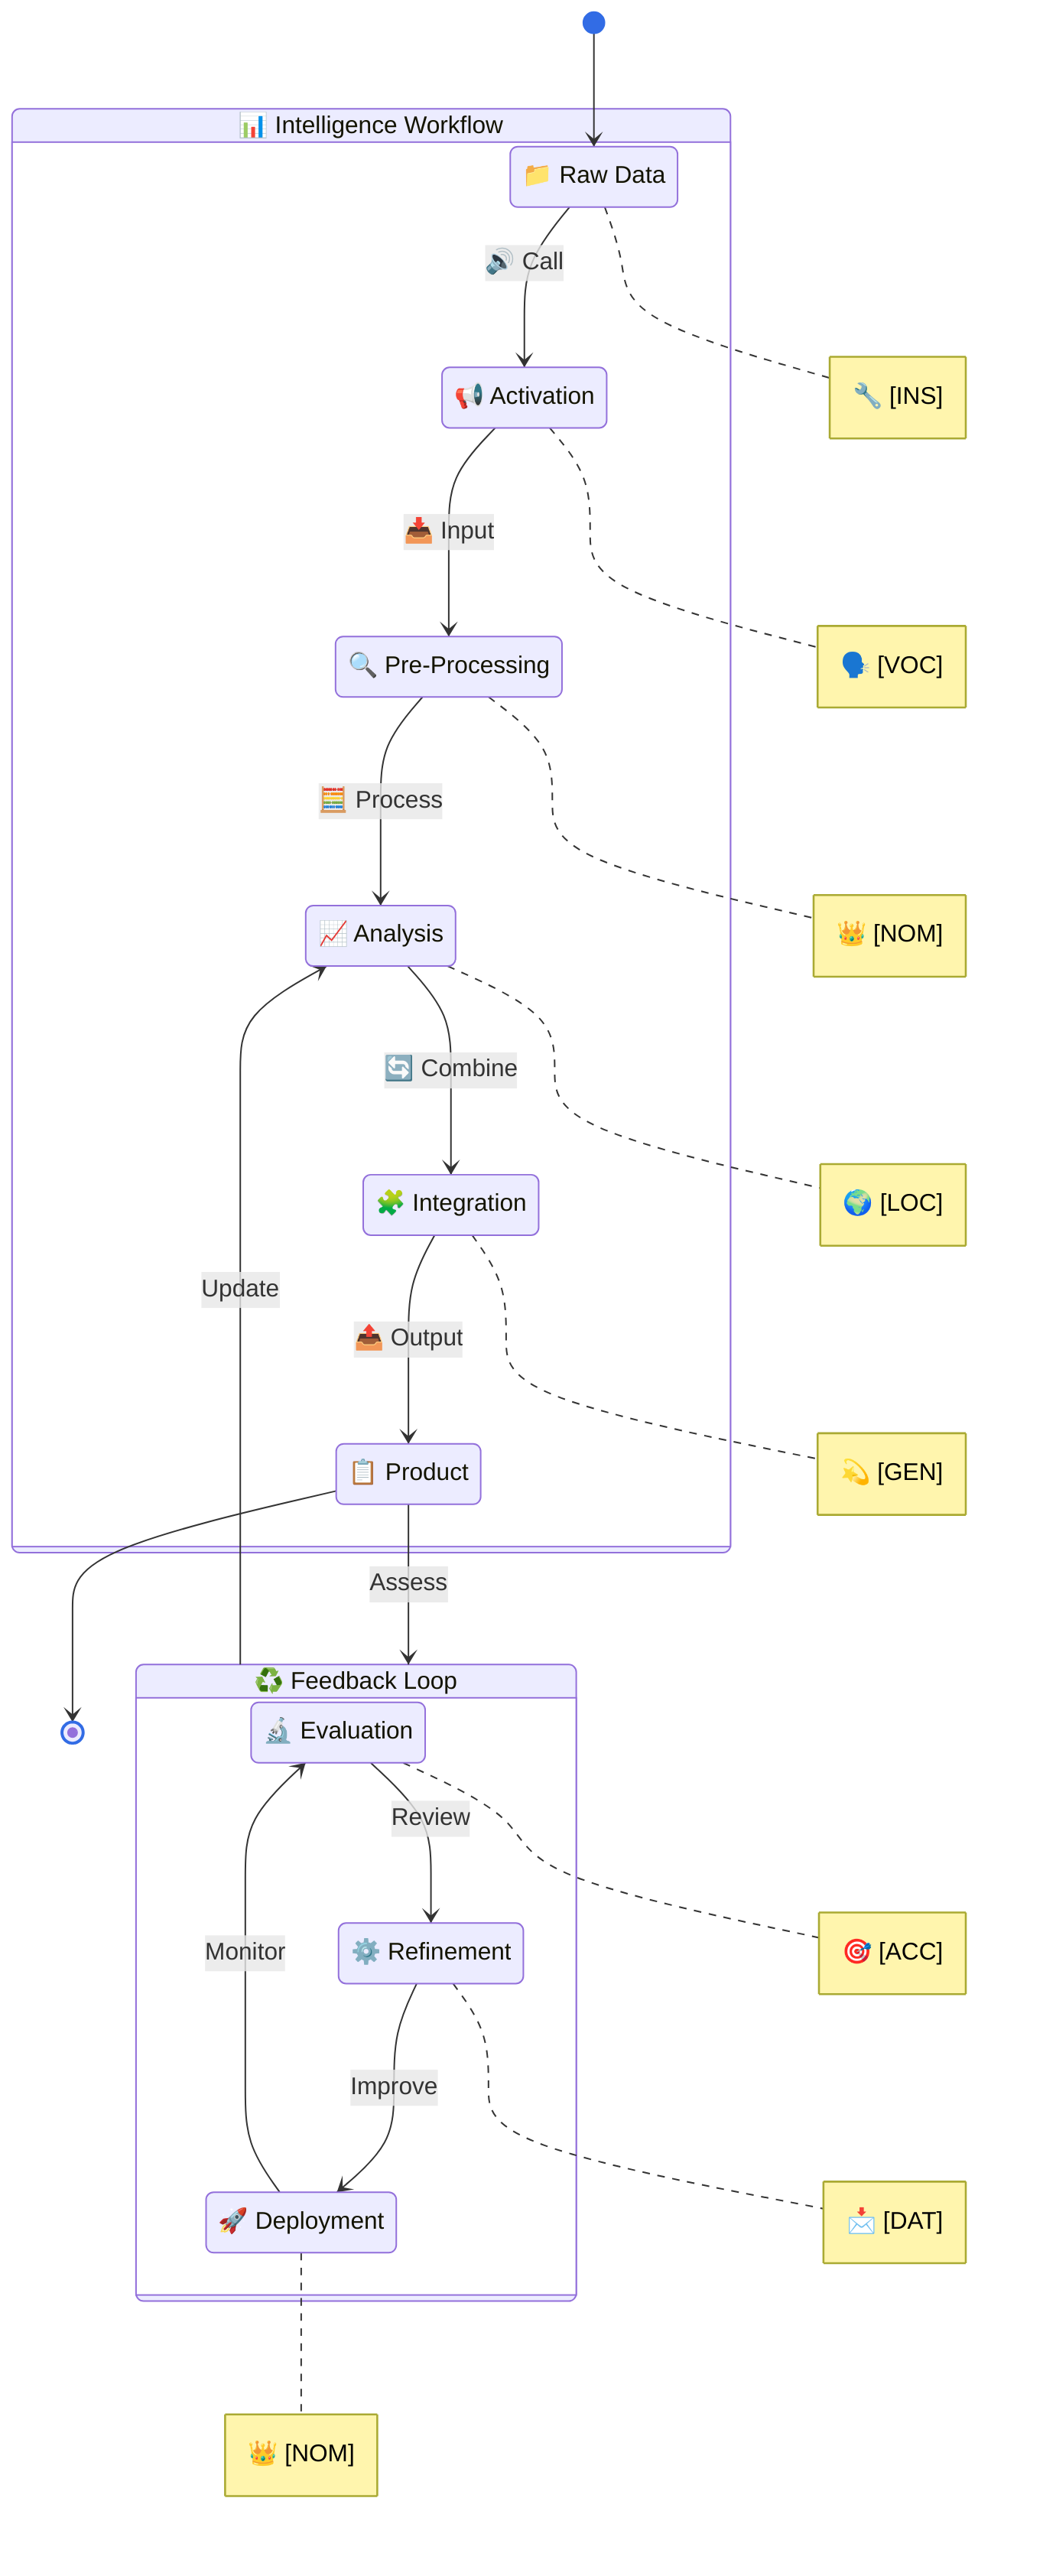
\includegraphics{figures/Figure_12.png}
\caption{Figure 12: provide alternative state-based visualizations of
these workflows}
\end{figure}

!{[}Figure 12: provide alternative state-based visualiza

{[}Figure 13: Figure 13{]}(figures/Figure\_13{]}(figures/Figure\_13.png)

{[}Figure 13: Figure
13{]}(figures/Figure\_13{]}(figures/Figure\_13.png){]}(fig

\begin{figure}
\centering
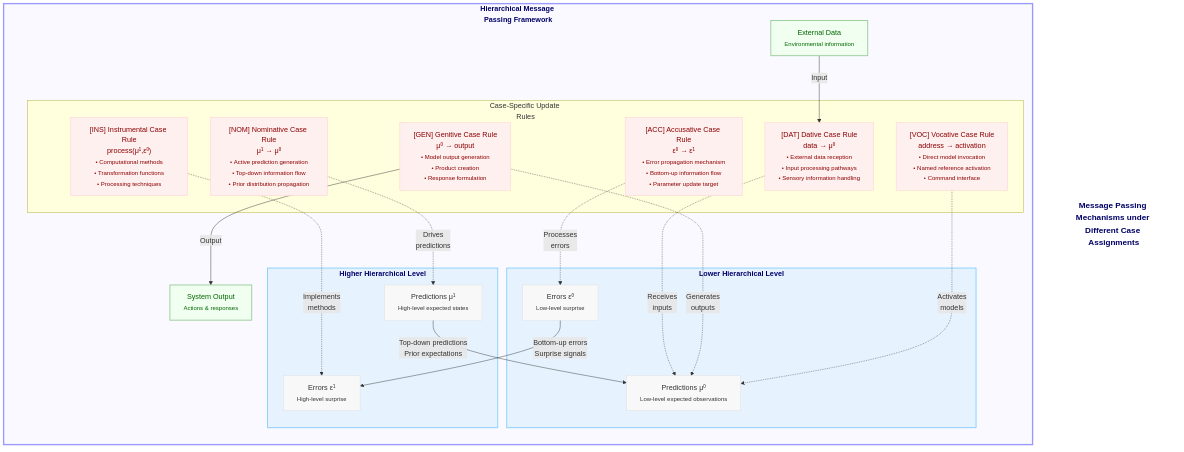
\includegraphics{figures/Figure_14.png}
\caption{Figure 14: details the associated message passing rules}
\end{figure}

!{[}Figure 14: details the associated message passing ru

{[}Figure 15: Figure 15{]}(figures/Figure\_15{]}(figures/Figure\_15.png)

{[}Figure 15: Figure
15{]}(figures/Figure\_15{]}(figures/Figure\_15.png){]}(figures/Figure\_15.png)

les{]}(figures/Figure\_14.png){]}(figures/Figure\_14.png)

ures/Figure\_13.png)

tions of these
workflows{]}(figures/Figure\_12.png){]}(figures/Figure\_12.png)

s{]}(figures/Figure\_11.png){]}(figures/Figure\_11.png)

10.png)

\_9.png)

ure\_8.png){]}(figures/Figure\_8.png)

onstrates the category-theoretic formalization of case relationships and
transformations between cognitive
models.{]}(figures/Figure\_7.png){]}(figures/Figure\_7.png)

\_5.png)

{]}(figures/Figure\_4.png)

ng){]}(figures/Figure\_2.png)

{]}(figures/Figure\_1.png)

\pagebreak

\hypertarget{figure-2-illustrates-this-linguistic-parallel}{%
\subsection{Figure 2: illustrates this linguistic
parallel}\label{figure-2-illustrates-this-linguistic-parallel}}

\begin{figure}
\centering
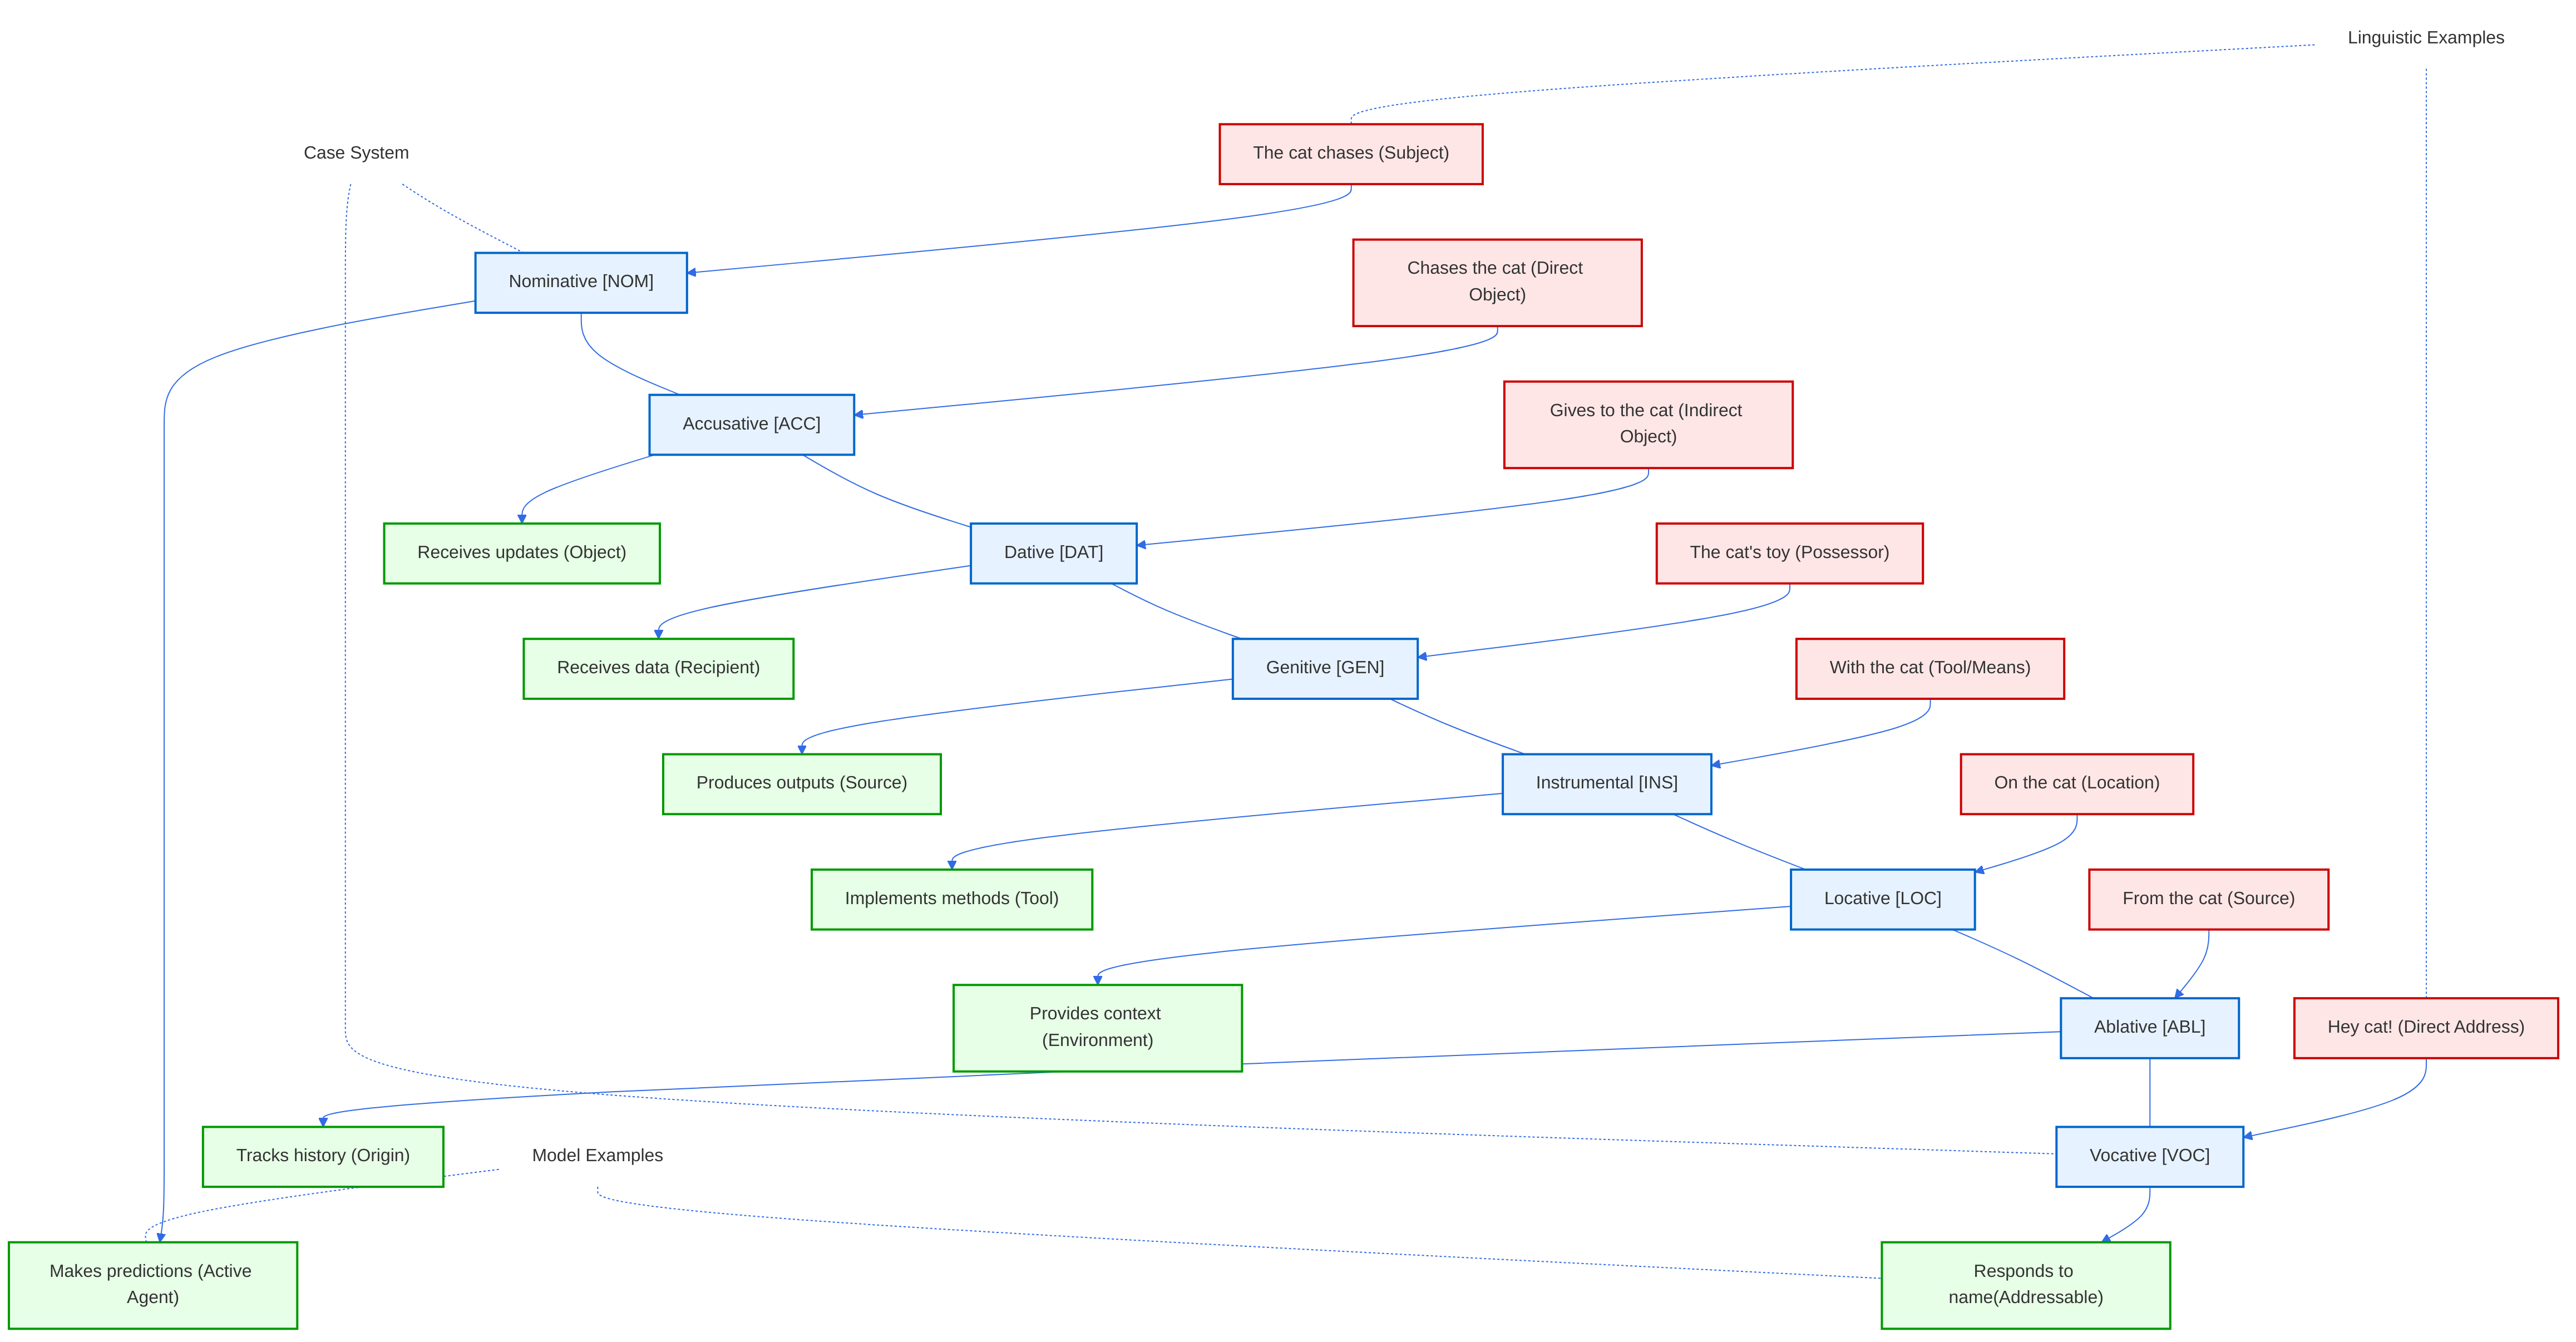
\includegraphics{figures/Figure_2.png}
\caption{Figure 2: illustrates this linguistic parallel}
\end{figure}

\pagebreak

\hypertarget{figure-3-figure-3figuresfigure_3}{%
\subsection{Figure 3: Figure
3{]}(figures/Figure\_3}\label{figure-3-figure-3figuresfigure_3}}

{[}Figure 3: Figure 3{]}(figures/Figure\_3{]}(figures/Figure\_3.png)

\pagebreak

\hypertarget{figure-4-illustrates-how-this-core-framework-integrates-with-intelligence-case-management}{%
\subsection{Figure 4: illustrates how this core framework integrates
with intelligence case
management}\label{figure-4-illustrates-how-this-core-framework-integrates-with-intelligence-case-management}}

\begin{figure}
\centering
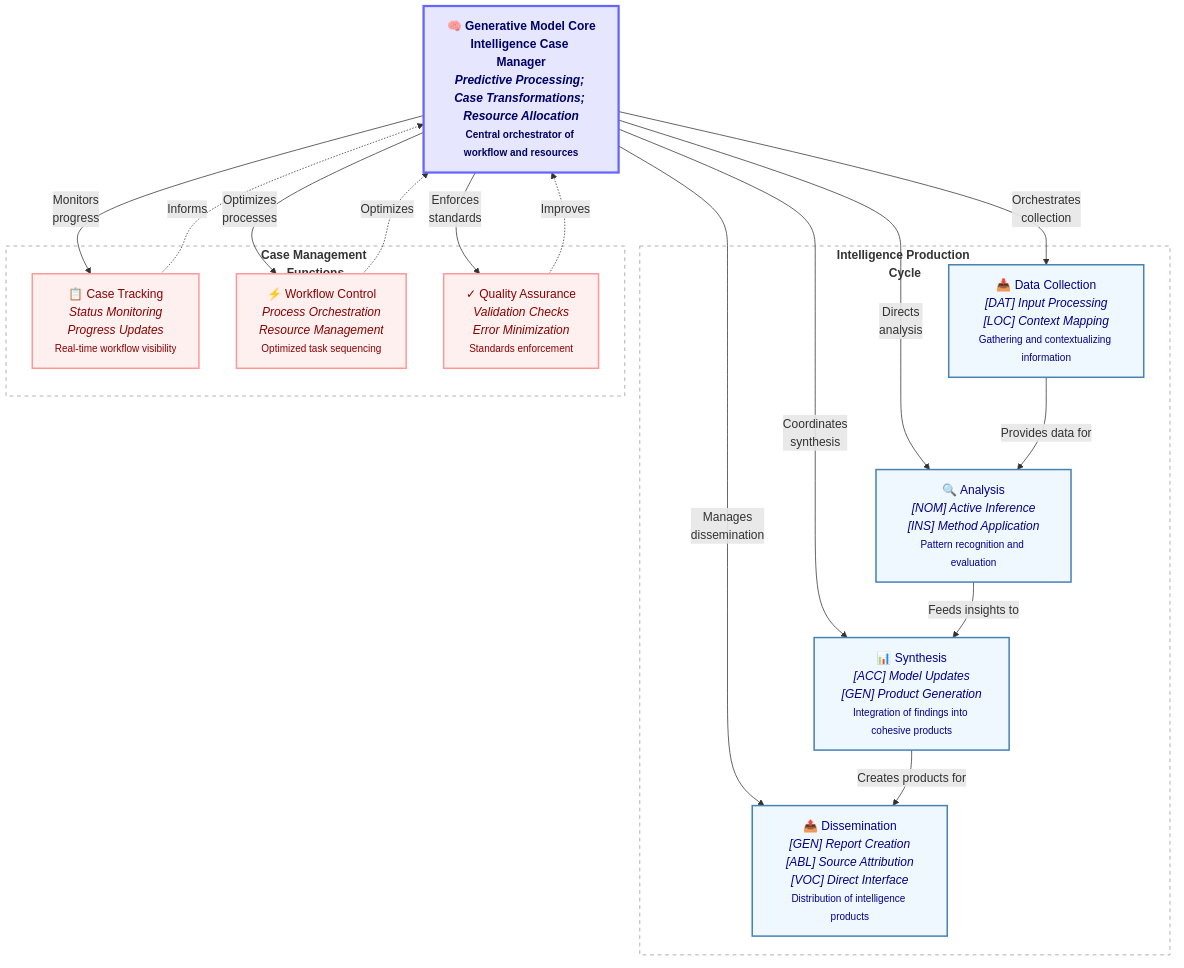
\includegraphics{figures/Figure_4.png}
\caption{Figure 4: illustrates how this core framework integrates with
intelligence case management}
\end{figure}

\pagebreak

\hypertarget{figure-5-provides-a-sequence-diagram-of-a-typical-transformation-cycle-and-figurfiguresfigure_5}{%
\subsection{Figure 5: provides a sequence diagram of a typical
transformation cycle, and
Figur{]}(figures/Figure\_5}\label{figure-5-provides-a-sequence-diagram-of-a-typical-transformation-cycle-and-figurfiguresfigure_5}}

{[}Figure 5: provides a sequence diagram of a typical transformation
cycle, and Figur{]}(figures/Figure\_5{]}(figures/Figure\_5.png)

\pagebreak

\hypertarget{figure-6-sfiguresfigure_6}{%
\subsection{Figure 6:
s{]}(figures/Figure\_6}\label{figure-6-sfiguresfigure_6}}

{[}Figure 6: s{]}(figures/Figure\_6{]}(figures/Figure\_6.png)

\pagebreak

\hypertarget{figure-7-cerebrum-category-theory-framework.-demonstrates-the-category-theoretic-formalization-of-case-relationships-and-transformations-between-cognitive-models.}{%
\subsection{Figure 7: CEREBRUM Category Theory Framework. Demonstrates
the category-theoretic formalization of case relationships and
transformations between cognitive
models.}\label{figure-7-cerebrum-category-theory-framework.-demonstrates-the-category-theoretic-formalization-of-case-relationships-and-transformations-between-cognitive-models.}}

\begin{figure}
\centering
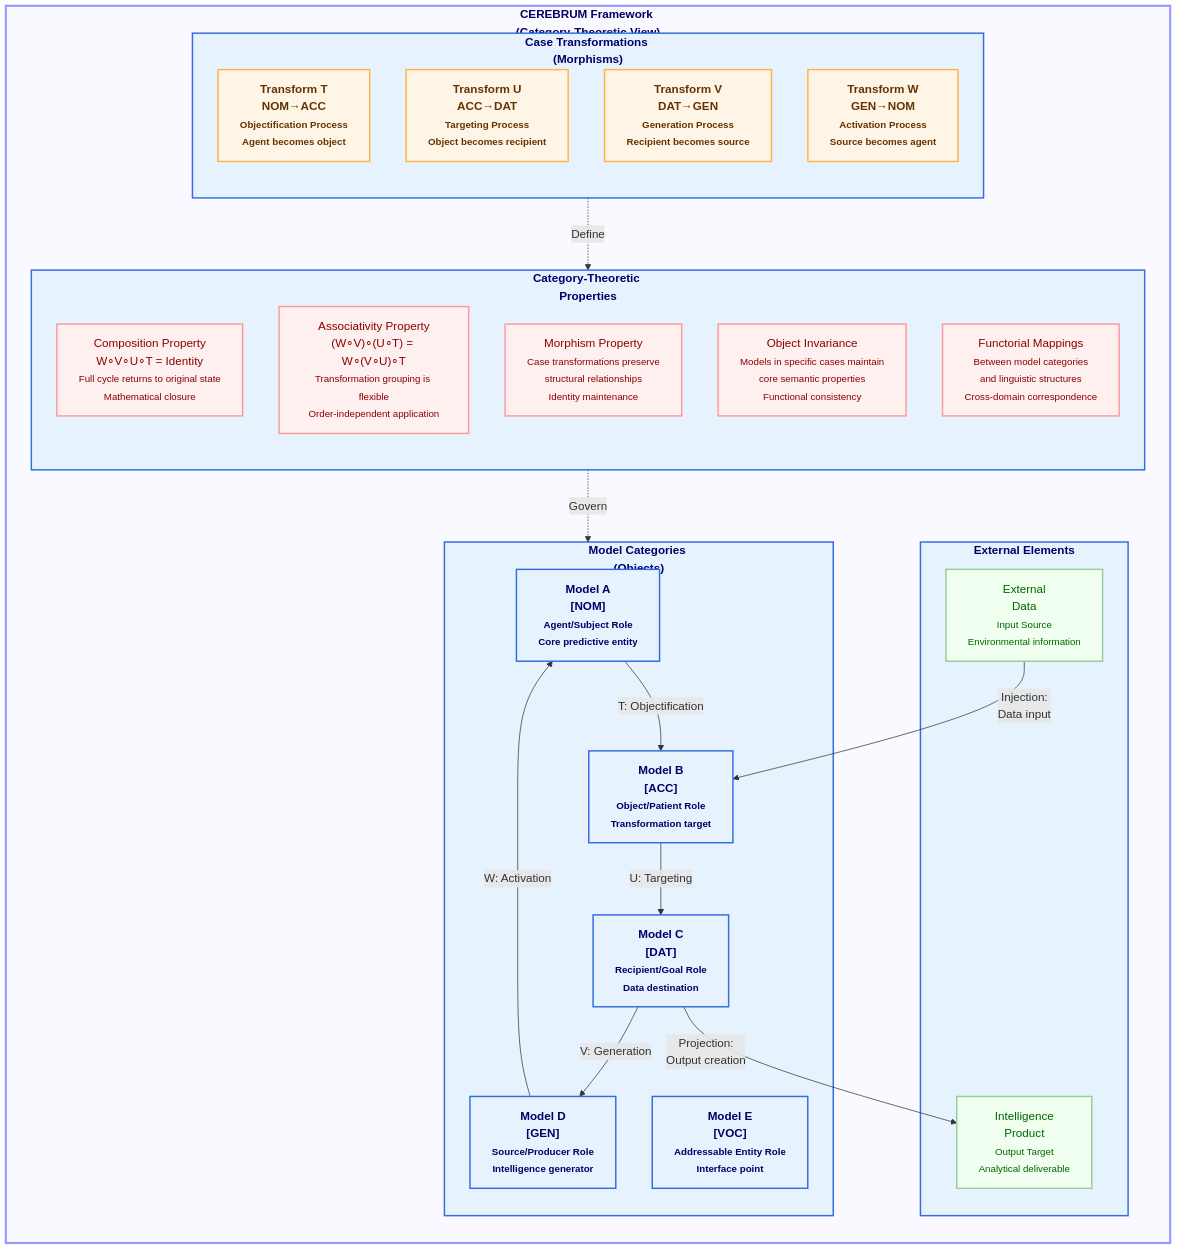
\includegraphics{figures/Figure_7.png}
\caption{Figure 7: CEREBRUM Category Theory Framework. Demonstrates the
category-theoretic formalization of case relationships and
transformations between cognitive models.}
\end{figure}

\pagebreak

\hypertarget{figure-8-figure-8figuresfigure_8}{%
\subsection{Figure 8: Figure
8{]}(figures/Figure\_8}\label{figure-8-figure-8figuresfigure_8}}

{[}Figure 8: Figure 8{]}(figures/Figure\_8{]}(figures/Figure\_8.png)

\pagebreak

\hypertarget{figure-9-figure-9figuresfigure_9}{%
\subsection{Figure 9: Figure
9{]}(figures/Figure\_9}\label{figure-9-figure-9figuresfigure_9}}

{[}Figure 9: Figure 9{]}(figures/Figure\_9{]}(figures/Figure\_9.png)

\pagebreak

\hypertarget{figure-10-demonstrates-the-practical-implefiguresfigure_10}{%
\subsection{Figure 10: demonstrates the practical
imple{]}(figures/Figure\_10}\label{figure-10-demonstrates-the-practical-implefiguresfigure_10}}

{[}Figure 10: demonstrates the practical
imple{]}(figures/Figure\_10{]}(figures/Figure\_10.png)

\pagebreak

\hypertarget{figure-11-and-figure-12-provide-alternative-state-based-visualizations-of-these-workflows}{%
\subsection{Figure 11: and Figure 12 provide alternative state-based
visualizations of these
workflows}\label{figure-11-and-figure-12-provide-alternative-state-based-visualizations-of-these-workflows}}

\begin{figure}
\centering
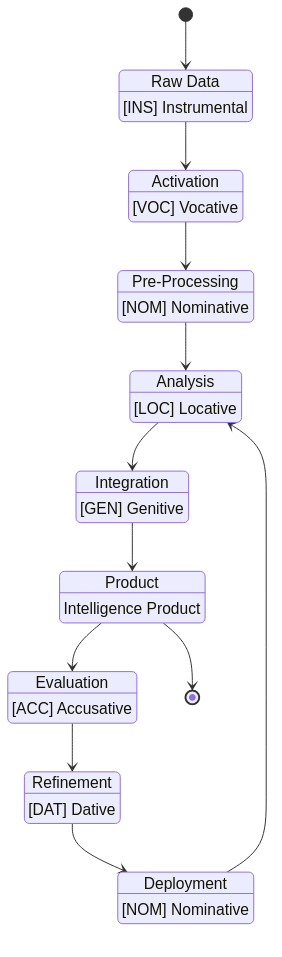
\includegraphics{figures/Figure_11.png}
\caption{Figure 11: and Figure 12 provide alternative state-based
visualizations of these workflows}
\end{figure}

\pagebreak

\hypertarget{figure-12-provide-alternative-state-based-visualizations-of-these-workflows}{%
\subsection{Figure 12: provide alternative state-based visualizations of
these
workflows}\label{figure-12-provide-alternative-state-based-visualizations-of-these-workflows}}

\begin{figure}
\centering
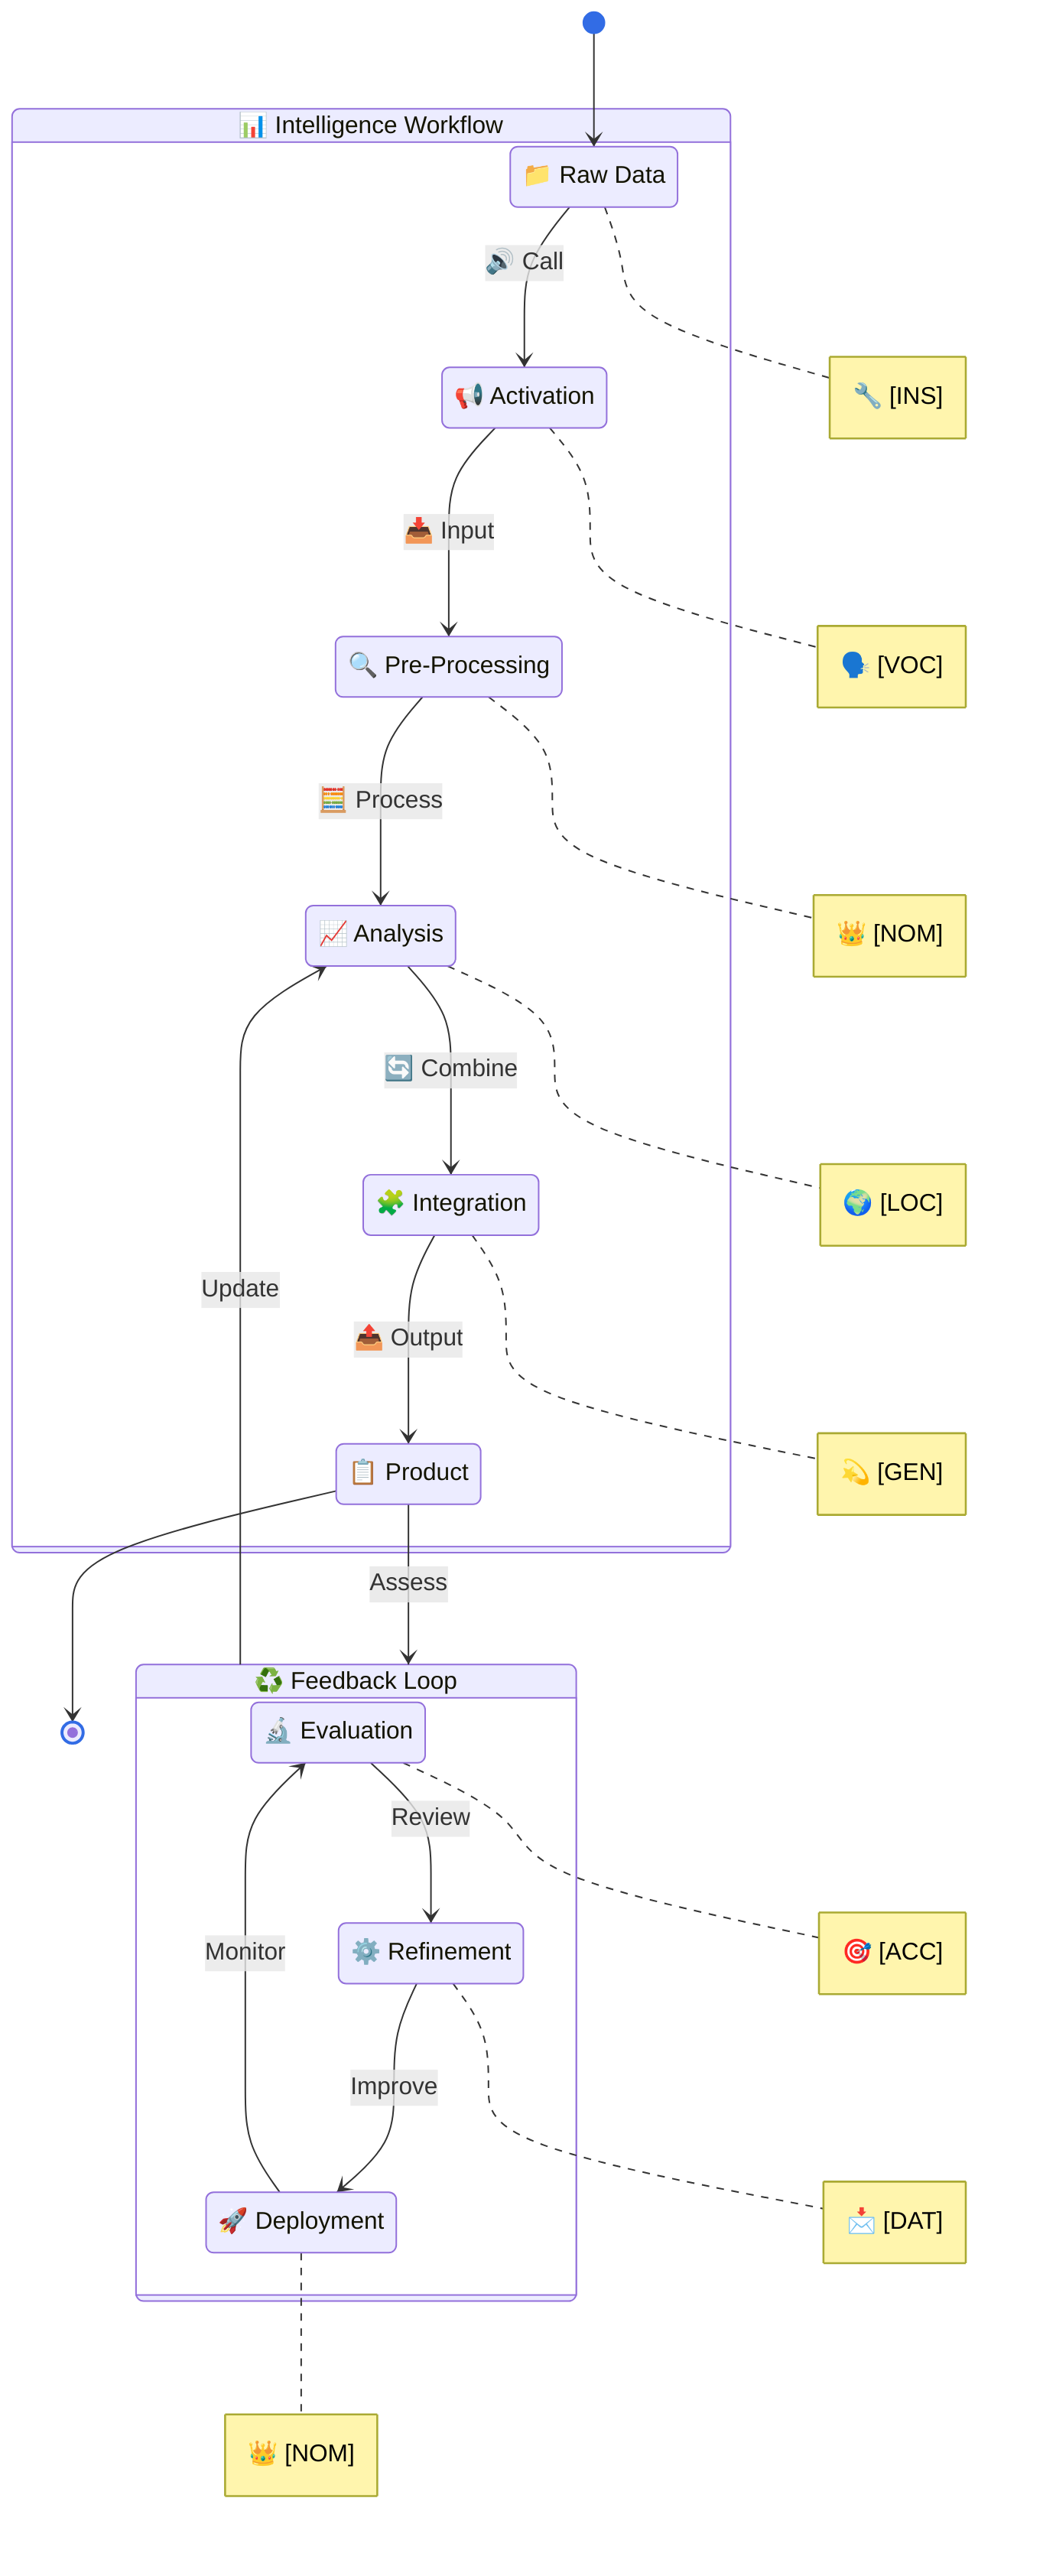
\includegraphics{figures/Figure_12.png}
\caption{Figure 12: provide alternative state-based visualizations of
these workflows}
\end{figure}

\pagebreak

\hypertarget{figure-13-figure-13figuresfigure_13}{%
\subsection{Figure 13: Figure
13{]}(figures/Figure\_13}\label{figure-13-figure-13figuresfigure_13}}

{[}Figure 13: Figure 13{]}(figures/Figure\_13{]}(figures/Figure\_13.png)

\pagebreak

\hypertarget{figure-14-details-the-associated-message-passing-rules}{%
\subsection{Figure 14: details the associated message passing
rules}\label{figure-14-details-the-associated-message-passing-rules}}

\begin{figure}
\centering
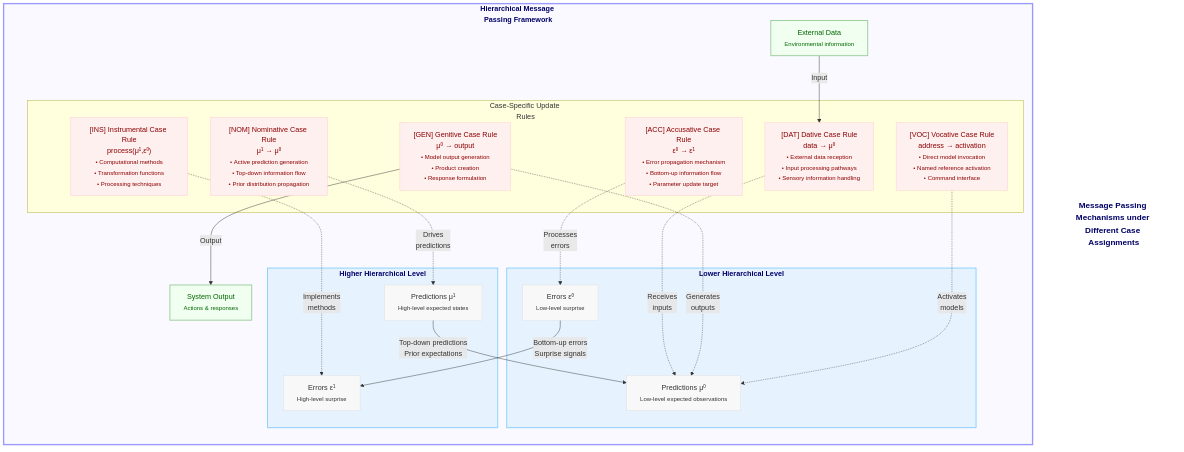
\includegraphics{figures/Figure_14.png}
\caption{Figure 14: details the associated message passing rules}
\end{figure}

\pagebreak

\hypertarget{figure-15-figure-15figuresfigure_15}{%
\subsection{Figure 15: Figure
15{]}(figures/Figure\_15}\label{figure-15-figure-15figuresfigure_15}}

{[}Figure 15: Figure 15{]}(figures/Figure\_15{]}(figures/Figure\_15.png)

\pagebreak

\hypertarget{mathematical-formalization}{%
\section{Mathematical Formalization}\label{mathematical-formalization}}

This supplement contains all mathematical formalizations referenced
throughout the paper, organized by equation number.

\hypertarget{variational-free-energy-and-case-transformations}{%
\subsection{Variational Free Energy and Case
Transformations}\label{variational-free-energy-and-case-transformations}}

\textbf{Equation 1: Variational Free Energy for Case Transformation}

\[
F = D_{KL}[q(s|T(m))||p(s|m)] - \mathbb{E}_{p}[\log p(o|s,T(m))]  \tag{1}
\]

where T(m) represents the transformed model, s are internal states, and
o are observations.

\textbf{Equation 2: Markov Blanket and Case Relationship}

\[\text{Case}(M) \subseteq \text{MB}(M)  \tag{2}\]

where MB(M) denotes the Markov blanket of model M.

\textbf{Equation 3: Precision Weighting for Case Selection}

\[\beta(c,m) = \frac{\exp(-F(c,m))}{\sum_{i}\exp(-F(c_i,m))}  \tag{3}\]

where (c,m) is the precision weight for case c and model m.

\textbf{Equation 4: Case-Specific Gradient Descent on Free Energy}

\[\frac{\partial m}{\partial t} = -\kappa_c \cdot \frac{\partial F}{\partial m}  \tag{4}\]

where \(\kappa_c\) is the case-specific learning rate.

\textbf{Equation 5: Expected Free Energy Reduction in Case Transitions}

\[
\mathbb{E}[\Delta F] = \sum_{s,a}T(s'|s,a)\pi[a|s](F(s,c)-F(s',c'))  \tag{5}
\]

where c and c' represent the initial and target cases respectively.

\textbf{Equation 6: Bayes Factor for Case Selection}

\[BF = \frac{p(o|m,c_1)}{p(o|m,c_2)}  \tag{6}\]

\textbf{Equation 7: Free Energy Minimization in Case Transitions}

\[
F = D_{KL}[q(s|c,m) || p(s|m)] - \mathbb{E}_{q(s|c,m)}[\log p(o|s,c,m)]  \tag{7}
\]

\hypertarget{message-passing-rules-for-different-cases}{%
\subsection{Message Passing Rules for Different
Cases}\label{message-passing-rules-for-different-cases}}

These equations illustrate how case assignments modulate standard
hierarchical message passing (e.g., in predictive coding) where
beliefs/predictions (\(\mu\)) and prediction errors (\(\varepsilon\))
flow between adjacent levels (denoted by superscripts 0 and 1). The
case-specific weights (\(\kappa_c\)) determine the influence of each
message type based on the model's current functional role.

\textbf{Equations 8-12: Case-Specific Message Passing Rules}

\[\text{Nominative [NOM]}: \mu^0 = \mu^0 + \kappa_{NOM} \cdot (\mu^1 - \mu^0)  \tag{8}\]
\emph{(Lower-level prediction \(\mu^0\) updated by top-down prediction
\(\mu^1\), weighted by \(\kappa_{NOM}\))}

\[\text{Accusative [ACC]}: \varepsilon^1 = \varepsilon^1 + \kappa_{ACC} \cdot (\varepsilon^0 - \varepsilon^1)  \tag{9}\]
\emph{(Higher-level error \(\varepsilon^1\) updated by bottom-up error
\(\varepsilon^0\), weighted by \(\kappa_{ACC}\))}

\[\text{Dative [DAT]}: \mu^0 = \mu^0 + \kappa_{DAT} \cdot (data - \mu^0)  \tag{10}\]
\emph{(Lower-level prediction \(\mu^0\) updated directly by incoming
`data', weighted by \(\kappa_{DAT}\))}

\[\text{Genitive [GEN]}: output = \mu^0 + \kappa_{GEN} \cdot \eta  \tag{11}\]
\emph{(Output generated based on lower-level prediction \(\mu^0\),
weighted by \(\kappa_{GEN}\), potentially with noise \(\eta\))}

\[\text{Instrumental [INS]}: process = f(\mu^1, \varepsilon^0) \cdot \kappa_{INS} \tag{12}\]

\emph{(A process output determined by some function \(f\) of top-down
prediction \(\mu^1\) and bottom-up error \(\varepsilon^0\), weighted by
\(\kappa_{INS}\))}

\[\text{Vocative [VOC]}: activation = \sigma(\kappa_{VOC} \cdot sim(id, address)) \tag{12a}\]

\emph{(Activation state determined by similarity between model identity
\(id\) and incoming address, weighted by \(\kappa_{VOC}\) and passed
through activation function \(\sigma\))}

where \(\kappa_c\) represents case-specific learning rates or precision
weights, \(\eta\) is a noise term, \(\mu^0, \mu^1\) represent
beliefs/predictions, and \(\varepsilon^0, \varepsilon^1\) represent
prediction errors at adjacent hierarchical levels.

\hypertarget{precision-allocation-and-resource-optimization}{%
\subsection{Precision Allocation and Resource
Optimization}\label{precision-allocation-and-resource-optimization}}

\textbf{Equation 13: Precision Weight Allocation with Temperature}

\[\beta(c,m) = \frac{\exp(-\gamma \cdot F(c,m))}{\sum_i \exp(-\gamma \cdot F(c_i,m))}  \tag{13}\]

where is the inverse temperature parameter controlling allocation
sharpness.

\textbf{Equation 14: Resource-Weighted Free Energy}

\[F_{\beta}(m) = \sum_c \beta(c,m) \cdot F(c,m) \cdot R(c)  \tag{14}\]

where R(c) represents the computational resources allocated to case c.

\hypertarget{novel-case-formalizations}{%
\subsection{Novel Case Formalizations}\label{novel-case-formalizations}}

\textbf{Equation 15: Conjunctive Case Free Energy}

\[
F_{CNJ} = D_{KL}[q(s|CNJ,m) || p(s|m)] - \mathbb{E}_{q(s|CNJ,m)}[\log p(o|s,\{m_i\})]  \tag{15}
\]

where \{m\_i\} represents the assembly of connected models.

\textbf{Equation 16: Conjunctive Case Message Passing}

\[\mu^{CNJ} = \sum_i w_i \cdot \mu_i + \kappa_{CNJ} \cdot (\prod_i \mu_i - \sum_i w_i \cdot \mu_i)  \tag{16}\]

where w\_i are model-specific weighting factors.

\textbf{Equation 17: Recursive Case Precision Dynamics}

\[\beta(REC,m) = \frac{\exp(-\gamma \cdot F(REC,m))}{\sum_i \exp(-\gamma \cdot F(c_i,m)) + \exp(-\gamma \cdot F(REC,m))}  \tag{17}\]

\hypertarget{glossary-of-variables}{%
\subsection{Glossary of Variables}\label{glossary-of-variables}}

\begin{itemize}
\tightlist
\item
  \(a\): Action (in MDP context, often selecting a case transition)
\item
  \(\alpha\): Learning rate (in Neural Process Models context)
\item
  \(BF\): Bayes Factor (for comparing model evidence between cases)
\item
  \(c, c_i, c', c_1, c_2\): Linguistic case assignment (e.g., NOM, ACC,
  specific case instances)
\item
  \(\text{Case}(M)\): Case assignment of model \(M\)
\item
  \textbf{Case Transformation}: An operation that changes the functional
  role (case) of a model within the system
\item
  \textbf{CEREBRUM}: Case-Enabled Reasoning Engine with Bayesian
  Representations for Unified Modeling
\item
  \(D_{KL}\): Kullback-Leibler divergence
\item
  \(\text{data}\): Input data (in Dative case message passing; Eq 10)
\item
  \textbf{Declinability}: The capacity of a generative model within
  CEREBRUM to assume different morphological and functional roles
  (cases) through transformations
\item
  \(E_p[\cdot]\): Expectation with respect to distribution \(p\)
  (Information Geometry)
\item
  \(\mathbb{E}[\cdot]\): Expectation operator
\item
  \(F\): Variational Free Energy
\item
  \(F_{\beta}(m)\): Resource-weighted free energy for model \(m\)
\item
  \(F_{CNJ}\): Free energy for the speculative Conjunctive case
\item
  \(f(...)\): Function (used generally; e.g., in Instrumental message
  passing; Eq 12)
\item
  \(g_{ij}\): Fisher information metric tensor component (Information
  Geometry)
\item
  \(i, j\): Indices for summation or tensor components
\item
  \(L(M)\): Lyapunov function for model \(M\) (Dynamical Systems
  section)
\item
  \(m, M\): Cognitive model
\item
  \(\{m_i\}\): Assembly or set of connected models
\item
  \(\text{MB}(M)\): Markov blanket of model \(M\)
\item
  \textbf{Morphological Marker (Computational Analogue)}: Specific
  computational properties (e.g., active interfaces; parameter access
  patterns; update dynamics) that signal a model's current case
  assignment within CEREBRUM
\item
  \(n\): Model parameter count (Complexity section)
\item
  \(O(...)\): Big O notation for computational complexity
\item
  \(o\): Observations or sensory data
\item
  \(\text{output}\): Output generated by a model (in Genitive case; Eq
  11)
\item
  \(p(s|...)\): Prior distribution over internal states \(s\)
\item
  \(p(o|...)\): Likelihood distribution of observations \(o\)
\item
  \(p(x|theta)\): Probability distribution of data \(x\) given
  parameters \(theta\) (Information Geometry)
\item
  \(\text{process}\): Result of a process executed by a model (in
  Instrumental case; Eq 12)
\item
  \(q(s|...)\): Approximate posterior distribution over internal states
  \(s\)
\item
  \(R(c)\): Computational resources allocated to case \(c\)
\item
  \(REC\): Speculative Recursive case assignment
\item
  \(s\): Internal states of a model
\item
  \(s'\): Next state (in MDP context; target case assignment)
\item
  \(t\): Time variable (in gradient descent context; Eq 4)
\item
  \(T\): Transformation function (e.g., \(T(m)\) is a transformed model
  in Eq 1; also MDP transition function)
\item
  \(T(s'|s,a)\): State transition function in MDP (probability of
  transitioning to state \(s'\) from state \(s\) given action \(a\))
\item
  \(w_i\): Model-specific weighting factors (in Conjunctive case; Eq 16)
\item
  \(\Delta F\): Change in Free Energy
\item
  \(\Delta w_{ij}\): Change in synaptic weight between neuron \(i\) and
  \(j\) (Neural Process Models section)
\item
  \(\beta(c,m)\): Precision weight (allocation) assigned to model \(m\)
  in case \(c\)
\item
  \(\gamma\): Inverse temperature parameter (controlling precision
  allocation sharpness)
\item
  \(\epsilon_i\): Error signal of neuron \(i\) (Neural Process Models
  section)
\item
  \(\varepsilon^0, \varepsilon^1\): Error signals used in message
  passing (representing prediction errors at adjacent hierarchical
  levels; Eq 9, 12)
\item
  \(\eta\): Noise term (Eq 11)
\item
  \(\kappa_c\): Case-specific learning rate or precision weight
  (modulating message updates; Eqs 4, 8-12)
\item
  \(\mu^0, \mu^1\): Mean values used in message passing (representing
  predictions or beliefs at adjacent hierarchical levels)
\item
  \(\mu^{CNJ}\): Mean value resulting from Conjunctive case message
  passing
\item
  \(\pi(a|s)\): Policy in MDP (probability of taking action \(a\) in
  state \(s\))
\item
  \(\sigma'(a_j)\): Derivative of activation function of neuron \(j\)
  (Neural Process Models section)
\item
  \(theta, theta_i, theta_j\): Model parameters \# Novel Linguistic
  Cases
\end{itemize}

\hypertarget{discovering-and-creating-new-linguistic-cases-through-cerebrum}{%
\subsection{Discovering and Creating New Linguistic Cases Through
CEREBRUM}\label{discovering-and-creating-new-linguistic-cases-through-cerebrum}}

The CEREBRUM framework not only operationalizes traditional linguistic
cases but potentially enables the discovery of entirely new case
archetypes through its systematic approach to model interactions. As
cognitive models interact in increasingly complex ecosystems, emergent
functional roles may arise that transcend the classical case system
derived from human languages.

\hypertarget{emergence-of-novel-case-functions}{%
\subsection{Emergence of Novel Case
Functions}\label{emergence-of-novel-case-functions}}

Traditional linguistic case systems evolved to serve human communication
needs in physical and social environments. However, computational
cognitive ecosystems face novel challenges and opportunities that may
drive the emergence of new functional roles. The mathematical formalism
of CEREBRUM provides a scaffold for identifying these emergent case
functions through:

\begin{enumerate}
\def\labelenumi{\arabic{enumi}.}
\tightlist
\item
  \textbf{Pattern detection in model interaction graphs}: Recurring
  patterns of information flow that don't fit established cases
\item
  \textbf{Free energy anomalies}: Unusual optimization patterns
  indicating novel functional configurations
\item
  \textbf{Precision allocation clusters}: Statistical clustering of
  precision weightings revealing new functional categories
\item
  \textbf{Transition probability densities}: Dense regions in case
  transition probability spaces suggesting stable new cases
\end{enumerate}

\hypertarget{speculative-novel-case-the-emergent-conjunctive-case}{%
\subsection{Speculative Novel Case: The Emergent ``Conjunctive''
Case}\label{speculative-novel-case-the-emergent-conjunctive-case}}

One speculative example of a novel case that might emerge within
CEREBRUM is what we might term the ``conjunctive'' case {[}CNJ{]}. This
case would represent a model's role in synthesizing multiple predictive
streams into coherent joint predictions that couldn't be achieved
through simple composition of existing cases.

The mathematical formalism for a model in conjunctive case would extend
the standard free energy equation as shown in Equation 15 (see
Supplement 1), representing the assembly of connected models
participating in the joint prediction. The key innovation is that the
likelihood term explicitly depends on multiple models' predictions
rather than a single model's output, enabling integration of diverse
predictive streams.

In the message-passing formulation, the conjunctive case would introduce
unique update rules as described in Equation 16 (see Supplement 1), with
weighting factors for individual model predictions, as well as a
multiplicative integration of predictions that captures
interdependencies beyond simple weighted averaging. This formulation
enables rich joint inference across model collectives.

\hypertarget{speculative-novel-case-the-recursive-case}{%
\subsection{Speculative Novel Case: The ``Recursive''
Case}\label{speculative-novel-case-the-recursive-case}}

Another potential novel case is the ``recursive'' case {[}REC{]}, which
would enable a model to apply its transformations to itself, creating a
form of computational reflection not captured by traditional cases.

In the recursive case, a model assumes both agent and object roles
simultaneously, creating feedback loops that enable complex
self-modification behaviors. This case would be particularly relevant
for metalearning systems and artificial neural networks that modify
their own architectures.

The recursive case would introduce unique precision dynamics as
formalized in Equation 17 (see Supplement 1). The key innovation is that
the model appears on both sides of the transformation, creating a form
of self-reference that traditional case systems don't accommodate. This
enables models to introspect and modify their own parameters through
self-directed transformations.

\hypertarget{speculative-novel-case-the-metaphorical-case}{%
\subsection{Speculative Novel Case: The ``Metaphorical''
Case}\label{speculative-novel-case-the-metaphorical-case}}

A third potential novel case is the ``metaphorical'' case {[}MET{]},
which would enable a model to map structures and relationships from one
domain to another, creating computational analogies that transfer
knowledge across conceptual spaces.

In the metaphorical case, a model acts as a transformation bridge
between disparate domains, establishing systematic mappings between
conceptual structures. This case would be particularly valuable for
transfer learning systems and creative problem-solving algorithms that
need to apply learned patterns in novel contexts.

The metaphorical case would introduce unique cross-domain mapping
functions as formalized in Equation 18 (see Supplement 1). The key
innovation is the structured alignment of latent representations across
domains, enabling principled knowledge transfer that preserves
relational invariants while adapting to target domain constraints.

\hypertarget{connections-to-human-cognition-and-communication}{%
\subsection{Connections to Human Cognition and
Communication}\label{connections-to-human-cognition-and-communication}}

The metaphorical case has rich connections to multiple domains of human
cognition and communication. In affective neuroscience, it models how
emotional experiences are mapped onto conceptual frameworks, explaining
how we understand emotions through bodily metaphors (e.g., ``heavy
heart,'' ``burning anger''). In first and second-person neuroscience,
metaphorical mappings enable perspective-taking and empathy through
systematic projection of one's own experiential models onto others.
Educational contexts leverage metaphorical case operations when complex
concepts are taught through familiar analogies, making abstract ideas
concrete through structured mappings. The way people converse about
generative models often employs metaphorical languagedescribing models
as ``thinking,'' ``imagining,'' or ``dreaming''which represents a
natural metaphorical mapping between human cognitive processes and
computational operations. Learning itself fundamentally involves
metaphorical operations when knowledge from one domain scaffolds
understanding in another. Perhaps most profoundly, the metaphorical case
provides a computational framework for understanding how symbols and
archetypes function in human cognitionas cross-domain mappings that
compress complex experiential patterns into transferable,
culturally-shared representations that retain their structural integrity
across diverse contexts while adapting to individual interpretive
frameworks.

\hypertarget{implications-of-novel-cases-for-computational-cognition}{%
\subsection{Implications of Novel Cases for Computational
Cognition}\label{implications-of-novel-cases-for-computational-cognition}}

The discovery of novel cases through CEREBRUM could have profound
implications for computational cognitive science:

\begin{enumerate}
\def\labelenumi{\arabic{enumi}.}
\tightlist
\item
  \textbf{Expanded representational capacity}: New cases enable
  representation of functional relationships beyond traditional
  linguistic frameworks
\item
  \textbf{Enhanced model compositionality}: Novel cases might enable
  more efficient composition of complex model assemblies
\item
  \textbf{Computational reflection}: Cases like the recursive case
  enable systematic implementation of self-modifying systems
\item
  \textbf{Cross-domain integration}: New cases like the metaphorical
  case might bridge domains that are difficult to connect with
  traditional case systems
\end{enumerate}

These speculative extensions of CEREBRUM highlight its potential not
just as an implementation of linguistic ideas in computational contexts,
but as a framework that could expand our understanding of functional
roles beyond traditional linguistic categories. The mathematical rigor
of CEREBRUM provides a foundation for systematically exploring this
expanded space of possible case functions, potentially leading to
entirely new paradigms for understanding complex model interactions in
cognitive systems.

\textbf{Table A1: Properties of Speculative Novel Cases in CEREBRUM}

\begin{longtable}[]{@{}llll@{}}
\toprule
\begin{minipage}[b]{0.11\columnwidth}\raggedright
Property\strut
\end{minipage} & \begin{minipage}[b]{0.26\columnwidth}\raggedright
Conjunctive Case {[}CNJ{]}\strut
\end{minipage} & \begin{minipage}[b]{0.24\columnwidth}\raggedright
Recursive Case {[}REC{]}\strut
\end{minipage} & \begin{minipage}[b]{0.27\columnwidth}\raggedright
Metaphorical Case {[}MET{]}\strut
\end{minipage}\tabularnewline
\midrule
\endhead
\begin{minipage}[t]{0.11\columnwidth}\raggedright
\textbf{Function}\strut
\end{minipage} & \begin{minipage}[t]{0.26\columnwidth}\raggedright
Synthesizes multiple predictive streams into coherent joint predictions;
integrates diverse model outputs; resolves cross-model
inconsistencies\strut
\end{minipage} & \begin{minipage}[t]{0.24\columnwidth}\raggedright
Applies transformations to itself; enables self-modification; creates
meta-level processing loops\strut
\end{minipage} & \begin{minipage}[t]{0.27\columnwidth}\raggedright
Maps structures and relationships between domains; establishes
cross-domain correspondences; transfers knowledge patterns across
conceptual spaces\strut
\end{minipage}\tabularnewline
\begin{minipage}[t]{0.11\columnwidth}\raggedright
\textbf{Parametric Focus}\strut
\end{minipage} & \begin{minipage}[t]{0.26\columnwidth}\raggedright
Cross-model correlation parameters and shared latent variables;
inter-model weights; joint distribution parameters\strut
\end{minipage} & \begin{minipage}[t]{0.24\columnwidth}\raggedright
Self-referential parameters; recursive transformations; meta-parameters
governing self-modification\strut
\end{minipage} & \begin{minipage}[t]{0.27\columnwidth}\raggedright
Structural alignment parameters; analogical mapping weights;
cross-domain correspondence metrics\strut
\end{minipage}\tabularnewline
\begin{minipage}[t]{0.11\columnwidth}\raggedright
\textbf{Precision Weighting}\strut
\end{minipage} & \begin{minipage}[t]{0.26\columnwidth}\raggedright
Highest precision on inter-model consistency and joint predictions;
emphasizes mutual information; optimizes integration factors\strut
\end{minipage} & \begin{minipage}[t]{0.24\columnwidth}\raggedright
Dynamic self-allocation; recursive precision assignment; meta-precision
governing self-modification\strut
\end{minipage} & \begin{minipage}[t]{0.27\columnwidth}\raggedright
Selective precision on structural invariants; emphasis on relational
similarities over surface features; adaptive mapping precision\strut
\end{minipage}\tabularnewline
\begin{minipage}[t]{0.11\columnwidth}\raggedright
\textbf{Interface Type}\strut
\end{minipage} & \begin{minipage}[t]{0.26\columnwidth}\raggedright
Aggregative interfaces with multiple connected models; convergent
communication channels; integration hubs\strut
\end{minipage} & \begin{minipage}[t]{0.24\columnwidth}\raggedright
Reflexive interfaces; self-directed connections; loopback channels\strut
\end{minipage} & \begin{minipage}[t]{0.27\columnwidth}\raggedright
Bridging interfaces across domain boundaries; cross-contextual mappings;
translation channels\strut
\end{minipage}\tabularnewline
\begin{minipage}[t]{0.11\columnwidth}\raggedright
\textbf{Update Dynamics}\strut
\end{minipage} & \begin{minipage}[t]{0.26\columnwidth}\raggedright
Updates based on joint prediction errors across the connected model
assembly; collective error minimization; consistency optimization\strut
\end{minipage} & \begin{minipage}[t]{0.24\columnwidth}\raggedright
Self-modification loops; introspective learning; meta-learning through
internal feedback\strut
\end{minipage} & \begin{minipage}[t]{0.27\columnwidth}\raggedright
Updates based on structural alignment success; transfer performance
feedback; analogical coherence optimization\strut
\end{minipage}\tabularnewline
\bottomrule
\end{longtable}

\hypertarget{practical-applications}{%
\section{Practical Applications}\label{practical-applications}}

The declension paradigm for cognitive models offers significant
practical benefits in complex model ecosystems. This supplement provides
concise examples, heuristics, and implementation recipes for applying
case declensions in real-world systems.

\hypertarget{model-pipeline-optimization}{%
\subsection{Model Pipeline
Optimization}\label{model-pipeline-optimization}}

Complex cognitive workflows typically involve sequences of models
arranged in processing pipelines. By applying case declensions, each
component can seamlessly adapt its interfaces.

\hypertarget{implementation-recipe-pipeline-adapter-pattern}{%
\subsection{Implementation Recipe: Pipeline Adapter
Pattern}\label{implementation-recipe-pipeline-adapter-pattern}}

\begin{Shaded}
\begin{Highlighting}[]
\KeywordTok{def}\NormalTok{ transform\_model(model, target\_case):}
    \CommentTok{"""Transform model to target case with appropriate configuration"""}
\NormalTok{    case\_configs }\OperatorTok{=}\NormalTok{ \{}
        \StringTok{"NOM"}\NormalTok{: \{}\StringTok{"input\_gates"}\NormalTok{: }\VariableTok{False}\NormalTok{, }\StringTok{"output\_gates"}\NormalTok{: }\VariableTok{True}\NormalTok{, }\StringTok{"precision"}\NormalTok{: }\FloatTok{0.9}\NormalTok{\},}
        \StringTok{"ACC"}\NormalTok{: \{}\StringTok{"input\_gates"}\NormalTok{: }\VariableTok{True}\NormalTok{, }\StringTok{"output\_gates"}\NormalTok{: }\VariableTok{False}\NormalTok{, }\StringTok{"precision"}\NormalTok{: }\FloatTok{0.8}\NormalTok{\},}
        \StringTok{"DAT"}\NormalTok{: \{}\StringTok{"input\_gates"}\NormalTok{: }\VariableTok{True}\NormalTok{, }\StringTok{"output\_gates"}\NormalTok{: }\VariableTok{True}\NormalTok{, }\StringTok{"precision"}\NormalTok{: }\FloatTok{0.7}\NormalTok{\},}
        \StringTok{"GEN"}\NormalTok{: \{}\StringTok{"input\_gates"}\NormalTok{: }\VariableTok{False}\NormalTok{, }\StringTok{"output\_gates"}\NormalTok{: }\VariableTok{True}\NormalTok{, }\StringTok{"precision"}\NormalTok{: }\FloatTok{0.9}\NormalTok{\}}
\NormalTok{    \}}
    
    \CommentTok{\# Apply case configuration to model}
    \ControlFlowTok{for}\NormalTok{ param, value }\KeywordTok{in}\NormalTok{ case\_configs.get(target\_case, \{\}).items():}
        \BuiltInTok{setattr}\NormalTok{(model, param, value)}
    
    \ControlFlowTok{return}\NormalTok{ model}

\KeywordTok{def}\NormalTok{ optimize\_pipeline(models):}
    \CommentTok{"""Assign optimal cases to models in pipeline"""}
    \ControlFlowTok{if} \KeywordTok{not}\NormalTok{ models: }\ControlFlowTok{return}\NormalTok{ []}
    
    \CommentTok{\# Assign cases based on position in pipeline}
\NormalTok{    models[}\DecValTok{0}\NormalTok{].case }\OperatorTok{=} \StringTok{"NOM"}  \CommentTok{\# First model generates}
    
    \ControlFlowTok{for}\NormalTok{ i }\KeywordTok{in} \BuiltInTok{range}\NormalTok{(}\DecValTok{1}\NormalTok{, }\BuiltInTok{len}\NormalTok{(models)}\OperatorTok{{-}}\DecValTok{1}\NormalTok{):}
\NormalTok{        models[i].case }\OperatorTok{=} \StringTok{"DAT"}  \CommentTok{\# Middle models forward}
        
    \ControlFlowTok{if} \BuiltInTok{len}\NormalTok{(models) }\OperatorTok{\textgreater{}} \DecValTok{1}\NormalTok{:}
\NormalTok{        models[}\OperatorTok{{-}}\DecValTok{1}\NormalTok{].case }\OperatorTok{=} \StringTok{"GEN"}  \CommentTok{\# Last model produces}
        
    \ControlFlowTok{return}\NormalTok{ models}
\end{Highlighting}
\end{Shaded}

\hypertarget{pipeline-design-patterns}{%
\subsection{Pipeline Design Patterns}\label{pipeline-design-patterns}}

\begin{longtable}[]{@{}llll@{}}
\toprule
Pattern & Case Sequence & Use Case & Key Benefit\tabularnewline
\midrule
\endhead
Linear & NOMDATGEN & Sequential processing & Simple, efficient data
flow\tabularnewline
Branching & NOM(DAT,DAT)GEN & Parallel processing & Increased
throughput\tabularnewline
Aggregating & (NOM,NOM)ACCGEN & Multi-source fusion & Information
integration\tabularnewline
Feedback & NOMDATGENLOCNOM & Iterative refinement &
Self-correction\tabularnewline
\bottomrule
\end{longtable}

\hypertarget{resource-allocation-strategies}{%
\subsection{Resource Allocation
Strategies}\label{resource-allocation-strategies}}

\textbf{Table: Optimized Resource Allocation by Task Type}

\begin{longtable}[]{@{}llll@{}}
\toprule
\begin{minipage}[b]{0.14\columnwidth}\raggedright
Task Type\strut
\end{minipage} & \begin{minipage}[b]{0.26\columnwidth}\raggedright
Priority Case Order\strut
\end{minipage} & \begin{minipage}[b]{0.27\columnwidth}\raggedright
Resource Distribution\strut
\end{minipage} & \begin{minipage}[b]{0.22\columnwidth}\raggedright
Optimization Goal\strut
\end{minipage}\tabularnewline
\midrule
\endhead
\begin{minipage}[t]{0.14\columnwidth}\raggedright
Real-time decision\strut
\end{minipage} & \begin{minipage}[t]{0.26\columnwidth}\raggedright
NOM \textgreater{} DAT \textgreater{} ACC\strut
\end{minipage} & \begin{minipage}[t]{0.27\columnwidth}\raggedright
50\% generation, 30\% routing, 20\% processing\strut
\end{minipage} & \begin{minipage}[t]{0.22\columnwidth}\raggedright
Minimize latency\strut
\end{minipage}\tabularnewline
\begin{minipage}[t]{0.14\columnwidth}\raggedright
Data processing\strut
\end{minipage} & \begin{minipage}[t]{0.26\columnwidth}\raggedright
ACC \textgreater{} DAT \textgreater{} GEN\strut
\end{minipage} & \begin{minipage}[t]{0.27\columnwidth}\raggedright
50\% processing, 30\% routing, 20\% output\strut
\end{minipage} & \begin{minipage}[t]{0.22\columnwidth}\raggedright
Maximize throughput\strut
\end{minipage}\tabularnewline
\begin{minipage}[t]{0.14\columnwidth}\raggedright
Report generation\strut
\end{minipage} & \begin{minipage}[t]{0.26\columnwidth}\raggedright
GEN \textgreater{} NOM \textgreater{} LOC\strut
\end{minipage} & \begin{minipage}[t]{0.27\columnwidth}\raggedright
50\% output, 30\% content, 20\% context\strut
\end{minipage} & \begin{minipage}[t]{0.22\columnwidth}\raggedright
Optimize clarity\strut
\end{minipage}\tabularnewline
\begin{minipage}[t]{0.14\columnwidth}\raggedright
Method development\strut
\end{minipage} & \begin{minipage}[t]{0.26\columnwidth}\raggedright
INS \textgreater{} ACC \textgreater{} NOM\strut
\end{minipage} & \begin{minipage}[t]{0.27\columnwidth}\raggedright
50\% method, 30\% testing, 20\% generation\strut
\end{minipage} & \begin{minipage}[t]{0.22\columnwidth}\raggedright
Minimize errors\strut
\end{minipage}\tabularnewline
\bottomrule
\end{longtable}

\hypertarget{implementation-recipe-resource-allocator}{%
\subsection{Implementation Recipe: Resource
Allocator}\label{implementation-recipe-resource-allocator}}

\begin{Shaded}
\begin{Highlighting}[]
\KeywordTok{def}\NormalTok{ allocate\_resources(models, task\_type, total\_compute):}
    \CommentTok{"""Allocate computational resources based on task priorities"""}
    \CommentTok{\# Priority maps by task}
\NormalTok{    priorities }\OperatorTok{=}\NormalTok{ \{}
        \StringTok{"real\_time\_decision"}\NormalTok{: \{}\StringTok{"NOM"}\NormalTok{: }\FloatTok{0.5}\NormalTok{, }\StringTok{"DAT"}\NormalTok{: }\FloatTok{0.3}\NormalTok{, }\StringTok{"ACC"}\NormalTok{: }\FloatTok{0.2}\NormalTok{\},}
        \StringTok{"data\_processing"}\NormalTok{: \{}\StringTok{"ACC"}\NormalTok{: }\FloatTok{0.5}\NormalTok{, }\StringTok{"DAT"}\NormalTok{: }\FloatTok{0.3}\NormalTok{, }\StringTok{"GEN"}\NormalTok{: }\FloatTok{0.2}\NormalTok{\},}
        \StringTok{"report\_generation"}\NormalTok{: \{}\StringTok{"GEN"}\NormalTok{: }\FloatTok{0.5}\NormalTok{, }\StringTok{"NOM"}\NormalTok{: }\FloatTok{0.3}\NormalTok{, }\StringTok{"LOC"}\NormalTok{: }\FloatTok{0.2}\NormalTok{\}}
\NormalTok{    \}}
    
    \CommentTok{\# Get priorities for this task}
\NormalTok{    case\_weights }\OperatorTok{=}\NormalTok{ priorities.get(task\_type, \{}\StringTok{"NOM"}\NormalTok{: }\FloatTok{0.25}\NormalTok{, }\StringTok{"ACC"}\NormalTok{: }\FloatTok{0.25}\NormalTok{, }\StringTok{"DAT"}\NormalTok{: }\FloatTok{0.25}\NormalTok{, }\StringTok{"GEN"}\NormalTok{: }\FloatTok{0.25}\NormalTok{\})}
    
    \CommentTok{\# Group models by case and allocate resources}
\NormalTok{    case\_groups }\OperatorTok{=}\NormalTok{ \{\}}
    \ControlFlowTok{for}\NormalTok{ model }\KeywordTok{in}\NormalTok{ models:}
        \ControlFlowTok{if}\NormalTok{ model.case }\KeywordTok{not} \KeywordTok{in}\NormalTok{ case\_groups:}
\NormalTok{            case\_groups[model.case] }\OperatorTok{=}\NormalTok{ []}
\NormalTok{        case\_groups[model.case].append(model)}
    
    \CommentTok{\# Apply allocations}
    \ControlFlowTok{for}\NormalTok{ model }\KeywordTok{in}\NormalTok{ models:}
\NormalTok{        weight }\OperatorTok{=}\NormalTok{ case\_weights.get(model.case, }\FloatTok{0.1}\NormalTok{)}
\NormalTok{        count }\OperatorTok{=} \BuiltInTok{len}\NormalTok{(case\_groups.get(model.case, [}\DecValTok{1}\NormalTok{]))}
\NormalTok{        model.compute\_allocation }\OperatorTok{=}\NormalTok{ (weight }\OperatorTok{*}\NormalTok{ total\_compute) }\OperatorTok{/}\NormalTok{ count}
    
    \ControlFlowTok{return}\NormalTok{ models}
\end{Highlighting}
\end{Shaded}

\hypertarget{resource-allocation-heuristics}{%
\subsection{Resource Allocation
Heuristics}\label{resource-allocation-heuristics}}

\begin{enumerate}
\def\labelenumi{\arabic{enumi}.}
\tightlist
\item
  \textbf{Dynamic Scaling Rules:}

  \begin{itemize}
  \tightlist
  \item
    Scale up {[}NOM{]} case precision during initial processing
  \item
    Reduce {[}ACC{]} case precision under resource constraints
  \item
    Balance {[}DAT{]} case resources based on pipeline depth
  \item
    Prioritize {[}GEN{]} case for final output quality
  \end{itemize}
\item
  \textbf{Practical Load Balancing:}

  \begin{itemize}
  \tightlist
  \item
    Distribute 50\% resources to primary case functions
  \item
    Allocate 30\% to auxiliary processing
  \item
    Reserve 20\% for error handling and recovery
  \item
    Adjust allocations dynamically based on performance metrics
  \end{itemize}
\end{enumerate}

\hypertarget{model-ecosystem-adaptability}{%
\subsection{Model Ecosystem
Adaptability}\label{model-ecosystem-adaptability}}

\textbf{Table: Context-Specific Adaptation Patterns}

\begin{longtable}[]{@{}llll@{}}
\toprule
\begin{minipage}[b]{0.19\columnwidth}\raggedright
Context Change\strut
\end{minipage} & \begin{minipage}[b]{0.19\columnwidth}\raggedright
Case Transition\strut
\end{minipage} & \begin{minipage}[b]{0.30\columnwidth}\raggedright
Implementation Approach\strut
\end{minipage} & \begin{minipage}[b]{0.21\columnwidth}\raggedright
Expected Outcome\strut
\end{minipage}\tabularnewline
\midrule
\endhead
\begin{minipage}[t]{0.19\columnwidth}\raggedright
Data volume spike\strut
\end{minipage} & \begin{minipage}[t]{0.19\columnwidth}\raggedright
NOMACC\strut
\end{minipage} & \begin{minipage}[t]{0.30\columnwidth}\raggedright
Increase buffer capacity, batch processing\strut
\end{minipage} & \begin{minipage}[t]{0.21\columnwidth}\raggedright
Sustained throughput\strut
\end{minipage}\tabularnewline
\begin{minipage}[t]{0.19\columnwidth}\raggedright
Accuracy requirement\strut
\end{minipage} & \begin{minipage}[t]{0.19\columnwidth}\raggedright
ACCNOM\strut
\end{minipage} & \begin{minipage}[t]{0.30\columnwidth}\raggedright
Precision increase, additional validation\strut
\end{minipage} & \begin{minipage}[t]{0.21\columnwidth}\raggedright
Higher quality results\strut
\end{minipage}\tabularnewline
\begin{minipage}[t]{0.19\columnwidth}\raggedright
Latency constraints\strut
\end{minipage} & \begin{minipage}[t]{0.19\columnwidth}\raggedright
INSNOM\strut
\end{minipage} & \begin{minipage}[t]{0.30\columnwidth}\raggedright
Pipeline shortening, parallelization\strut
\end{minipage} & \begin{minipage}[t]{0.21\columnwidth}\raggedright
Faster response time\strut
\end{minipage}\tabularnewline
\begin{minipage}[t]{0.19\columnwidth}\raggedright
Novel data\strut
\end{minipage} & \begin{minipage}[t]{0.19\columnwidth}\raggedright
ACCABL\strut
\end{minipage} & \begin{minipage}[t]{0.30\columnwidth}\raggedright
Representation adaptation, uncertainty handling\strut
\end{minipage} & \begin{minipage}[t]{0.21\columnwidth}\raggedright
Better generalization\strut
\end{minipage}\tabularnewline
\begin{minipage}[t]{0.19\columnwidth}\raggedright
Resource limitation\strut
\end{minipage} & \begin{minipage}[t]{0.19\columnwidth}\raggedright
AllACC selective\strut
\end{minipage} & \begin{minipage}[t]{0.30\columnwidth}\raggedright
Selective processing, prioritization\strut
\end{minipage} & \begin{minipage}[t]{0.21\columnwidth}\raggedright
Resource conservation\strut
\end{minipage}\tabularnewline
\bottomrule
\end{longtable}

\hypertarget{implementation-recipe-adaptive-configuration}{%
\subsection{Implementation Recipe: Adaptive
Configuration}\label{implementation-recipe-adaptive-configuration}}

\begin{Shaded}
\begin{Highlighting}[]
\KeywordTok{def}\NormalTok{ reconfigure\_ecosystem(models, context):}
    \CommentTok{"""Reconfigure model ecosystem for different operational contexts"""}
    \CommentTok{\# Configuration templates for common contexts}
\NormalTok{    configurations }\OperatorTok{=}\NormalTok{ \{}
        \StringTok{"high\_throughput"}\NormalTok{: \{}
            \StringTok{"processors"}\NormalTok{: [}\StringTok{"ACC"}\NormalTok{, }\StringTok{"DAT"}\NormalTok{, }\StringTok{"DAT"}\NormalTok{],}
            \StringTok{"reasoners"}\NormalTok{: [}\StringTok{"NOM"}\NormalTok{, }\StringTok{"INS"}\NormalTok{], }
            \StringTok{"outputs"}\NormalTok{: [}\StringTok{"GEN"}\NormalTok{]}
\NormalTok{        \},}
        \StringTok{"high\_accuracy"}\NormalTok{: \{}
            \StringTok{"processors"}\NormalTok{: [}\StringTok{"NOM"}\NormalTok{, }\StringTok{"ACC"}\NormalTok{],}
            \StringTok{"reasoners"}\NormalTok{: [}\StringTok{"INS"}\NormalTok{, }\StringTok{"LOC"}\NormalTok{, }\StringTok{"INS"}\NormalTok{],}
            \StringTok{"outputs"}\NormalTok{: [}\StringTok{"NOM"}\NormalTok{, }\StringTok{"GEN"}\NormalTok{]}
\NormalTok{        \},}
        \StringTok{"low\_latency"}\NormalTok{: \{}
            \StringTok{"processors"}\NormalTok{: [}\StringTok{"NOM"}\NormalTok{, }\StringTok{"DAT"}\NormalTok{],}
            \StringTok{"reasoners"}\NormalTok{: [}\StringTok{"NOM"}\NormalTok{],}
            \StringTok{"outputs"}\NormalTok{: [}\StringTok{"GEN"}\NormalTok{]}
\NormalTok{        \}}
\NormalTok{    \}}
    
    \CommentTok{\# Apply configuration if available}
\NormalTok{    config }\OperatorTok{=}\NormalTok{ configurations.get(context)}
    \ControlFlowTok{if} \KeywordTok{not}\NormalTok{ config:}
        \ControlFlowTok{return} \VariableTok{False}
        
    \CommentTok{\# Group and assign cases}
    \ControlFlowTok{for}\NormalTok{ model }\KeywordTok{in}\NormalTok{ models:}
        \ControlFlowTok{if}\NormalTok{ model.}\BuiltInTok{type} \KeywordTok{in}\NormalTok{ config:}
\NormalTok{            cases }\OperatorTok{=}\NormalTok{ config[model.}\BuiltInTok{type}\NormalTok{]}
            \ControlFlowTok{if}\NormalTok{ cases:}
\NormalTok{                model.case }\OperatorTok{=}\NormalTok{ cases[}\DecValTok{0}\NormalTok{]}
\NormalTok{                cases.append(cases.pop(}\DecValTok{0}\NormalTok{))  }\CommentTok{\# Rotate for balanced assignment}
    
    \ControlFlowTok{return} \VariableTok{True}
\end{Highlighting}
\end{Shaded}

\hypertarget{knowledge-graph-enhancement}{%
\subsection{Knowledge Graph
Enhancement}\label{knowledge-graph-enhancement}}

\hypertarget{implementation-recipe-case-based-knowledge-graph}{%
\subsection{Implementation Recipe: Case-Based Knowledge
Graph}\label{implementation-recipe-case-based-knowledge-graph}}

\begin{Shaded}
\begin{Highlighting}[]
\KeywordTok{def}\NormalTok{ build\_knowledge\_graph(entities, relationships):}
    \CommentTok{"""Build knowledge graph with case{-}semantic relationships"""}
    \CommentTok{\# Map cases to semantic relations}
\NormalTok{    case\_relations }\OperatorTok{=}\NormalTok{ \{}
        \StringTok{"NOM"}\NormalTok{: }\StringTok{"produces"}\NormalTok{, }\StringTok{"ACC"}\NormalTok{: }\StringTok{"targets"}\NormalTok{, }
        \StringTok{"DAT"}\NormalTok{: }\StringTok{"transfers"}\NormalTok{, }\StringTok{"GEN"}\NormalTok{: }\StringTok{"sources"}\NormalTok{,}
        \StringTok{"INS"}\NormalTok{: }\StringTok{"implements"}\NormalTok{, }\StringTok{"LOC"}\NormalTok{: }\StringTok{"contextualizes"}\NormalTok{,}
        \StringTok{"ABL"}\NormalTok{: }\StringTok{"originates"}\NormalTok{, }\StringTok{"VOC"}\NormalTok{: }\StringTok{"communicates"}
\NormalTok{    \}}
    
    \CommentTok{\# Build graph with semantic edges}
\NormalTok{    graph }\OperatorTok{=}\NormalTok{ \{\}}
    \ControlFlowTok{for}\NormalTok{ source, case, target }\KeywordTok{in}\NormalTok{ relationships:}
\NormalTok{        relation }\OperatorTok{=}\NormalTok{ case\_relations.get(case, }\StringTok{"relates\_to"}\NormalTok{)}
        
        \ControlFlowTok{if}\NormalTok{ source }\KeywordTok{not} \KeywordTok{in}\NormalTok{ graph:}
\NormalTok{            graph[source] }\OperatorTok{=}\NormalTok{ []}
            
\NormalTok{        graph[source].append(\{}
            \StringTok{"target"}\NormalTok{: target,}
            \StringTok{"relation"}\NormalTok{: relation,}
            \StringTok{"case"}\NormalTok{: case}
\NormalTok{        \})}
    
    \ControlFlowTok{return}\NormalTok{ graph}
\end{Highlighting}
\end{Shaded}

\textbf{Table: Case-Based Knowledge Representation}

\begin{longtable}[]{@{}lllll@{}}
\toprule
\begin{minipage}[b]{0.07\columnwidth}\raggedright
Case\strut
\end{minipage} & \begin{minipage}[b]{0.16\columnwidth}\raggedright
Relation Type\strut
\end{minipage} & \begin{minipage}[b]{0.21\columnwidth}\raggedright
Graph Properties\strut
\end{minipage} & \begin{minipage}[b]{0.16\columnwidth}\raggedright
Query Pattern\strut
\end{minipage} & \begin{minipage}[b]{0.25\columnwidth}\raggedright
Example Application\strut
\end{minipage}\tabularnewline
\midrule
\endhead
\begin{minipage}[t]{0.07\columnwidth}\raggedright
NOM\strut
\end{minipage} & \begin{minipage}[t]{0.16\columnwidth}\raggedright
Generation\strut
\end{minipage} & \begin{minipage}[t]{0.21\columnwidth}\raggedright
Outward, weighted\strut
\end{minipage} & \begin{minipage}[t]{0.16\columnwidth}\raggedright
\texttt{source\ -\/-{[}produces{]}-\/-\textgreater{}\ ?}\strut
\end{minipage} & \begin{minipage}[t]{0.25\columnwidth}\raggedright
Find model outputs\strut
\end{minipage}\tabularnewline
\begin{minipage}[t]{0.07\columnwidth}\raggedright
ACC\strut
\end{minipage} & \begin{minipage}[t]{0.16\columnwidth}\raggedright
Reception\strut
\end{minipage} & \begin{minipage}[t]{0.21\columnwidth}\raggedright
Inward, typed\strut
\end{minipage} & \begin{minipage}[t]{0.16\columnwidth}\raggedright
\texttt{?-\/-{[}targets{]}-\/-\textgreater{}target}\strut
\end{minipage} & \begin{minipage}[t]{0.25\columnwidth}\raggedright
Find data consumers\strut
\end{minipage}\tabularnewline
\begin{minipage}[t]{0.07\columnwidth}\raggedright
DAT\strut
\end{minipage} & \begin{minipage}[t]{0.16\columnwidth}\raggedright
Transfer\strut
\end{minipage} & \begin{minipage}[t]{0.21\columnwidth}\raggedright
Bidirectional\strut
\end{minipage} & \begin{minipage}[t]{0.16\columnwidth}\raggedright
\texttt{node-\/-{[}transfers{]}-\/-\textgreater{}?}\strut
\end{minipage} & \begin{minipage}[t]{0.25\columnwidth}\raggedright
Trace information flow\strut
\end{minipage}\tabularnewline
\begin{minipage}[t]{0.07\columnwidth}\raggedright
GEN\strut
\end{minipage} & \begin{minipage}[t]{0.16\columnwidth}\raggedright
Source\strut
\end{minipage} & \begin{minipage}[t]{0.21\columnwidth}\raggedright
Outward, authentic\strut
\end{minipage} & \begin{minipage}[t]{0.16\columnwidth}\raggedright
\texttt{?-\/-{[}sources{]}-\/-\textgreater{}target}\strut
\end{minipage} & \begin{minipage}[t]{0.25\columnwidth}\raggedright
Find authoritative sources\strut
\end{minipage}\tabularnewline
\begin{minipage}[t]{0.07\columnwidth}\raggedright
INS\strut
\end{minipage} & \begin{minipage}[t]{0.16\columnwidth}\raggedright
Method\strut
\end{minipage} & \begin{minipage}[t]{0.21\columnwidth}\raggedright
Procedural\strut
\end{minipage} & \begin{minipage}[t]{0.16\columnwidth}\raggedright
\texttt{process-\/-{[}implements{]}-\/-\textgreater{}?}\strut
\end{minipage} & \begin{minipage}[t]{0.25\columnwidth}\raggedright
Find implementations\strut
\end{minipage}\tabularnewline
\begin{minipage}[t]{0.07\columnwidth}\raggedright
LOC\strut
\end{minipage} & \begin{minipage}[t]{0.16\columnwidth}\raggedright
Context\strut
\end{minipage} & \begin{minipage}[t]{0.21\columnwidth}\raggedright
Situational\strut
\end{minipage} & \begin{minipage}[t]{0.16\columnwidth}\raggedright
\texttt{event-\/-{[}contextualizes{]}-\/-\textgreater{}?}\strut
\end{minipage} & \begin{minipage}[t]{0.25\columnwidth}\raggedright
Find relevant context\strut
\end{minipage}\tabularnewline
\bottomrule
\end{longtable}

\hypertarget{practical-implementation-patterns}{%
\subsection{Practical Implementation
Patterns}\label{practical-implementation-patterns}}

\textbf{Table: Implementation Patterns by System Type}

\begin{longtable}[]{@{}llll@{}}
\toprule
\begin{minipage}[b]{0.18\columnwidth}\raggedright
System Type\strut
\end{minipage} & \begin{minipage}[b]{0.15\columnwidth}\raggedright
Key Cases\strut
\end{minipage} & \begin{minipage}[b]{0.33\columnwidth}\raggedright
Implementation Strategy\strut
\end{minipage} & \begin{minipage}[b]{0.22\columnwidth}\raggedright
Success Metrics\strut
\end{minipage}\tabularnewline
\midrule
\endhead
\begin{minipage}[t]{0.18\columnwidth}\raggedright
LLM reasoning\strut
\end{minipage} & \begin{minipage}[t]{0.15\columnwidth}\raggedright
INS, LOC, GEN\strut
\end{minipage} & \begin{minipage}[t]{0.33\columnwidth}\raggedright
Consistent prompt-output interfaces\strut
\end{minipage} & \begin{minipage}[t]{0.22\columnwidth}\raggedright
Reasoning accuracy, explanation quality\strut
\end{minipage}\tabularnewline
\begin{minipage}[t]{0.18\columnwidth}\raggedright
Multimodal\strut
\end{minipage} & \begin{minipage}[t]{0.15\columnwidth}\raggedright
NOM, ACC, LOC\strut
\end{minipage} & \begin{minipage}[t]{0.33\columnwidth}\raggedright
Cross-modal alignment in shared space\strut
\end{minipage} & \begin{minipage}[t]{0.22\columnwidth}\raggedright
Cross-modal inference performance\strut
\end{minipage}\tabularnewline
\begin{minipage}[t]{0.18\columnwidth}\raggedright
Autonomous agents\strut
\end{minipage} & \begin{minipage}[t]{0.15\columnwidth}\raggedright
NOM, DAT, GEN\strut
\end{minipage} & \begin{minipage}[t]{0.33\columnwidth}\raggedright
Balance reactivity with planning\strut
\end{minipage} & \begin{minipage}[t]{0.22\columnwidth}\raggedright
Goal achievement rate, adaptation speed\strut
\end{minipage}\tabularnewline
\begin{minipage}[t]{0.18\columnwidth}\raggedright
Federated learning\strut
\end{minipage} & \begin{minipage}[t]{0.15\columnwidth}\raggedright
ACC, ABL, VOC\strut
\end{minipage} & \begin{minipage}[t]{0.33\columnwidth}\raggedright
Privacy-preserving knowledge exchange\strut
\end{minipage} & \begin{minipage}[t]{0.22\columnwidth}\raggedright
Learning efficiency with privacy\strut
\end{minipage}\tabularnewline
\begin{minipage}[t]{0.18\columnwidth}\raggedright
Recommendation\strut
\end{minipage} & \begin{minipage}[t]{0.15\columnwidth}\raggedright
GEN, ACC, DAT\strut
\end{minipage} & \begin{minipage}[t]{0.33\columnwidth}\raggedright
Personalization through case precision\strut
\end{minipage} & \begin{minipage}[t]{0.22\columnwidth}\raggedright
Relevance, diversity, novelty\strut
\end{minipage}\tabularnewline
\bottomrule
\end{longtable}

\hypertarget{quick-reference-case-selection-decision-tree}{%
\subsection{Quick Reference: Case Selection Decision
Tree}\label{quick-reference-case-selection-decision-tree}}

\begin{verbatim}
1. Model's PRIMARY ROLE:
    GENERATES content  NOM
    RECEIVES data  ACC
    TRANSFERS information  DAT
    PRODUCES output  GEN
    PROVIDES methods/context  INS/LOC

2. POSITION in pipeline:
    FIRST component  NOM
    MIDDLE component  DAT
    JUNCTION component  DAT+ACC
    FINAL component  GEN
   
3. SPECIAL FUNCTION:
    ERROR handling  INS+LOC
    MEMORY systems  ABL+GEN
    INTERACTIVE systems  VOC+NOM
    LEARNING components  ACC+NOM
\end{verbatim}

\hypertarget{implementation-best-practices}{%
\subsection{Implementation Best
Practices}\label{implementation-best-practices}}

\begin{enumerate}
\def\labelenumi{\arabic{enumi}.}
\tightlist
\item
  \textbf{Development Workflow:}

  \begin{itemize}
  \tightlist
  \item
    Begin with core cases (NOM, ACC, GEN) for basic functionality
  \item
    Add specialized cases only when needed for specific capabilities
  \item
    Test case transitions under varying load conditions
  \item
    Monitor case-specific performance metrics
  \end{itemize}
\item
  \textbf{Optimization Strategies:}

  \begin{itemize}
  \tightlist
  \item
    Profile each case's resource usage separately
  \item
    Identify and address bottlenecks in case transitions
  \item
    Apply case-specific precision scaling under resource constraints
  \item
    Consider hardware acceleration for dominant cases
  \end{itemize}
\item
  \textbf{Debugging Approach:}

  \begin{itemize}
  \tightlist
  \item
    Trace information flow through case transitions
  \item
    Verify interface compatibility between connected cases
  \item
    Check resource allocation balance across cases
  \item
    Test graceful degradation through case simplification
  \end{itemize}
\end{enumerate}

This appendix provides practical guidance for implementing the CEREBRUM
framework in real-world cognitive systems. By following these recipes,
heuristics, and patterns, developers can leverage case declension to
create more flexible, efficient, and robust model ecosystems. \# Related
Work

This supplement provides a comprehensive analysis of the research
traditions upon which CEREBRUM builds, situating the framework within
the broader theoretical landscape and highlighting its novel
contributions.

\hypertarget{cognitive-architectures}{%
\subsection{Cognitive Architectures}\label{cognitive-architectures}}

\hypertarget{traditional-cognitive-architectures}{%
\subsection{4.1.1 Traditional Cognitive
Architectures}\label{traditional-cognitive-architectures}}

Traditional cognitive architectures have served as comprehensive
frameworks for modeling cognitive processes, providing structured
approaches to implementing computational models of cognition:

\textbf{ACT-R (Adaptive Control of Thought - Rational)}
\protect\hyperlink{references}{(Anderson et al., 2004)}: - Employs a
modular architecture with specialized components for procedural,
declarative, and perceptual-motor processes - Uses production rules and
spreading activation for knowledge representation - Implements Bayesian
learning mechanisms for skill acquisition - Limitations: Relies on fixed
architectural components without explicit mechanisms for functional role
transitions

\textbf{Soar} \protect\hyperlink{references}{(Laird, 2012)}: - Organizes
knowledge as problem spaces with operators for state transformation -
Employs a unified cognitive architecture with working memory and
production memory - Uses chunking for learning and impasse resolution
for meta-reasoning - Limitations: Emphasizes symbolic processing with
less support for continuous transformations between system components

\textbf{CLARION (Connectionist Learning with Adaptive Rule Induction
ON-line)} \protect\hyperlink{references}{(Sun, 2016)}: - Integrates
connectionist and symbolic processing in a dual-system architecture -
Implements bottom-up learning through neural networks and top-down
learning through rule extraction - Models implicit and explicit
processes in cognition - Limitations: While supporting multiple levels
of cognition, lacks formal mechanisms for representing functional role
transitions

CEREBRUM differs from these traditional architectures by explicitly
modeling the morphological transformations of computational entities as
they move through different processing contexts. Rather than relying on
fixed architectural components with predetermined functions, CEREBRUM
enables flexible role assignments within model ecosystems through its
case-based framework. This approach allows models to maintain their core
identity while adapting their functional roles based on contextual
requirements.

\hypertarget{active-inference-cognitive-architectures}{%
\subsection{4.1.2 Active Inference Cognitive
Architectures}\label{active-inference-cognitive-architectures}}

Recent developments in active inference have led to specialized
cognitive architectures that emphasize predictive processing and free
energy minimization:

\textbf{Active Inference Framework}
\protect\hyperlink{references}{(Friston et al., 2017)}: - Provides a
theoretical framework for perception, learning, and decision-making
based on free energy minimization - Implements hierarchical predictive
processing with bidirectional message passing - Unifies action and
perception through a single principle - Limitations: Primarily focuses
on individual agents rather than model ecosystems

\textbf{Deep Active Inference} \protect\hyperlink{references}{(Sajid et
al., 2021)}: - Extends active inference with deep neural network
implementations - Scales active inference to high-dimensional state
spaces - Enables application to complex sensorimotor tasks -
Limitations: Emphasizes architectural depth without explicit functional
role differentiation

\textbf{Active Inference for Robotics}
\protect\hyperlink{references}{(Lanillos et al., 2021)}: - Adapts active
inference principles for robotic control and perception - Implements
proprioceptive and exteroceptive integration - Models body schema
through predictive processing - Limitations: Focuses on embodied
cognition without addressing broader model ecosystem interactions

CEREBRUM extends these active inference approaches by applying free
energy principles not just to individual model operations but to the
transformations between different functional roles. By formalizing case
transformations within a precision-weighted message passing framework,
CEREBRUM provides a systematic approach to managing model interactions
guided by active inference principles.

\hypertarget{category-theoretic-approaches-to-cognition}{%
\subsection{Category-Theoretic Approaches to
Cognition}\label{category-theoretic-approaches-to-cognition}}

Category theory has emerged as a powerful mathematical framework for
formalizing cognitive processes, offering tools for representing
compositional and transformational aspects of cognition:

\hypertarget{categorical-compositional-cognition}{%
\subsection{4.2.1 Categorical Compositional
Cognition}\label{categorical-compositional-cognition}}

\textbf{Categorical Compositional Distributed Semantics}
\protect\hyperlink{references}{(Coecke et al., 2010)}: - Uses monoidal
categories to formalize compositional meaning in natural language -
Implements tensor product representations of linguistic structures -
Provides mathematical foundations for semantic composition -
Limitations: Focuses primarily on linguistic meaning rather than broader
cognitive processes

\textbf{Applied Category Theory in Cognitive Science}
\protect\hyperlink{references}{(Fong \& Spivak, 2019)}: - Develops
categorical foundations for knowledge representation - Uses functorial
semantics to model cognitive processes - Applies compositional reasoning
to cognitive systems - Limitations: Provides general mathematical
foundations without specific applications to model ecosystems

\textbf{Categorical Foundations of Cognition}
\protect\hyperlink{references}{(Phillips \& Wilson, 2016)}: - Proposes
category theory as a unifying language for cognitive science - Models
hierarchical predictive processing in categorical terms - Connects free
energy minimization to categorical optimization - Limitations:
Theoretical focus without concrete computational implementations

CEREBRUM builds upon these category-theoretic approaches by specifically
applying categorical structures to case relationships and
transformations. By formalizing case functors, natural transformations,
and commutative diagrams for model interactions, CEREBRUM provides a
rigorous mathematical foundation for representing and reasoning about
model ecosystems.

\hypertarget{linguistic-approaches-to-computation}{%
\subsection{Linguistic Approaches to
Computation}\label{linguistic-approaches-to-computation}}

The application of linguistic frameworks to computational systems has a
rich history, with several approaches that inform CEREBRUM's linguistic
foundations:

\hypertarget{case-grammar-and-computational-linguistics}{%
\subsection{4.3.1 Case Grammar and Computational
Linguistics}\label{case-grammar-and-computational-linguistics}}

\textbf{Case Grammar in Linguistics}
\protect\hyperlink{references}{(Fillmore, 1968)}: - Developed the theory
of deep case roles in linguistic structures - Identified semantic roles
independent of surface syntax - Proposed universal case relationships
across languages - Limitations: Primarily applied to linguistic analysis
rather than computational modeling

\textbf{Case-Based Reasoning Systems}
\protect\hyperlink{references}{(Kolodner, 1992)}: - Implements
problem-solving based on previous cases - Uses adaptation of prior
solutions to new situations - Employs case libraries and similarity
metrics - Limitations: Case refers to historical examples rather than
functional roles

\textbf{Semantic Role Labeling} \protect\hyperlink{references}{(Palmer
et al., 2010)}: - Automatically identifies semantic roles in text - Uses
machine learning for role classification - Implements PropBank and
FrameNet annotations - Limitations: Applies to text analysis rather than
model relationships

CEREBRUM repurposes linguistic case theory beyond natural language
processing, using it as a structural framework for model relationships.
This novel application enables the formalization of model interactions
using the rich semantics of case relationships, creating a bridge
between linguistic theory and computational model management.

\hypertarget{morphological-computing}{%
\subsection{4.3.2 Morphological
Computing}\label{morphological-computing}}

\textbf{Computing with Words} \protect\hyperlink{references}{(Zadeh,
1996)}: - Develops computational systems that operate on linguistic
terms - Implements fuzzy logic for linguistic variable processing -
Models human reasoning with linguistic uncertainty - Limitations:
Focuses on linguistic terms rather than model relationships

\textbf{Natural Language Programming}
\protect\hyperlink{references}{(Liu \& Lieberman, 2005)}: - Uses natural
language as a programming paradigm - Implements program synthesis from
natural language descriptions - Bridges human communication and
computational execution - Limitations: Applies linguistic structures to
programming rather than model management

CEREBRUM extends these approaches by applying declensional semantics to
model management, treating models as entities that can assume different
morphological forms based on their functional roles. This perspective
enables more flexible and expressive representations of model
relationships within computational ecosystems.

\hypertarget{intelligence-production-and-case-management}{%
\subsection{Intelligence Production and Case
Management}\label{intelligence-production-and-case-management}}

Traditional approaches to intelligence production and case management
provide important context for CEREBRUM's practical applications:

\hypertarget{intelligence-analysis-frameworks}{%
\subsection{4.4.1 Intelligence Analysis
Frameworks}\label{intelligence-analysis-frameworks}}

\textbf{Intelligence Cycle} \protect\hyperlink{references}{(Clark,
2019)}: - Describes the process of intelligence production from
collection to dissemination - Implements structured workflows for
intelligence analysis - Models feedback loops in intelligence production
- Limitations: Lacks formal mathematical foundations for process
representation

\textbf{Structured Analytic Techniques}
\protect\hyperlink{references}{(Heuer \& Pherson, 2014)}: - Provides
methodological approaches to intelligence analysis - Implements
cognitive debiasing techniques - Models alternative hypothesis
generation and evaluation - Limitations: Focuses on cognitive methods
without formal model relationships

\textbf{Activity-Based Intelligence}
\protect\hyperlink{references}{(Atwood, 2015)}: - Shifts focus from
entity-based to activity-based analysis - Implements spatio-temporal
pattern recognition - Models network behaviors and relationships -
Limitations: Emphasizes data relationships without formal model
ecosystem management

CEREBRUM enhances these intelligence production frameworks by providing
formal mathematical foundations for representing model relationships
within intelligence workflows. By applying case semantics to model
roles, CEREBRUM enables more structured and principled approaches to
managing analytical processes.

\hypertarget{case-management-systems}{%
\subsection{4.4.2 Case Management
Systems}\label{case-management-systems}}

\textbf{Legal Case Management} \protect\hyperlink{references}{(Reiling,
2010)}: - Implements structured workflows for legal case processing -
Uses document management and version control - Models procedural
requirements and deadlines - Limitations: Domain-specific without
generalizable model interaction principles

\textbf{Healthcare Case Management}
\protect\hyperlink{references}{(Huber, 2018)}: - Coordinates patient
care across multiple providers - Implements care planning and outcome
tracking - Models interdisciplinary collaboration - Limitations: Focuses
on process coordination without formal mathematical foundations

\textbf{Investigative Case Management}
\protect\hyperlink{references}{(Peterson, 2018)}: - Manages evidence
collection and analysis in investigations - Implements link analysis and
relationship mapping - Models case progression and resolution -
Limitations: Emphasizes data management without formal model ecosystem
representation

CEREBRUM extends these case management approaches by providing a
principled framework for managing model interactions within intelligence
production workflows. The case-based representation of model roles
enables more systematic coordination of analytical processes while
maintaining formal mathematical foundations.

\hypertarget{emerging-approaches-in-cognitive-modeling}{%
\subsection{Emerging Approaches in Cognitive
Modeling}\label{emerging-approaches-in-cognitive-modeling}}

Recent developments in cognitive modeling have explored innovative
approaches that align with aspects of CEREBRUM:

\hypertarget{agentic-intelligence-architectures}{%
\subsection{4.5.1 Agentic Intelligence
Architectures}\label{agentic-intelligence-architectures}}

\textbf{Multi-Agent Cognitive Architectures}
\protect\hyperlink{references}{(Shafti et al., 2020)}: - Distributes
cognitive processes across specialized agents - Implements coordination
mechanisms for collaborative problem-solving - Models division of
cognitive labor - Limitations: Focuses on agent specialization without
formal functional role transitions

\textbf{Joint Cognitive Systems} \protect\hyperlink{references}{(Woods
\& Hollnagel, 2006)}: - Views human-machine systems as integrated
cognitive units - Implements distributed cognition principles - Models
adaptive capacity and resilience - Limitations: Emphasizes human-machine
interaction without formal model ecosystem management

CEREBRUM enhances these approaches by providing formal mechanisms for
role transitions and coordination within agent ecosystems. The
case-based framework enables more principled representations of
functional roles and transformations within multi-agent systems.

\hypertarget{compositional-cognitive-systems}{%
\subsection{4.5.2 Compositional Cognitive
Systems}\label{compositional-cognitive-systems}}

\textbf{Neural-Symbolic Integration}
\protect\hyperlink{references}{(Garcez et al., 2019)}: - Combines neural
networks and symbolic reasoning - Implements end-to-end differentiable
reasoning systems - Models hybrid knowledge representation -
Limitations: Focuses on representational integration without formal
functional role differentiation

\textbf{Compositional Generalization in AI}
\protect\hyperlink{references}{(Lake \& Baroni, 2018)}: - Studies
systematic generalization in learning systems - Implements compositional
representation learning - Models primitive operations and their
combinations - Limitations: Emphasizes representational composition
without model ecosystem management

CEREBRUM extends these compositional approaches by applying categorical
composition to model relationships, enabling more systematic
representations of how models can be combined while preserving their
case properties. The monoidal structure of the case model category
provides formal foundations for compositional operations within model
ecosystems.

\hypertarget{unique-contributions-of-cerebrum}{%
\subsection{Unique Contributions of
CEREBRUM}\label{unique-contributions-of-cerebrum}}

Based on this comprehensive analysis of related work, CEREBRUM makes
several unique contributions:

\begin{enumerate}
\def\labelenumi{\arabic{enumi}.}
\item
  \textbf{Linguistic Framework for Model Relationships}: CEREBRUM is the
  first framework to apply linguistic case systems to model management,
  providing a rich semantic foundation for representing model
  relationships.
\item
  \textbf{Morphological Transformation Formalism}: CEREBRUM introduces a
  formal framework for representing and reasoning about morphological
  transformations of models as they transition between different
  functional roles.
\item
  \textbf{Category-Theoretic Integration}: CEREBRUM provides rigorous
  category-theoretic foundations for case transformations, enabling
  formal verification of transformation properties and compositional
  operations.
\item
  \textbf{Active Inference Extension}: CEREBRUM extends active inference
  principles from individual model operations to model ecosystems,
  applying precision-weighted message passing to coordination between
  models.
\item
  \textbf{Intelligence Production Integration}: CEREBRUM bridges
  theoretical cognitive modeling and practical intelligence production,
  providing formal foundations for managing analytical processes in
  operational contexts.
\end{enumerate}

These contributions position CEREBRUM as a novel synthesis of linguistic
theory, category mathematics, active inference, and intelligence
production, creating a unified framework for understanding and managing
complex model ecosystems.

\hypertarget{future-integration-opportunities}{%
\subsection{Future Integration
Opportunities}\label{future-integration-opportunities}}

The analysis of related work suggests several opportunities for future
integration with other research traditions:

\begin{enumerate}
\def\labelenumi{\arabic{enumi}.}
\item
  \textbf{Integration with Process Calculi}: CEREBRUM could benefit from
  integration with process calculi like -calculus or session types for
  formalizing communication between models in different cases.
\item
  \textbf{Connection to Programming Language Theory}: The case
  transformations in CEREBRUM have parallels with type systems and
  effect systems in programming languages, suggesting potential
  cross-fertilization.
\item
  \textbf{Alignment with Quantum Information Theory}: The
  transformational aspects of CEREBRUM have interesting parallels with
  quantum information processing, suggesting potential quantum-inspired
  extensions.
\item
  \textbf{Ecological Psychology Integration}: CEREBRUM's emphasis on
  context-dependent functional roles aligns with ecological psychology's
  affordance theory, suggesting opportunities for deeper integration.
\item
  \textbf{Connection to Control Theory}: The precision-weighted
  transformations in CEREBRUM have parallels with optimal control
  theory, suggesting potential formal connections.
\end{enumerate}

These integration opportunities highlight the potential for CEREBRUM to
continue evolving through cross-disciplinary collaboration and
theoretical extension.

\hypertarget{references}{%
\subsection{References}\label{references}}

Anderson, J. R., Bothell, D., Byrne, M. D., Douglass, S., Lebiere, C.,
\& Qin, Y. (2004). An integrated theory of the mind. \emph{Psychological
Review}, 111(4), 1036-1060.

Atwood, C. P. (2015). Activity-based intelligence: Revolutionizing
military intelligence analysis. \emph{Joint Force Quarterly}, 77, 24-33.

Clark, R. M. (2019). \emph{Intelligence analysis: A target-centric
approach} (6th ed.). CQ Press.

Coecke, B., Sadrzadeh, M., \& Clark, S. (2010). Mathematical foundations
for a compositional distributional model of meaning. \emph{Linguistic
Analysis}, 36(1-4), 345-384.

Fillmore, C. J. (1968). The case for case. In E. Bach \& R. T. Harms
(Eds.), \emph{Universals in linguistic theory} (pp.~1-88). Holt,
Rinehart, and Winston.

Fong, B., \& Spivak, D. I. (2019). \emph{An invitation to applied
category theory: Seven sketches in compositionality}. Cambridge
University Press.

Friston, K., FitzGerald, T., Rigoli, F., Schwartenbeck, P., \& Pezzulo,
G. (2017). Active inference: A process theory. \emph{Neural
Computation}, 29(1), 1-49.

Garcez, A. S., Lamb, L. C., \& Gabbay, D. M. (2019).
\emph{Neural-symbolic cognitive reasoning}. Springer.

Heuer, R. J., \& Pherson, R. H. (2014). \emph{Structured analytic
techniques for intelligence analysis} (2nd ed.). CQ Press.

Huber, D. L. (2018). \emph{Disease management: A guide for case
managers}. Elsevier.

Kolodner, J. L. (1992). An introduction to case-based reasoning.
\emph{Artificial Intelligence Review}, 6(1), 3-34.

Laird, J. E. (2012). \emph{The Soar cognitive architecture}. MIT Press.

Lake, B. M., \& Baroni, M. (2018). Generalization without systematicity:
On the compositional skills of sequence-to-sequence recurrent networks.
\emph{International Conference on Machine Learning}, 2873-2882.

Lanillos, P., Meo, C., Pezzato, C., Meera, A. A., Baioumy, M., Ohata,
W., Tschopp, F., Nager, Y., Patrizi, A., Vlimki, T., Puljic, B.,
Cominelli, L., Vouloutsi, V., Oliver, G., \& Verschure, P. (2021).
Active inference in robotics and artificial agents: Survey and
challenges. \emph{arXiv preprint arXiv:2112.01871}.

Liu, H., \& Lieberman, H. (2005). Metafor: Visualizing stories as code.
\emph{International Conference on Intelligent User Interfaces}, 305-307.

Palmer, M., Gildea, D., \& Xue, N. (2010). \emph{Semantic role
labeling}. Morgan \& Claypool Publishers.

Peterson, M. B. (2018). \emph{Intelligence-led policing: The new
intelligence architecture}. U.S. Department of Justice, Office of
Justice Programs.

Phillips, S., \& Wilson, W. H. (2016). Categorical compositionality: A
category theory explanation for the systematicity of human cognition.
\emph{PLOS Computational Biology}, 12(7), e1005055.

Reiling, D. (2010). \emph{Technology for justice: How information
technology can support judicial reform}. Leiden University Press.

Sajid, N., Ball, P. J., \& Friston, K. J. (2021). Active inference:
Demystified and compared. \emph{Neural Computation}, 33(3), 674-712.

Shafti, L. S., Hare, B., \& Carpenter, P. A. (2020). Cognitive systems
architecture based on the massive modularity hypothesis: A summary.
\emph{IEEE Access}, 8, 63243-63257.

Sun, R. (2016). Anatomy of the mind: Exploring psychological mechanisms
and processes with the CLARION cognitive architecture. Oxford University
Press.

Woods, D. D., \& Hollnagel, E. (2006). \emph{Joint cognitive systems:
Patterns in cognitive systems engineering}. CRC Press.

Zadeh, L. A. (1996). Fuzzy logic = computing with words. \emph{IEEE
Transactions on Fuzzy Systems}, 4(2), 103-111. \# Category-Theoretic
Formalization

\hypertarget{introduction-to-categorical-representations}{%
\subsection{Introduction to Categorical
Representations}\label{introduction-to-categorical-representations}}

This supplement provides a rigorous mathematical foundation for the
CEREBRUM framework using category theory, formalizing the morphological
transformations between case-bearing cognitive models. Category theory
offers an ideal formalism for CEREBRUM as it precisely captures the
compositional and transformational nature of case relationships.

\hypertarget{the-category-of-case-bearing-models}{%
\subsection{The Category of Case-Bearing
Models}\label{the-category-of-case-bearing-models}}

\hypertarget{definition-of-objects}{%
\subsection{5.2.1 Definition of Objects}\label{definition-of-objects}}

Let \(\mathbf{CaseModel}\) denote the category of case-bearing cognitive
models. The objects in this category are defined as tuples:

\[M = (P, S, \Theta, \mathcal{I}, \mathcal{O}, \mathcal{C})\]

Where: - \(P\) represents the parametric structure - \(S\) denotes the
internal state space - \(\Theta\) is the set of parameter values -
\(\mathcal{I}\) defines the input interfaces - \(\mathcal{O}\) defines
the output interfaces -
\(\mathcal{C} \in \{\text{NOM}, \text{ACC}, \text{DAT}, \text{GEN}, \text{INS}, \text{LOC}, \text{ABL}, \text{VOC}\}\)
specifies the current case assignment

\hypertarget{definition-of-morphisms}{%
\subsection{5.2.2 Definition of
Morphisms}\label{definition-of-morphisms}}

For any two case-bearing models \(M_1\) and \(M_2\), a morphism
\(f: M_1 \rightarrow M_2\) in \(\mathbf{CaseModel}\) consists of:

\begin{enumerate}
\def\labelenumi{\arabic{enumi}.}
\tightlist
\item
  A parameter mapping \(f_P: P_1 \rightarrow P_2\)
\item
  A state transformation \(f_S: S_1 \rightarrow S_2\)
\item
  Interface adaptors
  \(f_{\mathcal{I}}: \mathcal{I}_1 \rightarrow \mathcal{I}_2\) and
  \(f_{\mathcal{O}}: \mathcal{O}_1 \rightarrow \mathcal{O}_2\)
\item
  A case transformation
  \(f_{\mathcal{C}}: \mathcal{C}_1 \rightarrow \mathcal{C}_2\)
\end{enumerate}

Morphisms satisfy the compositional property that for any three models
\(M_1\), \(M_2\), \(M_3\) and morphisms \(f: M_1 \rightarrow M_2\) and
\(g: M_2 \rightarrow M_3\), the composition
\(g \circ f: M_1 \rightarrow M_3\) is also a morphism in
\(\mathbf{CaseModel}\).

\hypertarget{case-functors}{%
\subsection{Case Functors}\label{case-functors}}

\hypertarget{functorial-representation-of-case-transformations}{%
\subsection{5.3.1 Functorial Representation of Case
Transformations}\label{functorial-representation-of-case-transformations}}

Each case transformation can be formalized as an endofunctor on the
category \(\mathbf{CaseModel}\):

\[F_{\text{CASE}}: \mathbf{CaseModel} \rightarrow \mathbf{CaseModel}\]

For example, the nominative functor \(F_{\text{NOM}}\) transforms any
model into its nominative form:

\[F_{\text{NOM}}(M) = (P, S, \Theta, \mathcal{I}', \mathcal{O}', \text{NOM})\]

Where \(\mathcal{I}'\) and \(\mathcal{O}'\) are modified to prioritize
prediction generation interfaces.

\hypertarget{natural-transformations-between-case-functors}{%
\subsection{5.3.2 Natural Transformations Between Case
Functors}\label{natural-transformations-between-case-functors}}

The relationships between different case functors can be represented as
natural transformations. For any two case functors \(F_{\text{CASE}_1}\)
and \(F_{\text{CASE}_2}\), a natural transformation:

\[\eta: F_{\text{CASE}_1} \Rightarrow F_{\text{CASE}_2}\]

Consists of a family of morphisms
\(\{\eta_M: F_{\text{CASE}_1}(M) \rightarrow F_{\text{CASE}_2}(M)\}_{M \in \mathbf{CaseModel}}\)
satisfying naturality conditions.

\hypertarget{commutative-diagrams-for-case-transformations}{%
\subsection{Commutative Diagrams for Case
Transformations}\label{commutative-diagrams-for-case-transformations}}

\hypertarget{base-transformation-diagrams}{%
\subsection{5.4.1 Base Transformation
Diagrams}\label{base-transformation-diagrams}}

For any model \(M\) and two cases \(\text{CASE}_1\) and
\(\text{CASE}_2\), the following diagram commutes:

\begin{verbatim}
F_CASE(M) -----_M-----> F_CASE(M)
    |                       |
 F_CASE(f)              F_CASE(f)
    |                       |
    v                       v
F_CASE(N) -----_N-----> F_CASE(N)
\end{verbatim}

This demonstrates that case transformations preserve the underlying
structural relationships between models.

\hypertarget{composition-of-case-transformations}{%
\subsection{5.4.2 Composition of Case
Transformations}\label{composition-of-case-transformations}}

The composition of case transformations follows category-theoretic laws.
For three cases \(\text{CASE}_1\), \(\text{CASE}_2\), and
\(\text{CASE}_3\), with natural transformations
\(\eta: F_{\text{CASE}_1} \Rightarrow F_{\text{CASE}_2}\) and
\(\mu: F_{\text{CASE}_2} \Rightarrow F_{\text{CASE}_3}\), the following
diagram commutes:

\begin{verbatim}
            _M  _M
F_CASE(M) -----------> F_CASE(M)
    |                       |
    |                       |
    v                       v
  _M           _F_CASE(M)
F_CASE(M) -----------> F_CASE(M)
\end{verbatim}

This ensures that sequential case transformations are well-defined and
consistent.

\hypertarget{monoidal-structure-and-case-composition}{%
\subsection{Monoidal Structure and Case
Composition}\label{monoidal-structure-and-case-composition}}

\hypertarget{monoidal-category-of-case-models}{%
\subsection{5.5.1 Monoidal Category of Case
Models}\label{monoidal-category-of-case-models}}

The category \(\mathbf{CaseModel}\) can be equipped with a monoidal
structure \((, I)\) where:

\begin{itemize}
\tightlist
\item
  \(\otimes\) represents the composition of case-bearing models
\item
  \(I\) is the identity model that acts as the unit for composition
\end{itemize}

This allows us to formalize how multiple case-bearing models can be
combined while preserving their case properties.

\hypertarget{bifunctorial-properties}{%
\subsection{5.5.2 Bifunctorial
Properties}\label{bifunctorial-properties}}

The composition operation
\(\otimes: \mathbf{CaseModel} \times \mathbf{CaseModel} \rightarrow \mathbf{CaseModel}\)
is a bifunctor, satisfying:

\[(f_1 \otimes f_2) \circ (g_1 \otimes g_2) = (f_1 \circ g_1) \otimes (f_2 \circ g_2)\]

For any morphisms \(f_1, g_1, f_2, g_2\) where the compositions are
defined.

\hypertarget{free-energy-minimization-as-categorical-optimization}{%
\subsection{Free Energy Minimization as Categorical
Optimization}\label{free-energy-minimization-as-categorical-optimization}}

\hypertarget{free-energy-functionals}{%
\subsection{5.6.1 Free Energy
Functionals}\label{free-energy-functionals}}

For each case transformation functor \(F_{\text{CASE}}\), we can define
a free energy functional:

\[\mathcal{F}_{\text{CASE}}: \mathbf{CaseModel} \rightarrow \mathbb{R}\]

That assigns a real-valued free energy to each model in its transformed
state.

\hypertarget{optimization-as-natural-transformation}{%
\subsection{5.6.2 Optimization as Natural
Transformation}\label{optimization-as-natural-transformation}}

The process of free energy minimization can be formalized as finding a
natural transformation:

\[\eta_{\text{opt}}: F_{\text{INIT}} \Rightarrow F_{\text{OPT}}\]

Such that for each model \(M\):

\[\mathcal{F}_{\text{CASE}}(F_{\text{OPT}}(M)) \leq \mathcal{F}_{\text{CASE}}(F_{\text{INIT}}(M))\]

This represents the optimization of case transformations through
variational processes.

\hypertarget{kleisli-category-for-bayesian-updates}{%
\subsection{Kleisli Category for Bayesian
Updates}\label{kleisli-category-for-bayesian-updates}}

\hypertarget{stochastic-morphisms}{%
\subsection{5.7.1 Stochastic Morphisms}\label{stochastic-morphisms}}

To formally represent the probabilistic nature of model updates in
CEREBRUM, we define a Kleisli category \(\mathbf{Kl}(T)\) where \(T\) is
a monad representing probability distributions:

\[T(M) = \{\text{probability distributions over } M\}\]

\hypertarget{bayesian-updates-as-kleisli-morphisms}{%
\subsection{5.7.2 Bayesian Updates as Kleisli
Morphisms}\label{bayesian-updates-as-kleisli-morphisms}}

Bayesian updates in case-bearing models can be represented as morphisms
in the Kleisli category:

\[f: M \rightarrow T(N)\]

These morphisms capture the stochastic nature of belief updates in
Active Inference models.

\hypertarget{morphosyntactic-alignments-as-adjunctions}{%
\subsection{Morphosyntactic Alignments as
Adjunctions}\label{morphosyntactic-alignments-as-adjunctions}}

\hypertarget{adjoint-functors-for-alignment-systems}{%
\subsection{5.8.1 Adjoint Functors for Alignment
Systems}\label{adjoint-functors-for-alignment-systems}}

The different alignment systems described in Figure 9 can be formalized
using adjoint functors:

\[F: \mathbf{CaseModel}_{\text{Nom-Acc}} \rightleftarrows \mathbf{CaseModel}_{\text{Erg-Abs}}: G\]

Where \(F\) and \(G\) form an adjunction, with \(F \dashv G\).

\hypertarget{universal-properties}{%
\subsection{5.8.2 Universal Properties}\label{universal-properties}}

These adjunctions satisfy universal properties that characterize the
optimal transformations between different alignment systems, ensuring
information preservation across transformations.

\hypertarget{practical-implementation-considerations}{%
\subsection{Practical Implementation
Considerations}\label{practical-implementation-considerations}}

\hypertarget{computational-representations}{%
\subsection{5.9.1 Computational
Representations}\label{computational-representations}}

The categorical structures defined above can be implemented
computationally through:

\begin{enumerate}
\def\labelenumi{\arabic{enumi}.}
\tightlist
\item
  Object-oriented programming with polymorphic case classes
\item
  Functional programming with explicit functors and natural
  transformations
\item
  Type systems that enforce the categorical laws
\end{enumerate}

\hypertarget{verification-of-categorical-laws}{%
\subsection{5.9.2 Verification of Categorical
Laws}\label{verification-of-categorical-laws}}

Practical implementations should verify that the categorical laws hold:

\begin{enumerate}
\def\labelenumi{\arabic{enumi}.}
\tightlist
\item
  Identity laws: \(id_M \circ f = f = f \circ id_N\) for any morphism
  \(f: M \rightarrow N\)
\item
  Associativity: \((f \circ g) \circ h = f \circ (g \circ h)\) for
  compatible morphisms
\item
  Functoriality: \(F(id_M) = id_{F(M)}\) and
  \(F(g \circ f) = F(g) \circ F(f)\)
\item
  Naturality: The diagrams in Section 5.4 commute
\end{enumerate}

\hypertarget{conclusion-categorical-foundations-of-cerebrum}{%
\subsection{Conclusion: Categorical Foundations of
CEREBRUM}\label{conclusion-categorical-foundations-of-cerebrum}}

The category-theoretic formalization presented in this supplement
provides rigorous mathematical foundations for the CEREBRUM framework.
By expressing case relationships through category theory, we establish:

\begin{enumerate}
\def\labelenumi{\arabic{enumi}.}
\tightlist
\item
  A precise language for defining model transformations
\item
  Provable properties of compositional operations
\item
  Formal verification of transformation coherence
\item
  Mathematical bridges between linguistics, active inference, and
  cognitive modeling
\end{enumerate}

This formalization not only validates the theoretical consistency of
CEREBRUM but also guides practical implementations by providing clear
mathematical structures that should be preserved in computational
systems. \# Future Directions

This supplement expands on the future directions briefly outlined in the
main text, providing a detailed roadmap for theoretical and practical
developments of the CEREBRUM framework. Each direction is accompanied by
technical challenges, potential implementation approaches, and expected
outcomes.

\hypertarget{programming-libraries-and-implementation-frameworks}{%
\subsection{Programming Libraries and Implementation
Frameworks}\label{programming-libraries-and-implementation-frameworks}}

\hypertarget{technical-challenges}{%
\subsection{6.1.1 Technical Challenges}\label{technical-challenges}}

The development of robust programming libraries for CEREBRUM faces
several technical challenges:

\begin{enumerate}
\def\labelenumi{\arabic{enumi}.}
\tightlist
\item
  \textbf{Polymorphic Type Systems}: Implementing case-bearing models
  requires sophisticated type systems that can represent morphological
  transformations while maintaining type safety.
\item
  \textbf{Interface Adaptability}: Dynamic reconfiguration of model
  interfaces based on case assignments requires flexible interface
  definitions and runtime adaptation mechanisms.
\item
  \textbf{Performance Optimization}: Case transformations must be
  efficiently implemented to minimize computational overhead,
  particularly for real-time applications.
\item
  \textbf{Cross-Language Compatibility}: CEREBRUM implementations should
  maintain consistent semantics across different programming languages
  and paradigms.
\end{enumerate}

\hypertarget{proposed-implementation-approaches}{%
\subsection{6.1.2 Proposed Implementation
Approaches}\label{proposed-implementation-approaches}}

\begin{enumerate}
\def\labelenumi{\arabic{enumi}.}
\item
  \textbf{Core Language-Agnostic Specification}:

\begin{verbatim}
# Pseudocode for CEREBRUM model interface
class CaseModel<T>:
  enum Case { NOM, ACC, DAT, GEN, INS, LOC, ABL, VOC }

  # Core model properties
  P: ParametricStructure
  S: StateSpace<T>
  : Parameters
  I: InputInterfaces
  O: OutputInterfaces
  C: Case

  # Case transformation method
  transform(targetCase: Case): CaseModel<T>

  # Free energy calculation
  calculateFreeEnergy(): Real
\end{verbatim}
\item
  \textbf{Language-Specific Implementations}:

  \begin{itemize}
  \tightlist
  \item
    Functional implementations (Haskell, OCaml) focusing on type-safe
    transformations
  \item
    Object-oriented implementations (Python, Java) emphasizing
    inheritance and polymorphism
  \item
    Low-level implementations (C++, Rust) prioritizing performance and
    memory efficiency
  \end{itemize}
\end{enumerate}

\hypertarget{evaluation-metrics}{%
\subsection{6.1.3 Evaluation Metrics}\label{evaluation-metrics}}

Progress in library development will be measured by: 1. API completeness
and consistency with the theoretical framework 2. Performance benchmarks
across different case transformations 3. Integration capabilities with
existing cognitive modeling frameworks 4. User adoption and community
contributions

\hypertarget{visualization-tools-for-case-transformations}{%
\subsection{Visualization Tools for Case
Transformations}\label{visualization-tools-for-case-transformations}}

\hypertarget{technical-challenges-1}{%
\subsection{6.2.1 Technical Challenges}\label{technical-challenges-1}}

Creating effective visualization tools for CEREBRUM presents unique
challenges:

\begin{enumerate}
\def\labelenumi{\arabic{enumi}.}
\tightlist
\item
  \textbf{Multi-Dimensional Representation}: Case transformations
  involve changes across multiple dimensions (parameters, interfaces,
  precision weights) that must be visually represented.
\item
  \textbf{Temporal Dynamics}: Visualizing the dynamics of case
  transformations over time requires sophisticated animation and
  transition effects.
\item
  \textbf{Hierarchical Visualization}: Representing nested model
  relationships and transformations requires hierarchical visualization
  techniques.
\item
  \textbf{Interactive Exploration}: Enabling users to interactively
  explore and manipulate case transformations requires responsive
  interfaces and real-time computation.
\end{enumerate}

\hypertarget{proposed-visualization-approaches}{%
\subsection{6.2.2 Proposed Visualization
Approaches}\label{proposed-visualization-approaches}}

\begin{enumerate}
\def\labelenumi{\arabic{enumi}.}
\tightlist
\item
  \textbf{Morphological Transformation Maps}:

  \begin{itemize}
  \tightlist
  \item
    Interactive diagrams showing parameter and interface changes during
    transformations
  \item
    Heat maps representing precision weighting shifts across case
    transformations
  \item
    Animated transitions between case states with interpolated
    intermediate states
  \end{itemize}
\item
  \textbf{Case Relationship Networks}:

  \begin{itemize}
  \tightlist
  \item
    Graph-based visualizations of model ecosystems with edges
    representing transformation relationships
  \item
    Force-directed layouts adapting to dynamic changes in model
    relationships
  \item
    Visual encodings of information flow between models in different
    cases
  \end{itemize}
\item
  \textbf{Work Process Visualization}:

  \begin{itemize}
  \tightlist
  \item
    Timeline-based views of intelligence workflows with case-specific
    activities
  \item
    Sankey diagrams showing resource allocation across models in
    different cases
  \item
    Decision tree visualizations for case selection processes
  \end{itemize}
\end{enumerate}

\hypertarget{evaluation-criteria}{%
\subsection{6.2.3 Evaluation Criteria}\label{evaluation-criteria}}

Visualization tools will be evaluated based on: 1. Clarity of
representation and information density 2. Interactive responsiveness and
exploratory capabilities 3. Integration with computational
implementations 4. Effectiveness in communicating complex
transformations to users

\hypertarget{linguistic-extensions-beyond-case-systems}{%
\subsection{Linguistic Extensions Beyond Case
Systems}\label{linguistic-extensions-beyond-case-systems}}

\hypertarget{technical-challenges-2}{%
\subsection{6.3.1 Technical Challenges}\label{technical-challenges-2}}

Extending CEREBRUM to incorporate additional linguistic features
presents several challenges:

\begin{enumerate}
\def\labelenumi{\arabic{enumi}.}
\tightlist
\item
  \textbf{Formal Integration}: Integrating features like aspect, tense,
  and modality requires formal definitions that align with the existing
  case framework.
\item
  \textbf{Compositional Semantics}: Ensuring that combinations of
  linguistic features (e.g., case + aspect) have well-defined semantics
  and transformations.
\item
  \textbf{Cross-Linguistic Validation}: Validating that the extended
  framework remains applicable across diverse linguistic patterns.
\item
  \textbf{Computational Complexity}: Managing increased complexity from
  additional linguistic dimensions without exponential growth in
  computational requirements.
\end{enumerate}

\hypertarget{proposed-extensions}{%
\subsection{6.3.2 Proposed Extensions}\label{proposed-extensions}}

\begin{enumerate}
\def\labelenumi{\arabic{enumi}.}
\tightlist
\item
  \textbf{Aspectual Framework}:

  \begin{itemize}
  \tightlist
  \item
    \textbf{Perfective Aspect}: Models optimized for completed processes
    with emphasis on outcomes
  \item
    \textbf{Imperfective Aspect}: Models focused on ongoing processes
    with temporal dynamics
  \item
    \textbf{Iterative Aspect}: Models specialized for repeated
    operations with cycle optimization
  \end{itemize}
\item
  \textbf{Temporal Framework}:

  \begin{itemize}
  \tightlist
  \item
    \textbf{Past Tense}: Models representing historical states and
    causal precedence
  \item
    \textbf{Present Tense}: Models operating in real-time with
    synchronous processing
  \item
    \textbf{Future Tense}: Models projecting forward states with
    predictive emphasis
  \end{itemize}
\item
  \textbf{Modal Framework}:

  \begin{itemize}
  \tightlist
  \item
    \textbf{Alethic Modality}: Models representing physical necessity
    and possibility
  \item
    \textbf{Epistemic Modality}: Models encoding certainty and knowledge
    states
  \item
    \textbf{Deontic Modality}: Models incorporating normative
    constraints and permissions
  \end{itemize}
\end{enumerate}

\hypertarget{research-methodology}{%
\subsection{6.3.3 Research Methodology}\label{research-methodology}}

The exploration of linguistic extensions will follow a structured
approach: 1. Formal definition of extensions with category-theoretic
foundations 2. Computational implementation of prototype extensions 3.
Empirical validation through case studies in intelligence production 4.
Documentation and integration into the core CEREBRUM framework

\hypertarget{open-source-community-development}{%
\subsection{Open Source Community
Development}\label{open-source-community-development}}

\hypertarget{governance-challenges}{%
\subsection{6.4.1 Governance Challenges}\label{governance-challenges}}

Establishing effective open source governance for CEREBRUM involves:

\begin{enumerate}
\def\labelenumi{\arabic{enumi}.}
\tightlist
\item
  \textbf{Community Engagement}: Attracting and retaining contributors
  from diverse backgrounds and expertise levels.
\item
  \textbf{Quality Assurance}: Maintaining theoretical consistency and
  implementation quality across contributions.
\item
  \textbf{Version Management}: Handling library versioning and backward
  compatibility across the ecosystem.
\item
  \textbf{Knowledge Transfer}: Ensuring effective documentation and
  onboarding for new contributors.
\end{enumerate}

\hypertarget{proposed-governance-structure}{%
\subsection{6.4.2 Proposed Governance
Structure}\label{proposed-governance-structure}}

\begin{enumerate}
\def\labelenumi{\arabic{enumi}.}
\tightlist
\item
  \textbf{Technical Steering Committee} (TSC):

  \begin{itemize}
  \tightlist
  \item
    Responsible for framework architecture and core specifications
  \item
    Reviews and approves significant architectural changes
  \item
    Ensures theoretical consistency across implementations
  \end{itemize}
\item
  \textbf{Working Groups}:

  \begin{itemize}
  \tightlist
  \item
    Language-specific implementation groups
  \item
    Theoretical development group
  \item
    Application domain groups (e.g., intelligence production, cognitive
    science)
  \item
    Documentation and education group
  \end{itemize}
\item
  \textbf{Community Processes}:

  \begin{itemize}
  \tightlist
  \item
    Regular community calls for synchronization
  \item
    Transparent decision-making through RFC processes
  \item
    Mentorship programs for new contributors
  \item
    Regular hackathons and workshops for collaborative development
  \end{itemize}
\end{enumerate}

\hypertarget{success-metrics}{%
\subsection{6.4.3 Success Metrics}\label{success-metrics}}

Community development will be evaluated based on: 1. Number and
diversity of active contributors 2. Quality and quantity of
contributions across different areas 3. Adoption in academic and
industry settings 4. Publication and citation metrics for framework
documentation

\hypertarget{computational-complexity-analysis}{%
\subsection{Computational Complexity
Analysis}\label{computational-complexity-analysis}}

\hypertarget{research-challenges}{%
\subsection{6.5.1 Research Challenges}\label{research-challenges}}

Formal analysis of CEREBRUM's computational complexity involves:

\begin{enumerate}
\def\labelenumi{\arabic{enumi}.}
\tightlist
\item
  \textbf{Model Sizing}: Establishing complexity measures for
  case-bearing models of different sizes and structures.
\item
  \textbf{Transformation Complexity}: Analyzing the computational cost
  of different case transformations.
\item
  \textbf{Ecosystem Scaling}: Understanding how complexity scales with
  increasing numbers of interacting models.
\item
  \textbf{Optimization Techniques}: Identifying algorithmic improvements
  to reduce computational requirements.
\end{enumerate}

\hypertarget{analytical-framework}{%
\subsection{6.5.2 Analytical Framework}\label{analytical-framework}}

\begin{enumerate}
\def\labelenumi{\arabic{enumi}.}
\tightlist
\item
  \textbf{Complexity Metrics}:

  \begin{itemize}
  \tightlist
  \item
    Time complexity of case transformations as a function of model
    parameters
  \item
    Space complexity of model representations in different cases
  \item
    Communication complexity between models in different cases
  \item
    Optimization complexity for free energy minimization processes
  \end{itemize}
\item
  \textbf{Scaling Analysis}:

  \begin{itemize}
  \tightlist
  \item
    Analysis of complexity growth in hierarchical model structures
  \item
    Identification of bottlenecks in large-scale model ecosystems
  \item
    Development of approximation techniques for complex case
    transformations
  \end{itemize}
\item
  \textbf{Empirical Benchmarking}:

  \begin{itemize}
  \tightlist
  \item
    Standard test cases for comparing implementation efficiency
  \item
    Performance profiles across different model sizes and transformation
    types
  \item
    Real-world scaling tests in intelligence production workflows
  \end{itemize}
\end{enumerate}

\hypertarget{expected-outcomes}{%
\subsection{6.5.3 Expected Outcomes}\label{expected-outcomes}}

This research direction will produce: 1. Formal complexity bounds for
CEREBRUM operations 2. Optimization guidelines for implementation
efficiency 3. Scaling strategies for large model ecosystems 4.
Benchmarking tools for implementation comparison

\hypertarget{multiple-dispatch-and-polymorphic-programming}{%
\subsection{Multiple Dispatch and Polymorphic
Programming}\label{multiple-dispatch-and-polymorphic-programming}}

\hypertarget{technical-challenges-3}{%
\subsection{6.6.1 Technical Challenges}\label{technical-challenges-3}}

Implementing effective multiple dispatch systems for CEREBRUM involves:

\begin{enumerate}
\def\labelenumi{\arabic{enumi}.}
\tightlist
\item
  \textbf{Type System Integration}: Designing type systems that
  accurately represent case relationships and transformations.
\item
  \textbf{Performance Optimization}: Ensuring efficient dispatch
  mechanisms without runtime overhead.
\item
  \textbf{Language Compatibility}: Adapting to different programming
  language capabilities and constraints.
\item
  \textbf{Static Analysis}: Enabling compile-time verification of case
  transformation properties.
\end{enumerate}

\hypertarget{implementation-approaches}{%
\subsection{6.6.2 Implementation
Approaches}\label{implementation-approaches}}

\begin{enumerate}
\def\labelenumi{\arabic{enumi}.}
\item
  \textbf{Pattern Matching Systems}:

\begin{verbatim}
# Pseudocode for multiple dispatch based on case
function process(model@NOM, data) -> { 
  # Nominative-specific processing
}

function process(model@ACC, update) -> {
  # Accusative-specific processing 
}

function process(model@DAT, input_stream) -> {
  # Dative-specific processing
}
\end{verbatim}
\item
  \textbf{Trait/Interface-Based Systems}:

\begin{verbatim}
# Pseudocode for interface-based dispatch
interface NominativeCapable {
  generatePredictions(): Predictions
}

interface AccusativeCapable {
  receiveUpdates(updates: Updates): void
}

interface DativeCapable {
  processInputStream(stream: InputStream): void
}
\end{verbatim}
\item
  \textbf{Dynamic Registration Systems}:

\begin{verbatim}
# Pseudocode for dynamic dispatch registry
CaseRegistry.register(NOM, ModelType, (model, context) => {
  // Nominative processing logic
});

CaseRegistry.register(ACC, ModelType, (model, context) => {
  // Accusative processing logic
});
\end{verbatim}
\end{enumerate}

\hypertarget{evaluation-criteria-1}{%
\subsection{6.6.3 Evaluation Criteria}\label{evaluation-criteria-1}}

Multiple dispatch implementations will be evaluated based on: 1.
Expressiveness and alignment with theoretical framework 2. Performance
characteristics and optimization potential 3. Type safety and
compile-time guarantees 4. Developer ergonomics and learning curve

\hypertarget{database-methods-for-case-bearing-models}{%
\subsection{Database Methods for Case-Bearing
Models}\label{database-methods-for-case-bearing-models}}

\hypertarget{technical-challenges-4}{%
\subsection{6.7.1 Technical Challenges}\label{technical-challenges-4}}

Developing specialized database structures for CEREBRUM involves:

\begin{enumerate}
\def\labelenumi{\arabic{enumi}.}
\tightlist
\item
  \textbf{Schema Design}: Creating flexible schemas that can represent
  models in different cases.
\item
  \textbf{Query Optimization}: Designing efficient query patterns for
  case-specific operations.
\item
  \textbf{Transformation Storage}: Representing and storing case
  transformations efficiently.
\item
  \textbf{Consistency Guarantees}: Ensuring data consistency across case
  transformations.
\end{enumerate}

\hypertarget{proposed-database-architectures}{%
\subsection{6.7.2 Proposed Database
Architectures}\label{proposed-database-architectures}}

\begin{enumerate}
\def\labelenumi{\arabic{enumi}.}
\tightlist
\item
  \textbf{Graph Database Approach}:

  \begin{itemize}
  \tightlist
  \item
    Models represented as nodes with case-specific properties
  \item
    Transformations represented as typed edges between models
  \item
    Query patterns optimized for graph traversal operations
  \item
    Support for temporal versioning of models across transformations
  \end{itemize}
\item
  \textbf{Document Database Approach}:

  \begin{itemize}
  \tightlist
  \item
    Case-specific model representations as nested documents
  \item
    Transformation records as separate documents with references
  \item
    Indexing strategies optimized for case-specific queries
  \item
    Versioning through immutable document chains
  \end{itemize}
\item
  \textbf{Hybrid Relational-NoSQL Approach}:

  \begin{itemize}
  \tightlist
  \item
    Core model data in relational tables with strong consistency
  \item
    Case-specific extensions in flexible NoSQL structures
  \item
    Transformation logs in append-only tables
  \item
    Materialized views for frequently accessed case representations
  \end{itemize}
\end{enumerate}

\hypertarget{query-language-extensions}{%
\subsection{6.7.3 Query Language
Extensions}\label{query-language-extensions}}

Development of case-specific query language extensions:

\begin{verbatim}
-- Example SQL-like query language with case extensions
SELECT * FROM Models
WHERE Case = NOM
  AND SUPPORTS_TRANSFORMATION_TO(ACC)
  AND FREE_ENERGY < threshold;

-- Transformation query
TRANSFORM (
  SELECT * FROM Models WHERE id = 123
) TO CASE DAT
WITH PRECISION_WEIGHTING = 0.8;
\end{verbatim}

\hypertarget{evaluation-metrics-1}{%
\subsection{6.7.4 Evaluation Metrics}\label{evaluation-metrics-1}}

Database solutions will be evaluated based on: 1. Query performance for
common case-related operations 2. Storage efficiency for models with
multiple case representations 3. Consistency guarantees during
concurrent transformations 4. Scalability with increasing numbers of
models and transformations

\hypertarget{cognitive-security-frameworks}{%
\subsection{Cognitive Security
Frameworks}\label{cognitive-security-frameworks}}

\hypertarget{research-challenges-1}{%
\subsection{6.8.1 Research Challenges}\label{research-challenges-1}}

Exploring security implications of case-based systems involves:

\begin{enumerate}
\def\labelenumi{\arabic{enumi}.}
\tightlist
\item
  \textbf{Access Control Modeling}: Designing security models based on
  case relationships.
\item
  \textbf{Transformation Security}: Ensuring secure case transformations
  with appropriate authorization.
\item
  \textbf{Information Flow Control}: Managing information flow between
  models in different cases.
\item
  \textbf{Verification Techniques}: Developing formal verification
  methods for security properties.
\end{enumerate}

\hypertarget{proposed-security-frameworks}{%
\subsection{6.8.2 Proposed Security
Frameworks}\label{proposed-security-frameworks}}

\begin{enumerate}
\def\labelenumi{\arabic{enumi}.}
\tightlist
\item
  \textbf{Case-Based Access Control (CBAC)}:

  \begin{itemize}
  \tightlist
  \item
    Security permissions defined in terms of allowed case
    transformations
  \item
    Role-based access mapped to case-specific operations
  \item
    Least privilege principles implemented through case constraints
  \item
    Auditing mechanisms for case transformation activities
  \end{itemize}
\item
  \textbf{Information Flow Control}:

  \begin{itemize}
  \tightlist
  \item
    Formal labeling of information based on case properties
  \item
    Flow control policies preventing inappropriate case transformations
  \item
    Declassification mechanisms for controlled case transitions
  \item
    Verification techniques for information flow properties
  \end{itemize}
\item
  \textbf{Formal Verification}:

  \begin{itemize}
  \tightlist
  \item
    Model checking techniques for case transformation security
  \item
    Static analysis tools for detecting insecure transformations
  \item
    Runtime monitoring of case-based security properties
  \item
    Proof assistants for verifying security theorems about case systems
  \end{itemize}
\end{enumerate}

\hypertarget{expected-outcomes-1}{%
\subsection{6.8.3 Expected Outcomes}\label{expected-outcomes-1}}

Research in cognitive security will produce: 1. Formal security models
for case-bearing systems 2. Implementation guidelines for secure
CEREBRUM deployments 3. Verification tools for case-based security
properties 4. Risk assessment frameworks for model ecosystems

\hypertarget{interdisciplinary-research-opportunities}{%
\subsection{Interdisciplinary Research
Opportunities}\label{interdisciplinary-research-opportunities}}

\hypertarget{cognitive-science-collaborations}{%
\subsection{6.9.1 Cognitive Science
Collaborations}\label{cognitive-science-collaborations}}

\begin{enumerate}
\def\labelenumi{\arabic{enumi}.}
\tightlist
\item
  \textbf{Empirical Testing}:

  \begin{itemize}
  \tightlist
  \item
    Validating case transformations against human cognitive processes
  \item
    Investigating neural correlates of case-based reasoning
  \item
    Developing cognitive models that incorporate case transformations
  \end{itemize}
\item
  \textbf{Linguistic Extensions}:

  \begin{itemize}
  \tightlist
  \item
    Exploring cross-linguistic variations in case systems
  \item
    Investigating semantic universals in case relationships
  \item
    Developing computational models of language acquisition based on
    case frameworks
  \end{itemize}
\end{enumerate}

\hypertarget{artificial-intelligence-integration}{%
\subsection{6.9.2 Artificial Intelligence
Integration}\label{artificial-intelligence-integration}}

\begin{enumerate}
\def\labelenumi{\arabic{enumi}.}
\tightlist
\item
  \textbf{Large Language Model Integration}:

  \begin{itemize}
  \tightlist
  \item
    Extending transformer architectures with explicit case
    representations
  \item
    Developing prompting techniques based on case frameworks
  \item
    Improving reasoning capabilities through case-structured generation
  \end{itemize}
\item
  \textbf{Multi-Agent Systems}:

  \begin{itemize}
  \tightlist
  \item
    Designing agent communication protocols based on case relationships
  \item
    Implementing negotiation protocols using case transformations
  \item
    Developing coordination mechanisms for agents with different case
    roles
  \end{itemize}
\end{enumerate}

\hypertarget{practical-applications-1}{%
\subsection{6.9.3 Practical
Applications}\label{practical-applications-1}}

\begin{enumerate}
\def\labelenumi{\arabic{enumi}.}
\tightlist
\item
  \textbf{Education and Training}:

  \begin{itemize}
  \tightlist
  \item
    Developing educational tools based on case transformations
  \item
    Creating training curricula for case-based reasoning
  \item
    Designing assessment methods for case understanding
  \end{itemize}
\item
  \textbf{Healthcare Applications}:

  \begin{itemize}
  \tightlist
  \item
    Implementing clinical decision support systems with case frameworks
  \item
    Developing patient monitoring systems with appropriate case
    assignments
  \item
    Creating healthcare coordination systems based on case
    transformations
  \end{itemize}
\end{enumerate}

\hypertarget{research-methodology-1}{%
\subsection{6.9.4 Research Methodology}\label{research-methodology-1}}

Interdisciplinary collaboration will be structured through: 1. Joint
research projects with defined deliverables 2. Shared datasets and
benchmarks for evaluation 3. Regular interdisciplinary workshops and
conferences 4. Collaborative publications in cross-disciplinary journals

\hypertarget{conclusion-a-comprehensive-research-agenda}{%
\subsection{Conclusion: A Comprehensive Research
Agenda}\label{conclusion-a-comprehensive-research-agenda}}

The future directions outlined in this supplement establish a
comprehensive research agenda for the CEREBRUM framework. This agenda
spans theoretical developments, practical implementations, and
interdisciplinary applications, providing a roadmap for researchers and
practitioners to extend and apply the framework.

The successful pursuit of these directions will transform CEREBRUM from
an initial theoretical framework into a comprehensive ecosystem of
tools, methods, and applications that advance our understanding of
cognitive modeling and intelligence production. By addressing the
technical challenges and research opportunities identified here, the
community can realize the full potential of case-based cognitive
modeling across multiple domains and applications.

\end{document}
